\chapter{Einführung\label{/mi-2017/modulbeschreibungen-bachelor/einfuehrung}}\label{einfuxfchrungpathlabelmi-2017modulbeschreibungen-bacheloreinfuehrung}

Der Medieninformatik Bachelor ist ein berufsqualifizierender,
grundständiger Studiengang. Die Regelstudienzeit des
anwendungsorientierten Informatikstudiengangs beträgt 6 Semester. Die
Einschreibung ist ausschließlich zum Wintersemester möglich.

Der Studiengang besteht im Kern aus zwei parallelen Strängen: einem
Informatik und einem Medien-Strang. Die verschiedenen Module lassen sich
mehr oder weniger gut diesen beiden Strängen zuordnen. Darüber hinaus
gibt es eine Reihe von Modulen, die der Querschnittsqualifikation
dienen, z.B. die Studierenden bei der Durchführung von Projekten oder im
Umgang mit betriebswirtschaftlichen Frage- und Problemstellungen
unterstützen.

Das Studium verfolgt drei grundlegende Ziele:

\begin{itemize}
\tightlist
\item
  Aufbau von Kommunikations- und Methodenkompetenz
\item
  Vermittlung eines umfassenden Technologieverständnis
\item
  kennenlernen von Geschäftsprozessen und Kernaktivitäten der
  Medienwirtschaft
\end{itemize}

Der zeitliche Ablauf des Studiums teilt sich in drei Abschnitte:
Grundlagen, Vertiefung und Spezialisierung. In den ersten beiden
Semestern überwiegen die Module aus dem Informatik Strang. Hier werden
die mathematischen, theoretischen und technischen Grundlagen mit
Lehrveranstaltungen wie Mathematik, Algorithmen und Programmierung,
Theoretische Informatik und Einführung in Betriebssysteme und
Rechnerarchitekturen vermittelt. Mit fortschreitender Fachsemesterzahl,
nehmen die Module aus dem Medienstrang zunehmend Raum ein.

Im vierten Semester kann im großen Vertiefungsmodul eine von drei
Vertiefungsrichtungen gewählt werden. Zur Auswahl stehen: Visual
Computing, Social Computing und Web-Development. Im Vertiefungsmodul ist
ein Projektanteil von etwa fünf Creditpoints vorgesehen. Das
Entwicklungsprojekt im fünften Semester kann entsprechend der fachlichen
Neigung der jeweiligen Studierenden ausgestaltet werden.

Das vierte Semester eignet sich aus verschiedenen Gründen gut für ein
Auslandssemester. Die Studierenden verfügen über ausreichende
Qualifikationen und Projekterfahrungen, um in verschiedenen Kontexten
handlungsfähig zu sein. Sie stehen aber noch vor dem
Spezialisierungsteil des Studiums und verfügen damit idealerweise über
die fachliche, mentale und organisatorische Offenheit für ein
Austauschsemester. Wegen der wenigen Module im vierten Semester und vor
allem wegen des großen Vertiefungsmoduls können im Ausland erworbene
Qualifikationen sehr flexibel anerkannt werden. Die Anerkennung erfolgt
auf Basis des ``Übereinkommen über die Anerkennung von Qualifikationen
im Hochschulbereich in der europäischen Region''.

Den Abschluss des Studiums bildet die Bachelorarbeit. In dieser
bearbeiten die Studierenden selbstständig eine praxisorientierte Aufgabe
aus einem gewünschten Fachgebiet. Diese können sie in Kooperation mit
einem Unternehmen schreiben und somit Kontakte zur Wirtschaft und damit
potentiellen Arbeitgebern knüpfen.

\begin{figure}[htbp]
\centering
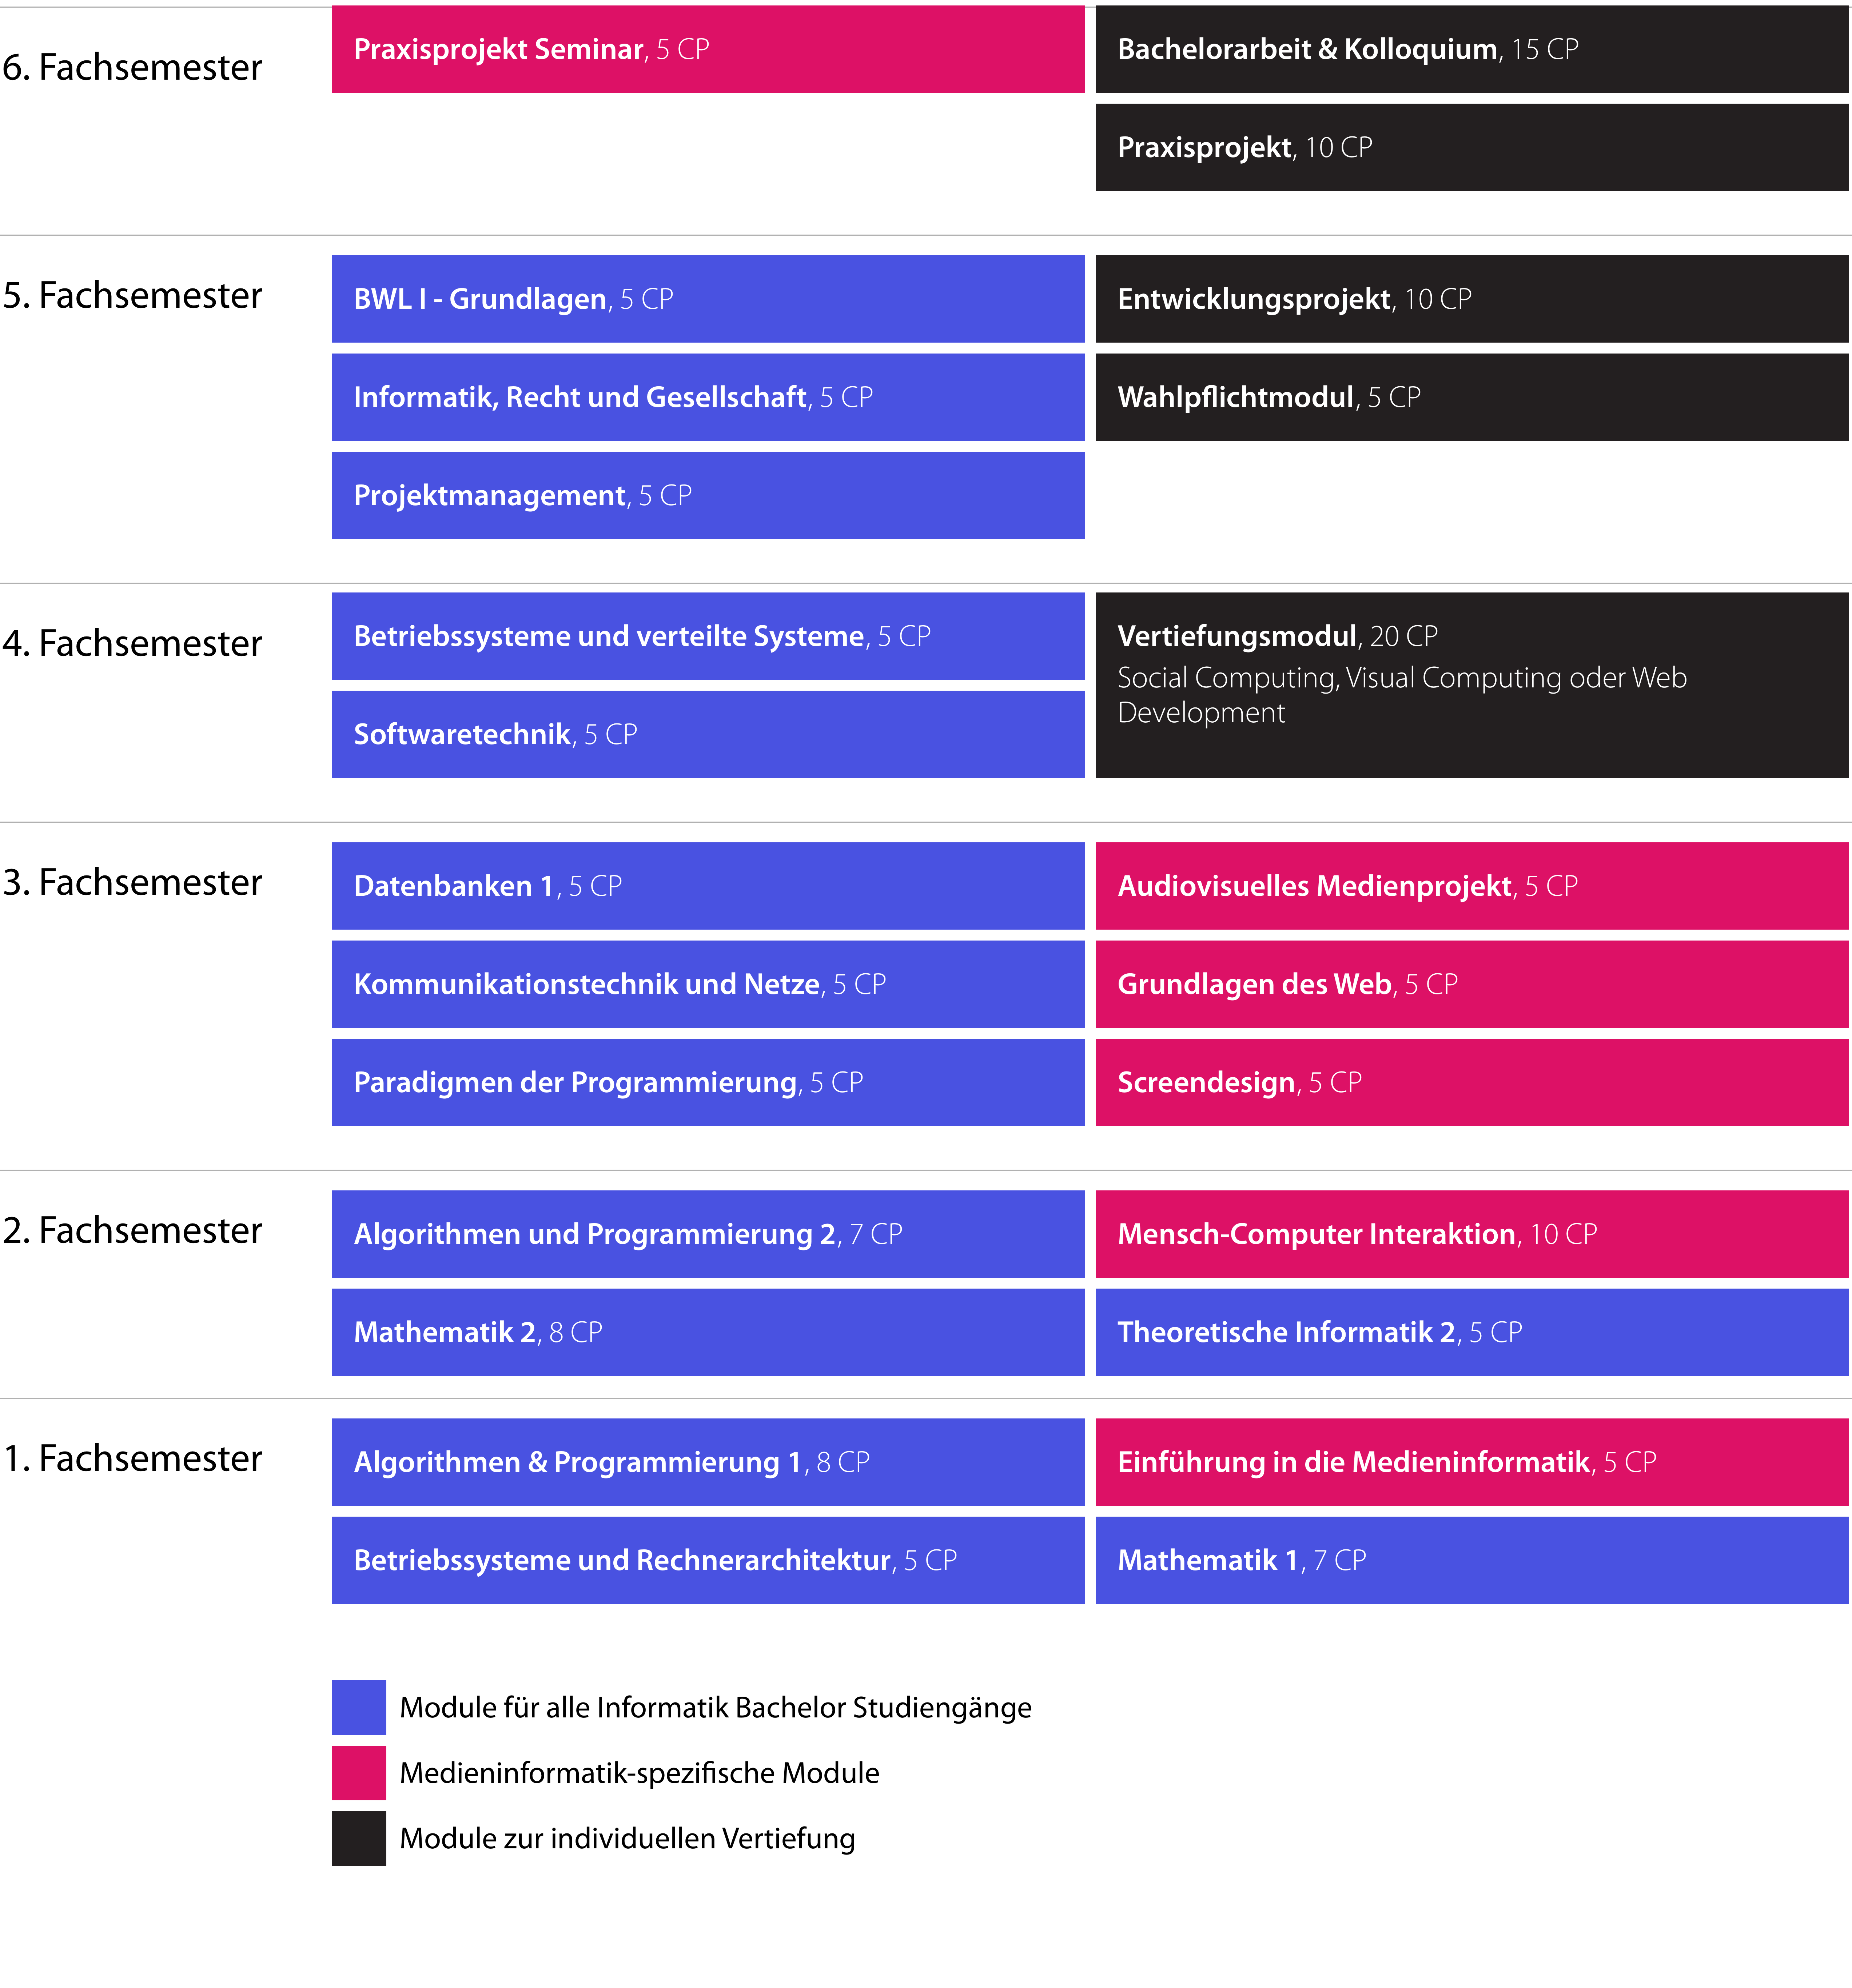
\includegraphics[width=\textwidth]{../anhaenge/bilder/studienverlaufsplan-mi-bachelor.png}
\caption{Studienverlaufsplan Medieninformatik Bachelor}
\end{figure}

\chapter{Algorithmen und Programmierung
1\label{/mi-2017/modulbeschreibungen-bachelor/BA_AlgorithmenundProgrammierung1}}\label{algorithmen-und-programmierung-1pathlabelmi-2017modulbeschreibungen-bachelorbaux5falgorithmenundprogrammierung1}

\begin{modulHead}
\textbf{Modulverantwortlich}: Prof.~Dr.~Frank
Victor
\end{modulHead}
\begin{modulHead}
\textbf{Studiensemester}:
1
\end{modulHead}
\begin{modulHead}
\textbf{Sprache}:
deutsch
\end{modulHead}
\begin{modulHead}
\textbf{Kreditpunkte}:
8
\end{modulHead}
\begin{modulHead}
\textbf{Voraussetzungen nach
Prüfungsordnung}: keine
\end{modulHead}
\begin{modulHead}
\textbf{Typ}:
Pflichtmodul
\end{modulHead}


\section*{Lehrform/SWS\label{/mi-2017/modulbeschreibungen-bachelor/BA_AlgorithmenundProgrammierung1}}\label{lehrformswspathlabelmi-2017modulbeschreibungen-bachelorbaux5falgorithmenundprogrammierung1}

6 SWS: Vorlesung 3 SWS; Übung 1 SWS; Praktikum 2 SWS

\section*{Arbeitsaufwand\label{/mi-2017/modulbeschreibungen-bachelor/BA_AlgorithmenundProgrammierung1}}\label{arbeitsaufwandpathlabelmi-2017modulbeschreibungen-bachelorbaux5falgorithmenundprogrammierung1}

Gesamtaufwand 240h, davon

\begin{itemize}
\tightlist
\item
  54h Vorlesung
\item
  36h Praktikum
\item
  18h Übung
\item
  132h Selbststudium
\end{itemize}

\section*{Angestrebte
Lernergebnisse\label{/mi-2017/modulbeschreibungen-bachelor/BA_AlgorithmenundProgrammierung1}}\label{angestrebte-lernergebnissepathlabelmi-2017modulbeschreibungen-bachelorbaux5falgorithmenundprogrammierung1}

Die Studierenden sollen

\begin{itemize}
\tightlist
\item
  formale und algorithmische Kompetenzen im Bereich der
  Software-Entwicklung erlangen. Hierzu gehören insbesondere die
  Prinzipien der Objektorientierung und die der prozeduralen
  Programmierung.
\item
  die Kompetenz erlangen, strukturierte und unstrukturierte
  Problemstellungen zu analysieren, Lösungen modellbasiert zu entwickeln
  sowie prozedural und objektorientiert umzusetzen.
\item
  Systementwürfe evaluieren und bewerten können, insbesondere sollen sie
  die Arbeitsweise, die Randbedingungen und den Komplexitätsgrad von
  einfachen Algorithmen verstehen.
\item
  die Fähigkeit erlernen, algorithmische Entwurfsmuster zu erkennen und
  anzuwenden
\end{itemize}

\section*{Inhalt\label{/mi-2017/modulbeschreibungen-bachelor/BA_AlgorithmenundProgrammierung1}}\label{inhaltpathlabelmi-2017modulbeschreibungen-bachelorbaux5falgorithmenundprogrammierung1}

\begin{itemize}
\tightlist
\item
  Prozedurale Programmierung am Beispiel von C.
\item
  Objektorientierte Programmierung am Beispiel von Java.
\item
  Kontroll- und Datenstrukturen.
\item
  Modularisierungskonzepte.
\item
  Typkonzepte.
\item
  Grundmuster der objektorientierten Programmierung.
\item
  Elementare Algorithmen und Aufwandsschätzung.
\item
  Entwicklungsumgebungen.
\end{itemize}

\section*{Studien-/Prüfungsleistungen\label{/mi-2017/modulbeschreibungen-bachelor/BA_AlgorithmenundProgrammierung1}}\label{studien-pruxfcfungsleistungenpathlabelmi-2017modulbeschreibungen-bachelorbaux5falgorithmenundprogrammierung1}

Schriftliche Prüfung, sowie erfolgreiche Teilnahme am Praktikum als
Prüfungsvorleistung.

\section*{Medienformen\label{/mi-2017/modulbeschreibungen-bachelor/BA_AlgorithmenundProgrammierung1}}\label{medienformenpathlabelmi-2017modulbeschreibungen-bachelorbaux5falgorithmenundprogrammierung1}

\begin{itemize}
\tightlist
\item
  Beamer-gestützte Vorlesungen (Folien in elektronischer Form)
\item
  Praktikum an Rechnern des Labors
\end{itemize}

\section*{Literatur\label{/mi-2017/modulbeschreibungen-bachelor/BA_AlgorithmenundProgrammierung1}}\label{literaturpathlabelmi-2017modulbeschreibungen-bachelorbaux5falgorithmenundprogrammierung1}

\begin{itemize}
\tightlist
\item
  Vorlesungsunterlagen: Foliensammlung, ausformuliertes Skript,
  Beispiellösungen, Übungsklausuren mit Lösungen
\item
  Fachliteratur: Diverse C-Bücher, u.a.: Kernighan, B.W., Ritchie, D.M.:
  „Programmieren in C``
\item
  Diverse Java-Bücher, u.a.: Bishop, J.: „Java Lernen``
\item
  Sedgewick, R.: „Algorithmen in Java``
\end{itemize}

\chapter{Algorithmen und Programmierung
2\label{/mi-2017/modulbeschreibungen-bachelor/BA_AlgorithmenundProgrammierung2}}\label{algorithmen-und-programmierung-2pathlabelmi-2017modulbeschreibungen-bachelorbaux5falgorithmenundprogrammierung2}

\begin{modulHead}
\textbf{Modulverantwortlich}: Prof.~Dr.~Christian
Kohls
\end{modulHead}
\begin{modulHead}
\textbf{Studiensemester}:
2
\end{modulHead}
\begin{modulHead}
\textbf{Sprache}:
deutsch
\end{modulHead}
\begin{modulHead}
\textbf{Kreditpunkte}:
7
\end{modulHead}
\begin{modulHead}
\textbf{Voraussetzungen nach
Prüfungsordnung}:
keine
\end{modulHead}
\begin{modulHead}
\textbf{Empfohlene
Voraussetzungen}: Algorithmen und Programmierung
1
\end{modulHead}
\begin{modulHead}
\textbf{Typ}:
Pflichtmodul
\end{modulHead}


\section*{Lehrform/SWS\label{/mi-2017/modulbeschreibungen-bachelor/BA_AlgorithmenundProgrammierung2}}\label{lehrformswspathlabelmi-2017modulbeschreibungen-bachelorbaux5falgorithmenundprogrammierung2}

6 SWS: Vorlesung 3 SWS; Übung 1 SWS; Praktikum 2 SWS

\section*{Arbeitsaufwand\label{/mi-2017/modulbeschreibungen-bachelor/BA_AlgorithmenundProgrammierung2}}\label{arbeitsaufwandpathlabelmi-2017modulbeschreibungen-bachelorbaux5falgorithmenundprogrammierung2}

Gesamtaufwand 210h, davon

\begin{itemize}
\tightlist
\item
  54h Vorlesung
\item
  36h Praktikum
\item
  18h Übung
\item
  102h Selbststudium
\end{itemize}

\section*{Angestrebte
Lernergebnisse\label{/mi-2017/modulbeschreibungen-bachelor/BA_AlgorithmenundProgrammierung2}}\label{angestrebte-lernergebnissepathlabelmi-2017modulbeschreibungen-bachelorbaux5falgorithmenundprogrammierung2}

Die Studierende sollen Objektorientierung, die Prinzipien der
Algorithmenentwicklung und grundlegende Algorithmen verstehen und die
Grundstrukturen der Java-Bibliothek anwenden können.

\section*{Inhalt\label{/mi-2017/modulbeschreibungen-bachelor/BA_AlgorithmenundProgrammierung2}}\label{inhaltpathlabelmi-2017modulbeschreibungen-bachelorbaux5falgorithmenundprogrammierung2}

\begin{itemize}
\tightlist
\item
  Basisalgorithmen: Suchen u. Sortieren
\item
  Datenstrukturen
\item
  Dictionaries
\item
  Methodik des objektorientierten Programmierens
\end{itemize}

\section*{Studien-/Prüfungsleistungen\label{/mi-2017/modulbeschreibungen-bachelor/BA_AlgorithmenundProgrammierung2}}\label{studien-pruxfcfungsleistungenpathlabelmi-2017modulbeschreibungen-bachelorbaux5falgorithmenundprogrammierung2}

Schriftliche Prüfung, sowie erfolgreiche Teilnahme am Praktikum als
Prüfungsvorleistung.

\section*{Medienformen\label{/mi-2017/modulbeschreibungen-bachelor/BA_AlgorithmenundProgrammierung2}}\label{medienformenpathlabelmi-2017modulbeschreibungen-bachelorbaux5falgorithmenundprogrammierung2}

\begin{itemize}
\tightlist
\item
  Beamer-gestützte Vorlesungen (Folien in elektronischer Form)
\item
  Praktikum an Rechnern des Labors
\end{itemize}

\section*{Literatur\label{/mi-2017/modulbeschreibungen-bachelor/BA_AlgorithmenundProgrammierung2}}\label{literaturpathlabelmi-2017modulbeschreibungen-bachelorbaux5falgorithmenundprogrammierung2}

\begin{itemize}
\tightlist
\item
  Vorlesungsunterlagen: Foliensammlung, ausformuliertes Skript,
  Beispiellösungen
\item
  Fachliteratur: Bishop, J.: „Java Lernen``
\item
  Sedgewick, R.: „Algorithmen in Java``
\item
  Barnes, J., Kölling, M.: „Java Lernen mit BlueJ``, Verweise auf
  Onlinedokumente
\end{itemize}

\chapter{Audiovisuelles
Medienprojekt\label{/mi-2017/modulbeschreibungen-bachelor/BA_AVM}}\label{audiovisuelles-medienprojektpathlabelmi-2017modulbeschreibungen-bachelorbaux5favm}

\begin{modulHead}
\textbf{Modulverantwortlich}: Prof.~Hans
Kornacher
\end{modulHead}
\begin{modulHead}
\textbf{Studiensemester}:
3
\end{modulHead}
\begin{modulHead}
\textbf{Sprache}:
deutsch
\end{modulHead}
\begin{modulHead}
\textbf{Kreditpunkte}:
5
\end{modulHead}
\begin{modulHead}
\textbf{Voraussetzungen nach
Prüfungsordnung}:
keine
\end{modulHead}
\begin{modulHead}
\textbf{Empfohlene
Voraussetzungen}: Einführung in die
Medieninformatik
\end{modulHead}
\begin{modulHead}
\textbf{Typ}:
Pflichtmodul
\end{modulHead}


\section*{Kurzbeschreibung\label{/mi-2017/modulbeschreibungen-bachelor/BA_AVM}}\label{kurzbeschreibungpathlabelmi-2017modulbeschreibungen-bachelorbaux5favm}

Im Mittelpunkt dieses Moduls steht die digitale audiovisuelle
Medienproduktion in den Formaten Porträt- und Dokumentarfilm.

\section*{Lehrform/SWS\label{/mi-2017/modulbeschreibungen-bachelor/BA_AVM}}\label{lehrformswspathlabelmi-2017modulbeschreibungen-bachelorbaux5favm}

4 SWS: Vorlesung 2 SWS; Projekt 2 SWS

\section*{Arbeitsaufwand\label{/mi-2017/modulbeschreibungen-bachelor/BA_AVM}}\label{arbeitsaufwandpathlabelmi-2017modulbeschreibungen-bachelorbaux5favm}

Gesamtaufwand 150h, davon

\begin{itemize}
\tightlist
\item
  36h Vorlesung
\item
  36h Projektarbeit
\item
  78h Selbststudium
\end{itemize}

\section*{Angestrebte
Lernergebnisse\label{/mi-2017/modulbeschreibungen-bachelor/BA_AVM}}\label{angestrebte-lernergebnissepathlabelmi-2017modulbeschreibungen-bachelorbaux5favm}

\begin{itemize}
\tightlist
\item
  Die Studierenden kennen die grundlegenden Erzählformen und Formate
  audiovisueller Medien und können auf der Basis klassischer
  Erzählmuster eigene audiovisuelle Erzählformen entwickeln.
\item
  Die Studierenden können die in der audiovisuellen Produktion
  auftretende Problemstellungen selbstständig lösen und die verwendeten
  Medientechnologien, wie Videokamera, Tonaufnahmegeräte und
  Schnittsysteme technisch richtig und gestalterisch aussagekräftig
  einzusetzen.
\item
  Sie sind befähigt zur Analyse, Diskussion und zur kritischen
  Betrachtung audiovisueller Medieninhalte.
\item
  Die Studierenden können in den unterschiedlichsten Berufsfeldern
  digitaler audiovisueller Medien die Entwicklung und den Einsatz
  audiovisuellen Content beraten, planen, selbst durchführen und
  verantworten.
\end{itemize}

\section*{Inhalt\label{/mi-2017/modulbeschreibungen-bachelor/BA_AVM}}\label{inhaltpathlabelmi-2017modulbeschreibungen-bachelorbaux5favm}

Im Mittelpunkt dieses Moduls steht die digitale audiovisuelle
Medienproduktion.

Die praktische Umsetzung des Vorlesungsstoffes, die Kommunikation und
Zusammenarbeit im Team und die Präsentation von eigenen Ideen und
Projekten sind die Lerninhalte des Moduls „Audiovisuelles
Medienprojekt``. Neben der Fachkompetenz und Methodenkompetenz stehen in
diesem Modul gerade die sogenannten Softskills Teamfähigkeit und
Kommunikationsfähigkeit im Focus.

Die Projektarbeit gliedert sich dabei in die selbstständige Entwicklung,
Ausarbeitung und Präsentation eines Filmthemas, in die praktische
Umsetzung in einem Filmprojekt und in die Nachbearbeitung und Montage in
einer dramaturgischen Erzählform.

Begleitend zu der Produktion werden folgende fachspezifischen Inhalte
thematisiert und in Übungsaufgaben vertieft:

\begin{itemize}
\tightlist
\item
  Video- und Audioaufnahmetechnik
\item
  Filmsprache
\item
  Lichtsetzung
\item
  Tonaufnahme
\item
  Dokumentarfilm und Interview
\item
  Dramaturgie
\item
  Schnitt und Montage
\end{itemize}

\section*{Studien-/Prüfungsleistungen\label{/mi-2017/modulbeschreibungen-bachelor/BA_AVM}}\label{studien-pruxfcfungsleistungenpathlabelmi-2017modulbeschreibungen-bachelorbaux5favm}

Projektarbeit

\section*{Medienformen\label{/mi-2017/modulbeschreibungen-bachelor/BA_AVM}}\label{medienformenpathlabelmi-2017modulbeschreibungen-bachelorbaux5favm}

\begin{itemize}
\tightlist
\item
  Beamer-gestützte Vorlesungen
\item
  Beispiele aus verschiedenen Medien in elektronischer Form:
  Filmbeispiele, Webvideos
\item
  Audiovisuelle Aufnahme- und Wiedergabegeräte
\end{itemize}

\section*{Literatur\label{/mi-2017/modulbeschreibungen-bachelor/BA_AVM}}\label{literaturpathlabelmi-2017modulbeschreibungen-bachelorbaux5favm}

\begin{itemize}
\tightlist
\item
  James Monaco, Film verstehen, Rowolth Taschenbuch Verlag Hamburg,
  1980, ISBN 3-499-162717
\item
  Syd Field, Drehbuchschreiben für Film und Fernsehen, München 2003,
  ISBN 354836473X
\item
  Steven D. Katz, Die Richtige Einstellung, Zweitausendeins, Frankfurt
  a.M.1998,ISBN 3-86150-229-1
\item
  David Lewis Yewdall, Practical Art of Motion Picture Sound, Focal
  Press, USA 2003, ISBN 0-240-80525-9
\item
  Hans Kornacher \& Manfred Stross, Dokumentarisches Videofilmen,
  Augustus Verlag, Augsburg, 1992, ISBN 3-8043-5474-2
\item
  Hans Beller Hg., Handbuch der Filmmontage, München: TR-Verlagsunion,
  1993, ISBN 3-8058-2357-6
\item
  Karel Reisz, Gavin Millar, Geschichte und Technik der Filmmontage,
  München: Filmlandpresse, 1988, ISBN 3-88690-071-1
\item
  Chris Vogler, Die Reise des Drehbuchschreibens, Verlag Zweitausendeins
\end{itemize}

\chapter{Bachelorarbeit\label{/mi-2017/modulbeschreibungen-bachelor/BA_Bachelorarbeit}}\label{bachelorarbeitpathlabelmi-2017modulbeschreibungen-bachelorbaux5fbachelorarbeit}

\begin{modulHead}
\textbf{Modulverantwortlich}: alle Informatik
Professoren
\end{modulHead}
\begin{modulHead}
\textbf{Studiensemester}:
6
\end{modulHead}
\begin{modulHead}
\textbf{Sprache}:
deutsch
\end{modulHead}
\begin{modulHead}
\textbf{Kreditpunkte}:
12
\end{modulHead}
\begin{modulHead}
\textbf{Voraussetzungen nach
Prüfungsordnung}: alle Modulprüfungen außer Bachelorarbeit und
Kolloquium bestanden
\end{modulHead}
\begin{modulHead}
\textbf{Typ}:
Pflichtmodul
\end{modulHead}


\section*{Lehrform/SWS\label{/mi-2017/modulbeschreibungen-bachelor/BA_Bachelorarbeit}}\label{lehrformswspathlabelmi-2017modulbeschreibungen-bachelorbaux5fbachelorarbeit}

Angeleitetes, eigenverantwortliches Arbeiten

\section*{Arbeitsaufwand\label{/mi-2017/modulbeschreibungen-bachelor/BA_Bachelorarbeit}}\label{arbeitsaufwandpathlabelmi-2017modulbeschreibungen-bachelorbaux5fbachelorarbeit}

360 Stunden

\section*{Angestrebte
Lernergebnisse\label{/mi-2017/modulbeschreibungen-bachelor/BA_Bachelorarbeit}}\label{angestrebte-lernergebnissepathlabelmi-2017modulbeschreibungen-bachelorbaux5fbachelorarbeit}

Die Bachelorarbeit soll zeigen, dass der Prüfling befähigt ist,
innerhalb einer vorgegebenen Frist eine praxisorientierte Aufgabe aus
seinem Fachgebiet sowohl in ihren fachlichen Einzelheiten als auch in
den fachübergreifenden Zusammenhängen nach wissenschaftlichen,
fachpraktischen und gestalterischen Methoden selbständig zu bearbeiten.
Die Bachelorarbeit ist in der Regel eine eigenständige Untersuchung mit
einer Aufgabenstellung aus der Medieninformatik und einer ausführlichen
Beschreibung und Erläuterung ihrer Lösung. In fachlich geeigneten Fällen
kann sie auch eine schriftliche Hausarbeit mit fachliterarischem Inhalt
sein.

\section*{Inhalt\label{/mi-2017/modulbeschreibungen-bachelor/BA_Bachelorarbeit}}\label{inhaltpathlabelmi-2017modulbeschreibungen-bachelorbaux5fbachelorarbeit}

Selbstständiges wissenschaftliches, fachpraktisches und gestalterisches
Bearbeiten einer Aufgabenstellung.

\section*{Studien-/Prüfungsleistungen\label{/mi-2017/modulbeschreibungen-bachelor/BA_Bachelorarbeit}}\label{studien-pruxfcfungsleistungenpathlabelmi-2017modulbeschreibungen-bachelorbaux5fbachelorarbeit}

Schriftliche Ausarbeitung, ggf. Projektarbeit mit entsprechenden
Artefakten.

\chapter{Bachelor
Kolloquium\label{/mi-2017/modulbeschreibungen-bachelor/BA_Bachelorkolloquium}}\label{bachelor-kolloquiumpathlabelmi-2017modulbeschreibungen-bachelorbaux5fbachelorkolloquium}

\begin{modulHead}
\textbf{Modulverantwortlich}: alle Informatik
Professoren
\end{modulHead}
\begin{modulHead}
\textbf{Studiensemester}:
6
\end{modulHead}
\begin{modulHead}
\textbf{Sprache}:
deutsch
\end{modulHead}
\begin{modulHead}
\textbf{Kreditpunkte}:
3
\end{modulHead}
\begin{modulHead}
\textbf{Voraussetzungen nach
Prüfungsordnung}: alle Modulprüfungen außer Bachelor Kolloquium
bestanden
\end{modulHead}
\begin{modulHead}
\textbf{Typ}:
Pflichtmodul
\end{modulHead}


\section*{Lehrform/SWS\label{/mi-2017/modulbeschreibungen-bachelor/BA_Bachelorkolloquium}}\label{lehrformswspathlabelmi-2017modulbeschreibungen-bachelorbaux5fbachelorkolloquium}

Angeleitetes, eigenverantwortliches Arbeiten

\section*{Arbeitsaufwand\label{/mi-2017/modulbeschreibungen-bachelor/BA_Bachelorkolloquium}}\label{arbeitsaufwandpathlabelmi-2017modulbeschreibungen-bachelorbaux5fbachelorkolloquium}

90 Stunden

\section*{Angestrebte
Lernergebnisse\label{/mi-2017/modulbeschreibungen-bachelor/BA_Bachelorkolloquium}}\label{angestrebte-lernergebnissepathlabelmi-2017modulbeschreibungen-bachelorbaux5fbachelorkolloquium}

Das Kolloquium dient der Feststellung, ob der Prüfling befähigt ist, die
Ergebnisse der Bachelorarbeit, ihre fachlichen Grundlagen, ihre
fachübergreifenden Zusammenhänge und ihre außerfachlichen Bezüge
mündlich darzustellen und selbständig zu begründen und ihre Bedeutung
für die Praxis einzuschätzen. Dabei soll auch die Bearbeitung des Themas
der Bachelorarbeit mit dem Prüfling erörtert werden.

\section*{Inhalt\label{/mi-2017/modulbeschreibungen-bachelor/BA_Bachelorkolloquium}}\label{inhaltpathlabelmi-2017modulbeschreibungen-bachelorbaux5fbachelorkolloquium}

Vortrag über das Thema der Bachelorarbeit, Fachdiskussion und mündliche
Verteidigung der Arbeit im Kontext der Medieninformatik.

\section*{Studien-/Prüfungsleistungen\label{/mi-2017/modulbeschreibungen-bachelor/BA_Bachelorkolloquium}}\label{studien-pruxfcfungsleistungenpathlabelmi-2017modulbeschreibungen-bachelorbaux5fbachelorkolloquium}

mündliche Prüfung, Vortrag

\chapter{Betriebssysteme und verteilte
Systeme\label{/mi-2017/modulbeschreibungen-bachelor/BA_betriebssysteme-und-verteile-systeme}}\label{betriebssysteme-und-verteilte-systemepathlabelmi-2017modulbeschreibungen-bachelorbaux5fbetriebssysteme-und-verteile-systeme}

\begin{modulHead}
\textbf{Modulverantwortlich}: Prof.~Dr.~Matthias
Böhmer, Prof.~Dr.~Lutz
Köhler
\end{modulHead}
\begin{modulHead}
\textbf{Studiensemester}:
4
\end{modulHead}
\begin{modulHead}
\textbf{Sprache}:
deutsch
\end{modulHead}
\begin{modulHead}
\textbf{Kreditpunkte}:
5
\end{modulHead}
\begin{modulHead}
\textbf{Voraussetzungen nach
Prüfungsordnung}:
keine
\end{modulHead}
\begin{modulHead}
\textbf{Empfohlene
Voraussetzungen}: Einführung in die Medieninformatik, Algorithmen und
Programmierung
\end{modulHead}
\begin{modulHead}
\textbf{Typ}:
Pflichtmodul
\end{modulHead}


\section*{Kurzbeschreibung\label{/mi-2017/modulbeschreibungen-bachelor/BA_betriebssysteme-und-verteile-systeme}}\label{kurzbeschreibungpathlabelmi-2017modulbeschreibungen-bachelorbaux5fbetriebssysteme-und-verteile-systeme}

Systemprogrammierung am Beispiel von UNIX.

\section*{Lehrform/SWS\label{/mi-2017/modulbeschreibungen-bachelor/BA_betriebssysteme-und-verteile-systeme}}\label{lehrformswspathlabelmi-2017modulbeschreibungen-bachelorbaux5fbetriebssysteme-und-verteile-systeme}

4 SWS: Vorlesung 2 SWS; Praktikum 2 SWS

\section*{Arbeitsaufwand\label{/mi-2017/modulbeschreibungen-bachelor/BA_betriebssysteme-und-verteile-systeme}}\label{arbeitsaufwandpathlabelmi-2017modulbeschreibungen-bachelorbaux5fbetriebssysteme-und-verteile-systeme}

Gesamtaufwand 150h, davon

\begin{itemize}
\tightlist
\item
  36h Vorlesung
\item
  36h Praktikum
\item
  78h Selbststudium
\end{itemize}

\section*{Angestrebte
Lernergebnisse\label{/mi-2017/modulbeschreibungen-bachelor/BA_betriebssysteme-und-verteile-systeme}}\label{angestrebte-lernergebnissepathlabelmi-2017modulbeschreibungen-bachelorbaux5fbetriebssysteme-und-verteile-systeme}

Die Studierenden können den Aufbau von Betriebssystemen am Beispiel UNIX
erläutern, indem sie

\begin{itemize}
\tightlist
\item
  die Ziele der Entwicklung von UNIX nennen und beschreiben,
\item
  die Hauptaufgaben von Betriebssystemen nennen und beschreiben,
\item
  den Aufbau von Betriebssystemen darstellen und erklären,
\end{itemize}

um die verschiedenen Bestandteile und Konzepte von Betriebssystemen
nutzen zu können.

Die Studierenden können eigene C-Programme für verteilte Systeme
erstellen, indem sie

\begin{itemize}
\tightlist
\item
  einen Computer über die Shell bedienen und dort eigene Programme
  ausführbar machen,
\item
  Daten mittels Systemschnittstellen in Dateien speichern, daraus lesen
  und diese verwalten,
\item
  Sockets für Client- und Serverprogramme nutzen und Daten darüber
  senden und empfangen,
\item
  Prozesse für nebenläufige Programmabläufe erzeugen,
\item
  Kommunikation zwischen Prozessen mit Shared Memory, Pipes und Message
  Queues realisieren,
\item
  Race Conditions erkennen, kritische Abschnitte festlegen und Prozesse
  synchronisieren,
\item
  die Lösungen klassischer Synchronisationsprobleme kennen und nutzen,
\end{itemize}

um später hardware- oder systemnahe Software für verteilte Systeme zu
entwickeln oder zu bewerten, bspw. im Bereich »Internet of Things«

Die Studierenden können theoretische Grundlagen von Betriebssystemen
erörtern, indem sie

\begin{itemize}
\tightlist
\item
  Programme und Prozesse unterscheiden und letztere mit ihren Zuständen
  modellieren,
\item
  verschiedene Strategien für das Scheduling von Prozessen anwenden und
  bewerten,
\item
  die Organisation des Speichers auf einem Datenträger erklären und
  darstellen,
\item
  die Abbildung von Prozessen im Arbeitsspeicher erklären und
  verschiedene Ansätze zur Verwaltung erläutern,
\end{itemize}

um später Auswirkungen von Betriebssystemvorgängen auf eigene Programme
zu erkennen und darauf zu reagieren.

\section*{Inhalt\label{/mi-2017/modulbeschreibungen-bachelor/BA_betriebssysteme-und-verteile-systeme}}\label{inhaltpathlabelmi-2017modulbeschreibungen-bachelorbaux5fbetriebssysteme-und-verteile-systeme}

Systemprogrammierung am Beispiel von UNIX:

\begin{itemize}
\tightlist
\item
  Shell-Programmierung
\item
  Prozess-Modelle
\item
  Prozess-Erzeugung und Synchronisation
\item
  UNIX-Prozesse und elementare Synchronisation
\item
  Pipes
\item
  Shared Memory
\item
  Synchronisationsprimitive für den wechselseitigen Ausschluss
\item
  Semaphoren
\item
  Nachrichtenwarteschlangen
\item
  Dateisysteme
\item
  TCP/IP
\item
  Sockets
\item
  Remote Procedure Call
\item
  Strategien zum Scheduling und zur Speicherverwaltung
\item
  Klassische Synchronisationsprobleme
\end{itemize}

\section*{Studien-/Prüfungsleistungen\label{/mi-2017/modulbeschreibungen-bachelor/BA_betriebssysteme-und-verteile-systeme}}\label{studien-pruxfcfungsleistungenpathlabelmi-2017modulbeschreibungen-bachelorbaux5fbetriebssysteme-und-verteile-systeme}

Schriftliche Prüfung, sowie erfolgreiche Teilnahme am Praktikum als
Prüfungsvorleistung.

\section*{Medienformen\label{/mi-2017/modulbeschreibungen-bachelor/BA_betriebssysteme-und-verteile-systeme}}\label{medienformenpathlabelmi-2017modulbeschreibungen-bachelorbaux5fbetriebssysteme-und-verteile-systeme}

Foliensammlung, ausformuliertes Skript, Beispiellösungen

\section*{Literatur\label{/mi-2017/modulbeschreibungen-bachelor/BA_betriebssysteme-und-verteile-systeme}}\label{literaturpathlabelmi-2017modulbeschreibungen-bachelorbaux5fbetriebssysteme-und-verteile-systeme}

\begin{itemize}
\tightlist
\item
  Tanenbaum, A. S.: „Moderne Betriebssysteme``
\item
  Brown, C.: „Programmieren verteilter UNIX-Anwendungen``
\item
  Kernighan, B. W., Pike, R.: „Der UNIX-Werkzeugkasten``
\item
  Ehses, E., Köhler, L., Stenzel, H., Victor, F. „Betriebssysteme: Ein
  Lehrbuch mit Übungen zur Systemprogrammierung in UNIX/Linux``
\end{itemize}

\chapter{BWL I -
Grundlagen\label{/mi-2017/modulbeschreibungen-bachelor/BA_BWL1}}\label{bwl-i---grundlagenpathlabelmi-2017modulbeschreibungen-bachelorbaux5fbwl1}

\begin{modulHead}
\textbf{Modulverantwortlich}: Prof.~Dr.~Monika
Engelen
\end{modulHead}
\begin{modulHead}
\textbf{Studiensemester}:
5
\end{modulHead}
\begin{modulHead}
\textbf{Sprache}:
deutsch
\end{modulHead}
\begin{modulHead}
\textbf{Kreditpunkte}:
5
\end{modulHead}
\begin{modulHead}
\textbf{Voraussetzungen nach
Prüfungsordnung}: keine
\end{modulHead}
\begin{modulHead}
\textbf{Typ}:
Pflichtmodul
\end{modulHead}


\section*{Lehrform/SWS\label{/mi-2017/modulbeschreibungen-bachelor/BA_BWL1}}\label{lehrformswspathlabelmi-2017modulbeschreibungen-bachelorbaux5fbwl1}

4 SWS: Vorlesung 2 SWS; Übung 2 SWS

\section*{Arbeitsaufwand\label{/mi-2017/modulbeschreibungen-bachelor/BA_BWL1}}\label{arbeitsaufwandpathlabelmi-2017modulbeschreibungen-bachelorbaux5fbwl1}

Gesamtaufwand 150h, davon

\begin{itemize}
\tightlist
\item
  30h Vorlesung
\item
  30h Übung
\item
  90h Selbststudium
\end{itemize}

\section*{Angestrebte
Lernergebnisse\label{/mi-2017/modulbeschreibungen-bachelor/BA_BWL1}}\label{angestrebte-lernergebnissepathlabelmi-2017modulbeschreibungen-bachelorbaux5fbwl1}

Die Studierenden verstehen die wichtigsten Entscheidungsbereiche
wirtschaftlichen Handeln und können diese anwenden. Sie können
grundlegenden Entscheidungen im Rahmen einer Unternehmensgründung, die
Aufgaben der Unternehmensführung wie die Konzeption einer tragfähigen
Strategie, und die Aufgaben der Teilbereiche Produktion, Absatz und
Marketing sowie Investition und Finanzierung beschreiben und beurteilen.
Investitionsentscheidungen können die Studierenden informationsgestützt
treffen indem sie die Kalkulationsverfahren der Investitionsrechnung
anwenden und auswerten. Die Veranstaltung bereitet die Studierenden für
weitere BWL-Veranstaltungen ihres Studiums, sowie darauf, in ihrem
Berufsleben wirtschaftliche Konzepte im Unternehmenskontext anzuwenden,
vor.

\section*{Inhalt\label{/mi-2017/modulbeschreibungen-bachelor/BA_BWL1}}\label{inhaltpathlabelmi-2017modulbeschreibungen-bachelorbaux5fbwl1}

\begin{itemize}
\tightlist
\item
  Grundlagen
\item
  Unternehmensführung 1: Ziele, Planung und Entscheidung
\item
  Investition und Finanzierung
\item
  Unternehmensführung 2: Ausführung und Kontrolle
\item
  Konstitutive Entscheidungen
\item
  Produktion
\item
  Absatz und Marketing
\end{itemize}

\section*{Studien-/Prüfungsleistungen\label{/mi-2017/modulbeschreibungen-bachelor/BA_BWL1}}\label{studien-pruxfcfungsleistungenpathlabelmi-2017modulbeschreibungen-bachelorbaux5fbwl1}

schriftliche Prüfung

\section*{Literatur\label{/mi-2017/modulbeschreibungen-bachelor/BA_BWL1}}\label{literaturpathlabelmi-2017modulbeschreibungen-bachelorbaux5fbwl1}

\begin{itemize}
\tightlist
\item
  Wöhe (2016): Einführung in die Allgemeine Betriebswirtschaftslehre,
  26. Aufl.
\end{itemize}

\chapter{Datenbanken
1\label{/mi-2017/modulbeschreibungen-bachelor/BA_Datenbanken1}}\label{datenbanken-1pathlabelmi-2017modulbeschreibungen-bachelorbaux5fdatenbanken1}

\begin{modulHead}
\textbf{Modulverantwortlich}: Prof.~Dr.~Birgit
Bertelsmeier, Prof.~Dr.~Heide
Faeskorn-Woyke
\end{modulHead}
\begin{modulHead}
\textbf{Studiensemester}:
3
\end{modulHead}
\begin{modulHead}
\textbf{Sprache}:
deutsch
\end{modulHead}
\begin{modulHead}
\textbf{Kreditpunkte}:
5
\end{modulHead}
\begin{modulHead}
\textbf{Voraussetzungen nach
Prüfungsordnung}: Klausurteilnahme nur bei bestandenem
DBS1-Praktikum
\end{modulHead}
\begin{modulHead}
\textbf{Typ}:
Pflichtmodul
\end{modulHead}


\section*{Lehrform/SWS\label{/mi-2017/modulbeschreibungen-bachelor/BA_Datenbanken1}}\label{lehrformswspathlabelmi-2017modulbeschreibungen-bachelorbaux5fdatenbanken1}

4 SWS: Vorlesung 2 SWS; Übung 1 SWS; Praktikum 1 SWS

\section*{Arbeitsaufwand\label{/mi-2017/modulbeschreibungen-bachelor/BA_Datenbanken1}}\label{arbeitsaufwandpathlabelmi-2017modulbeschreibungen-bachelorbaux5fdatenbanken1}

Gesamtaufwand 150h, davon

\begin{itemize}
\tightlist
\item
  36h Vorlesung
\item
  18h Praktikum
\item
  18h Übung
\item
  78h Selbststudium
\end{itemize}

\section*{Angestrebte
Lernergebnisse\label{/mi-2017/modulbeschreibungen-bachelor/BA_Datenbanken1}}\label{angestrebte-lernergebnissepathlabelmi-2017modulbeschreibungen-bachelorbaux5fdatenbanken1}

Die Studierenden sollen

\begin{itemize}
\tightlist
\item
  über ein einheitliches konsistentes Begriffsgebäude bezüglich der
  Datenbankthematik verfügen,
\item
  die theoretischen Grundlagen von Datenbanksystemen am Beispiel
  relationaler und objektrelationaler Datenbanksysteme verstanden haben,
  insbesondere die relationale Algebra, die Normalisierung sowie
  funktionale Abhängigkeiten
\item
  in der Lage sein, diese Erkenntnisse im Rahmen der Modellierung und
  Implementierung von Datenbankschemata praktisch anzuwenden,
\item
  komplexere Datenbankanfragen, Datendefinitionen und Datenänderungen
  über SQL programmieren~ können
\item
  ein SQL-Statement tunen können
\item
  mit dem Transaktionsbegriff, der Mehrbenutzersynchronisation und
  Verfahren zur Fehlererholung sowie zur Sicherung der Datenintegrität
  vertraut sein
\end{itemize}

\section*{Inhalt\label{/mi-2017/modulbeschreibungen-bachelor/BA_Datenbanken1}}\label{inhaltpathlabelmi-2017modulbeschreibungen-bachelorbaux5fdatenbanken1}

\begin{itemize}
\tightlist
\item
  Grundbegriffe und Architektur von Datenbanken
\item
  Ein Vorgehensmodell zur Erstellung eines Datenbanksystems
\item
  Grundlagen des relationalen Modells
\item
  Relationale Algebra
\item
  Anfrageoptimierung
\item
  Funktionale Abhängigkeiten
\item
  Datenintegrität
\item
  Normalisierung
\item
  Datenmodellierung (Entity Relationship Modell) und Implementierung am
  Beispiel eines relationalen Datenbanksystems
\item
  Datenbanksprache SQL: DDL, DML, DAL, Integritätsbedingungen und
  Constraints unter dem jeweils aktuellen SQL-Standard, zur Zeit SQL2013
\item
  Transaktionskonzepte, Mehrbenutzersynchronisation, Fehlererholung und
  Datensicherheit
\end{itemize}

\section*{Studien-/Prüfungsleistungen\label{/mi-2017/modulbeschreibungen-bachelor/BA_Datenbanken1}}\label{studien-pruxfcfungsleistungenpathlabelmi-2017modulbeschreibungen-bachelorbaux5fdatenbanken1}

Schriftliche Prüfung, sowie erfolgreiche Teilnahme am Praktikum als
Prüfungsvorleistung.

Semesterbegleitende Multiple-Choice-Tests mit Punkten für die Klausur.

\section*{Medienformen\label{/mi-2017/modulbeschreibungen-bachelor/BA_Datenbanken1}}\label{medienformenpathlabelmi-2017modulbeschreibungen-bachelorbaux5fdatenbanken1}

\begin{itemize}
\tightlist
\item
  Folien gestützer Vortrag - aber nur sehr selten
\item
  I.d.R. erarbeiten der Theorie anhand von überschaubaren
  Problemstellungen und deren in der Veranstaltung entwickelten Lösungen
  - hauptsächliches Vorgehen
\item
  Fragen der Studierenden beantworten - sehr erwünscht!
\item
  Ilias zur Bereitstellung aller Informationen (Aktuelles, Links,
  Folien, Praktikums-/Übungsaufgaben, wie auch Lösungen)
\item
  edb, die DB-eLearning-Plattform der TH Köln
\item
  DB-Wiki, das Online Lexikon für Datenbank-Themen
\end{itemize}

\section*{Literatur\label{/mi-2017/modulbeschreibungen-bachelor/BA_Datenbanken1}}\label{literaturpathlabelmi-2017modulbeschreibungen-bachelorbaux5fdatenbanken1}

\begin{itemize}
\tightlist
\item
  Elmasri, R.; Navathe, S. B.: Grundlagen von Datenbanksystemen.
  Pearson-Studium. 2009
\item
  Faeskorn-Woyke, H.; Bertelsmeier, B.; Riemer, P.; Bauer, E.:
  Datenbanksysteme - Theorie und Praxis mit SQL2003, Oracle und MySQL.
  Pearson-Studium. 2. Aufl. 2011
\item
  Kemper, A.; Eickler, A.: Datenbanksysteme -- Eine Einführung.
  Oldenbourg-Verlag, 2015
\item
  Saake, G., Sattler, K.-U.; Heuer, A.: Datenbanken - Konzepte und
  Sprachen. Mitp/bhv, 2013
\item
  Vossen, G.: Datenmodelle, Datenbanksprachen,
  Datenbankmanagementsysteme. Oldenbourg-Verlag, 2008
\end{itemize}

\chapter{Einführung in Betriebssysteme und
Rechnerarchitektur\label{/mi-2017/modulbeschreibungen-bachelor/BA_EinfhrunginBetriebssystemeundRechnerarchitektur}}\label{einfuxfchrung-in-betriebssysteme-und-rechnerarchitekturpathlabelmi-2017modulbeschreibungen-bachelorbaux5feinfhrunginbetriebssystemeundrechnerarchitektur}

\begin{modulHead}
\textbf{Modulverantwortlich}: Prof.~Dr.~Stefan
Karsch
\end{modulHead}
\begin{modulHead}
\textbf{Studiensemester}:
1
\end{modulHead}
\begin{modulHead}
\textbf{Sprache}:
deutsch
\end{modulHead}
\begin{modulHead}
\textbf{Kreditpunkte}:
5
\end{modulHead}
\begin{modulHead}
\textbf{Voraussetzungen nach
Prüfungsordnung}: keine
\end{modulHead}
\begin{modulHead}
\textbf{Typ}:
Pflichtmodul
\end{modulHead}


\section*{Lehrform/SWS\label{/mi-2017/modulbeschreibungen-bachelor/BA_EinfhrunginBetriebssystemeundRechnerarchitektur}}\label{lehrformswspathlabelmi-2017modulbeschreibungen-bachelorbaux5feinfhrunginbetriebssystemeundrechnerarchitektur}

4 SWS: Vorlesung 2 SWS; Übung 2 SWS

\section*{Arbeitsaufwand\label{/mi-2017/modulbeschreibungen-bachelor/BA_EinfhrunginBetriebssystemeundRechnerarchitektur}}\label{arbeitsaufwandpathlabelmi-2017modulbeschreibungen-bachelorbaux5feinfhrunginbetriebssystemeundrechnerarchitektur}

Gesamtaufwand 150h, davon

\begin{itemize}
\tightlist
\item
  36h Vorlesung
\item
  36h Übung
\item
  78h Selbststudium
\end{itemize}

\section*{Angestrebte
Lernergebnisse\label{/mi-2017/modulbeschreibungen-bachelor/BA_EinfhrunginBetriebssystemeundRechnerarchitektur}}\label{angestrebte-lernergebnissepathlabelmi-2017modulbeschreibungen-bachelorbaux5feinfhrunginbetriebssystemeundrechnerarchitektur}

Die Studierenden sollen die Basiskonzepte und Grundlagen der
Betriebssysteme und der Rechnerarchitektur kennen und verstehen, sowie
ein einheitliches konsistentes Begriffsgebäude zu, teilweise aus der
persönlichen Praxis bekannten, Sachverhalten der IT aufbauen und
anwenden können.

\section*{Inhalt\label{/mi-2017/modulbeschreibungen-bachelor/BA_EinfhrunginBetriebssystemeundRechnerarchitektur}}\label{inhaltpathlabelmi-2017modulbeschreibungen-bachelorbaux5feinfhrunginbetriebssystemeundrechnerarchitektur}

\begin{itemize}
\tightlist
\item
  Betriebssysteme aus Nutzersicht: Dateisysteme, Parallele Prozesse,
  Sicherheit in Betriebssystemen
\item
  bei Rechnerkomponenten: grundlegende Architekturen, Darstellung von
  Daten, interne Bussysteme, Prozessoren, Festplatten,
  Peripherieschnittstellen, Parallelrechner
\end{itemize}

\section*{Studien-/Prüfungsleistungen\label{/mi-2017/modulbeschreibungen-bachelor/BA_EinfhrunginBetriebssystemeundRechnerarchitektur}}\label{studien-pruxfcfungsleistungenpathlabelmi-2017modulbeschreibungen-bachelorbaux5feinfhrunginbetriebssystemeundrechnerarchitektur}

Schriftliche Prüfung.

\section*{Literatur\label{/mi-2017/modulbeschreibungen-bachelor/BA_EinfhrunginBetriebssystemeundRechnerarchitektur}}\label{literaturpathlabelmi-2017modulbeschreibungen-bachelorbaux5feinfhrunginbetriebssystemeundrechnerarchitektur}

\begin{itemize}
\tightlist
\item
  Vorlesungsunterlagen: kommentierte Foliensammlung
\item
  Tanenbaum: „Rechnerarchitektur``
\item
  Tanenbaum: „Modern Operating Systems``
\end{itemize}

\chapter{Einführung in die
Medieninformatik\label{/mi-2017/modulbeschreibungen-bachelor/BA_EinfhrungindieMedieninformatik}}\label{einfuxfchrung-in-die-medieninformatikpathlabelmi-2017modulbeschreibungen-bachelorbaux5feinfhrungindiemedieninformatik}

\begin{modulHead}
\textbf{Modulverantwortlich}: Prof.~Dr.~Martin
Eisemann, Prof.~Dr.~Kristian Fischer, Prof.~Dr.~Gerhard Hartmann,
Prof.~Dr.~Christian Kohls, Prof.~Hans Kornacher, Prof.~Christian Noss,
Prof.~Dr.~Mario
Winter
\end{modulHead}
\begin{modulHead}
\textbf{Studiensemester}:
1
\end{modulHead}
\begin{modulHead}
\textbf{Sprache}:
deutsch
\end{modulHead}
\begin{modulHead}
\textbf{Kreditpunkte}:
5
\end{modulHead}
\begin{modulHead}
\textbf{Voraussetzungen nach
Prüfungsordnung}: keine
\end{modulHead}
\begin{modulHead}
\textbf{Typ}:
Pflichtmodul
\end{modulHead}


\section*{Lehrform/SWS\label{/mi-2017/modulbeschreibungen-bachelor/BA_EinfhrungindieMedieninformatik}}\label{lehrformswspathlabelmi-2017modulbeschreibungen-bachelorbaux5feinfhrungindiemedieninformatik}

4 SWS: Seminar 3 SWS; Übung 1 SWS

Seminar mit eingebetteten Übungselementen und Projektarbeit.

\section*{Arbeitsaufwand\label{/mi-2017/modulbeschreibungen-bachelor/BA_EinfhrungindieMedieninformatik}}\label{arbeitsaufwandpathlabelmi-2017modulbeschreibungen-bachelorbaux5feinfhrungindiemedieninformatik}

Gesamtaufwand 150h, davon

\begin{itemize}
\tightlist
\item
  30h Seminar
\item
  10h Übung
\item
  40h Projekt
\item
  70h Selbststudium
\end{itemize}

\section*{Angestrebte
Lernergebnisse\label{/mi-2017/modulbeschreibungen-bachelor/BA_EinfhrungindieMedieninformatik}}\label{angestrebte-lernergebnissepathlabelmi-2017modulbeschreibungen-bachelorbaux5feinfhrungindiemedieninformatik}

Die Studierenden können die inhaltlichen Ausrichtungen und die
Zielsetzungen der Lehr- und Anwendungsdisziplin Medieninformatik
benennen und gegenüber verwandten oder ähnlichen Disziplinen abgrenzen.

Die Studierenden kennen Grundkonzepte der Informatik (z.B.
Anforderungen) sowie audiovisueller und interaktiver Medientechnologien,
kennen architekturelle Alternativen interaktiver Systeme und kennen
Gestaltungsdimensionen für deren Informations- und Kommunikationsinhalte
und können diese Kenntnisse auf eine gegebene Problemstellung anwenden.

Die Studierenden sind sensibilisiert für Modellierungs- und
Entwicklungsaufgaben von medienbasierten Software-Systemen zur
Unterstützung menschlichen Handelns in betrieblichen und privaten
Kontexten.

Sie kennen grundlegende Konzepte, Prozesse/Verfahren und Modelle der
Medieninformatik und haben erste Projekterfahrungen gesammelt. Sie
können Systemkonzeptionen, zugehörige Modellierungen, Abwägungen und
Artefakte für ein Fachpublikum angemessen dokumentieren und mittels
verschiedener medialer Formen kommunizieren.

\section*{Inhalt\label{/mi-2017/modulbeschreibungen-bachelor/BA_EinfhrungindieMedieninformatik}}\label{inhaltpathlabelmi-2017modulbeschreibungen-bachelorbaux5feinfhrungindiemedieninformatik}

Workshops zu grundlegenden projektrelevanten Themenfeldern (wie:
Datenmodellierung, Pseudo-Code, Kommunikation in verteilen medialen
Systeme, Visual Thinking, Storytelling, Anforderungen) und deren
Anwendung, illustriert anhand von Fallstudien.

Teambasiertes Projekt, welches ausgehend von Kontextszenarien eine (oder
mehrere) Problemstellung(en) umreist, zu dem Lösungen konzipiert und
prototypisch umgesetzt, dokumentiert und einem Fachpublikum präsentiert
werden müssen.

\section*{Studien-/Prüfungsleistungen\label{/mi-2017/modulbeschreibungen-bachelor/BA_EinfhrungindieMedieninformatik}}\label{studien-pruxfcfungsleistungenpathlabelmi-2017modulbeschreibungen-bachelorbaux5feinfhrungindiemedieninformatik}

Projektpräsentation(30\%) und schriftliche Ausarbeitung(70\%).

\section*{Medienformen\label{/mi-2017/modulbeschreibungen-bachelor/BA_EinfhrungindieMedieninformatik}}\label{medienformenpathlabelmi-2017modulbeschreibungen-bachelorbaux5feinfhrungindiemedieninformatik}

\begin{itemize}
\tightlist
\item
  Beamer-gestützte Vorlesungen (Folien in elektronischer Form)
\item
  Vorträge
\item
  verschiedene Präsentationsmaterialien (Whiteboard, Poster, etc.)
\item
  Einsatz von Bild- und Videobearbeitungssoftware
\item
  Umgang mit Kameras im Projektteil
\end{itemize}

\section*{Literatur\label{/mi-2017/modulbeschreibungen-bachelor/BA_EinfhrungindieMedieninformatik}}\label{literaturpathlabelmi-2017modulbeschreibungen-bachelorbaux5feinfhrungindiemedieninformatik}

\begin{itemize}
\tightlist
\item
  Michael Herczeg: Einführung in die Medieninformatik, Oldenbourg
  Verlag, 2006, ISBN: 3-486-581-031
\item
  Chris Rupp et al: Requirements-Engineering und -Management: Aus der
  Praxis von klassisch bis agil, Carl Hanser Verlag; 6-te Auflage, 2014,
  ISBN-10: 3446438939
\end{itemize}

\chapter{Entwicklungsprojekt\label{/mi-2017/modulbeschreibungen-bachelor/BA_Entwicklungsprojekt}}\label{entwicklungsprojektpathlabelmi-2017modulbeschreibungen-bachelorbaux5fentwicklungsprojekt}

\begin{modulHead}
\textbf{Modulverantwortlich}: Prof.~Dr.~Martin
Eisemann, Prof.~Dr.~Kristian Fischer, Prof.~Dr.~Gerhard Hartmann,
Prof.~Dr.~Christian Kohls, Prof.~Hans Kornacher, Prof.~Christian Noss,
Prof.~Dr.~Mario
Winter
\end{modulHead}
\begin{modulHead}
\textbf{Studiensemester}:
5
\end{modulHead}
\begin{modulHead}
\textbf{Sprache}:
deutsch
\end{modulHead}
\begin{modulHead}
\textbf{Kreditpunkte}:
10
\end{modulHead}
\begin{modulHead}
\textbf{Voraussetzungen nach
Prüfungsordnung}:
keine
\end{modulHead}
\begin{modulHead}
\textbf{Empfohlene
Voraussetzungen}: Algorithmen und Programmierung, Theoretische
Informatik, Audiovisuelles Medienprojekt, Kommunikationstechnik und
Netze, Mensch Computer Interaktion, Grundlagen des Web, Betriebssysteme
und verteilte Systeme, Screendesign, abgeschlossenes
Schwerpunktmodul
\end{modulHead}
\begin{modulHead}
\textbf{Typ}:
Pflichtmodul
\end{modulHead}


\section*{Lehrform/SWS\label{/mi-2017/modulbeschreibungen-bachelor/BA_Entwicklungsprojekt}}\label{lehrformswspathlabelmi-2017modulbeschreibungen-bachelorbaux5fentwicklungsprojekt}

2 SWS: Seminar 2 SWS; Projektarbeit

\section*{Arbeitsaufwand\label{/mi-2017/modulbeschreibungen-bachelor/BA_Entwicklungsprojekt}}\label{arbeitsaufwandpathlabelmi-2017modulbeschreibungen-bachelorbaux5fentwicklungsprojekt}

Gesamtaufwand 300h, davon

\begin{itemize}
\tightlist
\item
  36h Seminar
\item
  264h Selbststudium
\end{itemize}

\section*{Angestrebte
Lernergebnisse\label{/mi-2017/modulbeschreibungen-bachelor/BA_Entwicklungsprojekt}}\label{angestrebte-lernergebnissepathlabelmi-2017modulbeschreibungen-bachelorbaux5fentwicklungsprojekt}

Die Studierenden sollen vertiefende Kenntnisse in die Methoden und
Techniken aus zwei ausgewählten Modulen aus den ersten vier
Fachsemestern des Studiums erlangen und diese in der Konzeption und
prototypischen Realisierung eines interaktiven Systems oder Mediums
anwenden. Dadurch sollen sie eigene Erfahrungen in der Projektabwicklung
mit Medieninformatik-spezifischen Fragestellungen und in der Teamarbeit
sammeln und eine reflektierend-kritische Haltung zu methodischen
Ansätzen und Entwicklungsmodellen entwickeln. Ziel ist es eine, mit
eigenen praktischen Erfahrungen fundierte Methodenkompetenz zu erlangen.

Die Studierenden sollen darüberhinaus lernen, die Vorgehensweise und die
Ergebnisse ihres Projektes in einem kritischen Diskurs vor einem
Fachpublikum zu vertreten, um in der Berufspraxis ihre Herangehensweise
und Projektergebnisse vertreten zu können.

\section*{Inhalt\label{/mi-2017/modulbeschreibungen-bachelor/BA_Entwicklungsprojekt}}\label{inhaltpathlabelmi-2017modulbeschreibungen-bachelorbaux5fentwicklungsprojekt}

Die Projekte werden in Teams durchgeführt. Zunächst werden von den Teams
zwei Module aus den ersten vier Fachsemestern gewählt, welche die
fachlichen Perspektiven für die Vertiefung bestimmen. In Absprache mit
den Lehrenden werden dann Projektziele festgelegt.

Aus dem Methoden- und Technikkatalog (siehe Vorlesungen zu den
Lehrbereichen) wird in Absprache mit den Lehrenden eine Auswahl der
einzusetzenden Entwicklungstechniken und -methoden sowie der
einzuhaltenden Entwicklungsmodelle getroffen und
Qualitätssicherungsmaßnahmen und das Prozessmanagement definiert.

Die Lehrenden bieten dann während der Projektdurchführung Beratung bzgl.
des adäquaten Einsatzes der gewählten Methoden und Techniken.
Zwischenstände des Projektes werden zu definierten Meilensteinen von den
Projektteams präsentiert. Die Präsentation der Projektergebnisse findet
in einem Plenum mit kritischer Diskussion der Methoden und Ergebnisse
statt.

\section*{Studien-/Prüfungsleistungen\label{/mi-2017/modulbeschreibungen-bachelor/BA_Entwicklungsprojekt}}\label{studien-pruxfcfungsleistungenpathlabelmi-2017modulbeschreibungen-bachelorbaux5fentwicklungsprojekt}

Die Projektergebnis, bestehend aus Prototyp und Dokumentation, geht mit
80\% in die Projektnote ein, die Kommunikation der Zwischenergebnisse
und des Endergebnisses mit 20\%.

\chapter{Grundlagen des
Web\label{/mi-2017/modulbeschreibungen-bachelor/BA_Grundlagen_des_Web}}\label{grundlagen-des-webpathlabelmi-2017modulbeschreibungen-bachelorbaux5fgrundlagenux5fdesux5fweb}

\begin{modulHead}
\textbf{Modulverantwortlich}: Prof.~Dr.~Kristian
Fischer
\end{modulHead}
\begin{modulHead}
\textbf{Studiensemester}:
3
\end{modulHead}
\begin{modulHead}
\textbf{Sprache}:
deutsch
\end{modulHead}
\begin{modulHead}
\textbf{Kreditpunkte}:
5
\end{modulHead}
\begin{modulHead}
\textbf{Voraussetzungen nach
Prüfungsordnung}:
keine
\end{modulHead}
\begin{modulHead}
\textbf{Empfohlene
Voraussetzungen}: Einführung in die Medieninformatik, Algorithmen und
Programmierung
\end{modulHead}
\begin{modulHead}
\textbf{Typ}:
Pflichtmodul
\end{modulHead}


\section*{Kurzbeschreibung\label{/mi-2017/modulbeschreibungen-bachelor/BA_Grundlagen_des_Web}}\label{kurzbeschreibungpathlabelmi-2017modulbeschreibungen-bachelorbaux5fgrundlagenux5fdesux5fweb}

In der Veranstaltung werden wesentliche Grundideen,
Interaktionsprinzipien, Contentarchitekturen und Sicherheitsmechanismen
eingeführt, die das Web als Medium konstituieren.

\section*{Lehrform/SWS\label{/mi-2017/modulbeschreibungen-bachelor/BA_Grundlagen_des_Web}}\label{lehrformswspathlabelmi-2017modulbeschreibungen-bachelorbaux5fgrundlagenux5fdesux5fweb}

4 SWS: Vorlesung 2 SWS; Seminar 2 SWS

\section*{Arbeitsaufwand\label{/mi-2017/modulbeschreibungen-bachelor/BA_Grundlagen_des_Web}}\label{arbeitsaufwandpathlabelmi-2017modulbeschreibungen-bachelorbaux5fgrundlagenux5fdesux5fweb}

Gesamtaufwand 150h, davon

\begin{itemize}
\tightlist
\item
  36h Vorlesung
\item
  36h Seminar
\item
  78h Selbststudium
\end{itemize}

\section*{Angestrebte
Lernergebnisse\label{/mi-2017/modulbeschreibungen-bachelor/BA_Grundlagen_des_Web}}\label{angestrebte-lernergebnissepathlabelmi-2017modulbeschreibungen-bachelorbaux5fgrundlagenux5fdesux5fweb}

Die Studierenden

\begin{itemize}
\tightlist
\item
  kennen wesentliche Grundideen, Interaktionsprinzipien,
  Contentarchitekturen und Sicherheitsmechanismen, die das Web als
  Medium konstituieren und
\item
  können moderne Webanwendungen auf der Basis von Fachbegriffen
  analysieren und einordnen
\end{itemize}

um kompetent am fachlichen Diskurs über Eigenschaften, Auswirkungen und
Gestaltungsalternativen von Web Anwendungen teilnehmen zu können.

\section*{Inhalt\label{/mi-2017/modulbeschreibungen-bachelor/BA_Grundlagen_des_Web}}\label{inhaltpathlabelmi-2017modulbeschreibungen-bachelorbaux5fgrundlagenux5fdesux5fweb}

\begin{itemize}
\tightlist
\item
  Web Architektur des W3C
\item
  Offfenheit und Verwendung von Standards als Prinzip
\item
  Interaktionsformen: Synchrone Interaktion auf der Basis von REST,
  asynchrone Interaktion mit Publish/Subscribe
\item
  Fallstudien: Cloudservices für verteilte Anwendungen - z.B. Amazon Web
  Services, Google Firebase
\item
  Ausgewählte Sicherheitsmechanismen im Web
\item
  Inhaltsarchitekturen: XML, JSON, Microformate, RDFa
\end{itemize}

Die Inhalte werden als Vorlesung vermittelt. In dem begleitenden Seminar
werden die Konzepte mittels Fallstudien anwendungsbezogen analysiert und
diskutiert.

\section*{Studien-/Prüfungsleistungen\label{/mi-2017/modulbeschreibungen-bachelor/BA_Grundlagen_des_Web}}\label{studien-pruxfcfungsleistungenpathlabelmi-2017modulbeschreibungen-bachelorbaux5fgrundlagenux5fdesux5fweb}

Mündliche Prüfung

\section*{Medienformen\label{/mi-2017/modulbeschreibungen-bachelor/BA_Grundlagen_des_Web}}\label{medienformenpathlabelmi-2017modulbeschreibungen-bachelorbaux5fgrundlagenux5fdesux5fweb}

\begin{itemize}
\tightlist
\item
  Folienpräsentation
\item
  Auschnitte aus der Literatur als Leseaufgaben und Fallstudien
\end{itemize}

\section*{Literatur\label{/mi-2017/modulbeschreibungen-bachelor/BA_Grundlagen_des_Web}}\label{literaturpathlabelmi-2017modulbeschreibungen-bachelorbaux5fgrundlagenux5fdesux5fweb}

\begin{itemize}
\tightlist
\item
  Randy Conolly, Richard Hoar: Fundamentals of Web Development, Pearson
  Publishing 2015
\item
  Hugh Taylor et al.: Event-Driven Architecture - How SOA Enables the
  Real-Time Enterprise, Addison-Wesley 2009
\item
  Webber: REST in Practice, OReilly 2011
\item
  Sam Newman: Building Micro Services, OReilly 2015
\item
  James Governor et al.: Web 2.0 Architectures, OReilly 2009
\item
  Rajkumar Buyya (ed.): Internet of Things: Principles and Paradigms,
  Morgan Kaufmann 2016
\end{itemize}

\chapter{Kommunikationstechnik und
Netze\label{/mi-2017/modulbeschreibungen-bachelor/BA_KommunikationstechnikundNetze}}\label{kommunikationstechnik-und-netzepathlabelmi-2017modulbeschreibungen-bachelorbaux5fkommunikationstechnikundnetze}

\begin{modulHead}
\textbf{Modulverantwortlich}: Prof.~Dr.~Hans L.
Stahl
\end{modulHead}
\begin{modulHead}
\textbf{Studiensemester}:
3
\end{modulHead}
\begin{modulHead}
\textbf{Sprache}:
deutsch
\end{modulHead}
\begin{modulHead}
\textbf{Kreditpunkte}:
5
\end{modulHead}
\begin{modulHead}
\textbf{Voraussetzungen nach
Prüfungsordnung}: keine
\end{modulHead}
\begin{modulHead}
\textbf{Typ}:
Pflichtmodul
\end{modulHead}


\section*{Lehrform/SWS\label{/mi-2017/modulbeschreibungen-bachelor/BA_KommunikationstechnikundNetze}}\label{lehrformswspathlabelmi-2017modulbeschreibungen-bachelorbaux5fkommunikationstechnikundnetze}

Vorlesung, Praktikum

\section*{Angestrebte
Lernergebnisse\label{/mi-2017/modulbeschreibungen-bachelor/BA_KommunikationstechnikundNetze}}\label{angestrebte-lernergebnissepathlabelmi-2017modulbeschreibungen-bachelorbaux5fkommunikationstechnikundnetze}

Die Studierenden sollen

\begin{itemize}
\tightlist
\item
  Prinzipien und Grundlagen von technischen Kommunikations­vor­gängen
  kennen lernen,
\item
  Protokolle als wesentliche Grundlage der Kommunikationstechnik im
  Detail verstehen (Internet-Protokolle, Multimedia-Protokolle,
  TK-Protokolle, Dienste)
\item
  Einsatz und Nutzung von Kommunikations­tech­nik praxistypisch kennen
  lernen,
\item
  in der Lage sein, selbstständig Netzstrukturen zu bewerten, Netze zu
  analysieren und zu konzipieren (unter Anwendung von
  Netz­analyse­werkzeugen und -methoden).
\end{itemize}

\section*{Inhalt\label{/mi-2017/modulbeschreibungen-bachelor/BA_KommunikationstechnikundNetze}}\label{inhaltpathlabelmi-2017modulbeschreibungen-bachelorbaux5fkommunikationstechnikundnetze}

Grundbegriffe und Grundlagen, Kommunikationssysteme (Modelle,
Grundbegriffe), Protokolle, Schnittstellen, Dienste, Architekturmodelle
(OSI-Referenzmodell, TCP/IP-Protokollfamilie), Standardisierung,
TCP/IP-Protokollfamilie als Grundlage des Internet, Schichtenmodell und
Protokolle im Detail, Adressierung, ausgewählte Anwendungen,
Klassifizierung von Netzen / Topologien / Technologien, Wegewahl /
Vermittlung / Routing, Vermittlungsprinzipien, Routing-Verfahren und~
Protokolle, Internet-spezifische Verfahren, Multimedia-Netze,
Dienstgüte, Internet-Telefonie, Realisierung von Multimedia-Netzen,
Netzsicherheit, grundlegende Begriffe der „IT-Sicherheit``, typische
Bedrohungen in Netzen, Beispielszenarien

\section*{Medienformen\label{/mi-2017/modulbeschreibungen-bachelor/BA_KommunikationstechnikundNetze}}\label{medienformenpathlabelmi-2017modulbeschreibungen-bachelorbaux5fkommunikationstechnikundnetze}

\begin{itemize}
\tightlist
\item
  Vorlesung im Hörsaal (PowerPoint und Beamer)
\item
  Praktikum an Rechnern des KTDS-Labors; Ressourcen:
  Netzanalysesoftware,div. Netzüberwachungssoftware, E-Mail-Server und
  -Clients, DNS-Server, ggf. weitereServer-Implementierungen
\end{itemize}

\section*{Literatur\label{/mi-2017/modulbeschreibungen-bachelor/BA_KommunikationstechnikundNetze}}\label{literaturpathlabelmi-2017modulbeschreibungen-bachelorbaux5fkommunikationstechnikundnetze}

\begin{itemize}
\tightlist
\item
  Wird in der Veranstaltung bekannt gegeben
\end{itemize}

\chapter{Mathematik
1\label{/mi-2017/modulbeschreibungen-bachelor/BA_Mathematik1}}\label{mathematik-1pathlabelmi-2017modulbeschreibungen-bachelorbaux5fmathematik1}

\begin{modulHead}
\textbf{Modulverantwortlich}: Prof.~Dr.~Wolfgang
Konen
\end{modulHead}
\begin{modulHead}
\textbf{Studiensemester}:
1
\end{modulHead}
\begin{modulHead}
\textbf{Sprache}:
deutsch
\end{modulHead}
\begin{modulHead}
\textbf{Kreditpunkte}:
7
\end{modulHead}
\begin{modulHead}
\textbf{Voraussetzungen nach
Prüfungsordnung}: keine
\end{modulHead}
\begin{modulHead}
\textbf{Typ}:
Pflichtmodul
\end{modulHead}


\section*{Lehrform/SWS\label{/mi-2017/modulbeschreibungen-bachelor/BA_Mathematik1}}\label{lehrformswspathlabelmi-2017modulbeschreibungen-bachelorbaux5fmathematik1}

6 SWS: Vorlesung 3 SWS; Praktikum 1 SWS; Übung 2 SWS

\section*{Arbeitsaufwand\label{/mi-2017/modulbeschreibungen-bachelor/BA_Mathematik1}}\label{arbeitsaufwandpathlabelmi-2017modulbeschreibungen-bachelorbaux5fmathematik1}

Gesamtaufwand 210h, davon

\begin{itemize}
\tightlist
\item
  54h Vorlesung
\item
  18h Praktikum
\item
  36h Übung
\item
  102h Selbststudium
\end{itemize}

\section*{Angestrebte
Lernergebnisse\label{/mi-2017/modulbeschreibungen-bachelor/BA_Mathematik1}}\label{angestrebte-lernergebnissepathlabelmi-2017modulbeschreibungen-bachelorbaux5fmathematik1}

Die Studierenden sollen die Fähigkeiten zur Analyse realer oder
geplanter Systeme entwickeln, indem sie praktische Aufgabenstellungen
aus dem Informatik-Umfeld in mathematische Strukturen abstrahieren und
lernen, selbstständig die Modellfindung und die Ergebnisbeurteilung
vorzunehmen. Dabei sollen die Anwendungsbezüge der Mathematik deutlich
werden, z.B. die Bedeutung funktionaler Beziehungen für kontinuierliche
Zusammenhänge, die lineare Algebra z.B als Grundlage der grafischen
Datenverarbeitung und die Analysis zur Verarbeitung von Signalen und zur
Lösung von mathematischen Modellen.

\section*{Inhalt\label{/mi-2017/modulbeschreibungen-bachelor/BA_Mathematik1}}\label{inhaltpathlabelmi-2017modulbeschreibungen-bachelorbaux5fmathematik1}

\begin{itemize}
\tightlist
\item
  Grundlagen
\item
  Folgen
\item
  Funktionen
\item
  Differenzialrechnung (1 Veränderliche)
\item
  Integralrechnung
\item
  Lineare Algebra
\end{itemize}

\section*{Studien-/Prüfungsleistungen\label{/mi-2017/modulbeschreibungen-bachelor/BA_Mathematik1}}\label{studien-pruxfcfungsleistungenpathlabelmi-2017modulbeschreibungen-bachelorbaux5fmathematik1}

Schriftliche Prüfung, sowie erfolgreiche Teilnahme am Praktikum als
Prüfungsvorleistung.

\section*{Literatur\label{/mi-2017/modulbeschreibungen-bachelor/BA_Mathematik1}}\label{literaturpathlabelmi-2017modulbeschreibungen-bachelorbaux5fmathematik1}

\begin{itemize}
\tightlist
\item
  Skript unter
  \href{http://www.gm.fh-koeln.de/~konen}{www.gm.fh-koeln.de/\textasciitilde{}konen}
\item
  Teschl, Gerald und Teschl, Susanne: ``Mathematik für Informatiker'',
  Springer Verlag, 4. Auflage, 2013
\item
  Hartmann, Peter: ``Mathematik für Informatiker-Ein praxisbezogenes
  Lehrbuch'' Vieweg Verlag, 475 Seiten, 3. Auflage 2006
\item
  Papula, Lothar: ``Mathematik für Ingenieure und Naturwissenschaftler''
  Vieweg Verlag, 14. Auflage, 2014
\item
  Stingl, Mathematik für Fachhochschulen, Hanser 2003
\end{itemize}

\chapter{Mathematik
2\label{/mi-2017/modulbeschreibungen-bachelor/BA_Mathematik2}}\label{mathematik-2pathlabelmi-2017modulbeschreibungen-bachelorbaux5fmathematik2}

\begin{modulHead}
\textbf{Modulverantwortlich}: Prof.~Dr.~Wolfgang
Konen
\end{modulHead}
\begin{modulHead}
\textbf{Studiensemester}:
2
\end{modulHead}
\begin{modulHead}
\textbf{Sprache}:
deutsch
\end{modulHead}
\begin{modulHead}
\textbf{Kreditpunkte}:
8
\end{modulHead}
\begin{modulHead}
\textbf{Voraussetzungen nach
Prüfungsordnung}:
keine
\end{modulHead}
\begin{modulHead}
\textbf{Empfohlene
Voraussetzungen}: Mathematik
I
\end{modulHead}
\begin{modulHead}
\textbf{Typ}:
Pflichtmodul
\end{modulHead}


\section*{Lehrform/SWS\label{/mi-2017/modulbeschreibungen-bachelor/BA_Mathematik2}}\label{lehrformswspathlabelmi-2017modulbeschreibungen-bachelorbaux5fmathematik2}

6 SWS: Vorlesung 3 SWS; Praktikum 1 SWS; Übung 2 SWS

\section*{Arbeitsaufwand\label{/mi-2017/modulbeschreibungen-bachelor/BA_Mathematik2}}\label{arbeitsaufwandpathlabelmi-2017modulbeschreibungen-bachelorbaux5fmathematik2}

Gesamtaufwand 240h, davon

\begin{itemize}
\tightlist
\item
  54h Vorlesung
\item
  18h Praktikum
\item
  36h Übung
\item
  132h Selbststudium
\end{itemize}

\section*{Angestrebte
Lernergebnisse\label{/mi-2017/modulbeschreibungen-bachelor/BA_Mathematik2}}\label{angestrebte-lernergebnissepathlabelmi-2017modulbeschreibungen-bachelorbaux5fmathematik2}

Die Studierenden sollen die Fähigkeiten zur Analyse realer oder
geplanter Systeme entwickeln, indem sie praktische Aufgabenstellungen
aus dem Informatik-Umfeld in mathematische Strukturen abstrahieren und
lernen, selbstständig die Modellfindung und die Ergebnisbeurteilung
vorzunehmen. Dabei sollen die Anwendungsbezüge der Mathematik deutlich
werden, z.B. die Beziehungen diskreter Strukturen wie der Graphen zu
vielfältigen grundlegenden Datenstrukturen, die Statistik zur
Deskription und Beurteilung von Beobachtungen und die Analysis zur
Verarbeitung von Signalen und zur Lösung von mathematischen Modellen.

\section*{Inhalt\label{/mi-2017/modulbeschreibungen-bachelor/BA_Mathematik2}}\label{inhaltpathlabelmi-2017modulbeschreibungen-bachelorbaux5fmathematik2}

\begin{itemize}
\tightlist
\item
  Mehrdimensionale Differenzialrechnung,
\item
  Graphentheorie,
\item
  Kombinatorik, Wahrscheinlichkeitsrechnung und Statistik,
\item
  Komplexe Zahlen,
\item
  Differentialgleichungen.
\end{itemize}

\section*{Studien-/Prüfungsleistungen\label{/mi-2017/modulbeschreibungen-bachelor/BA_Mathematik2}}\label{studien-pruxfcfungsleistungenpathlabelmi-2017modulbeschreibungen-bachelorbaux5fmathematik2}

Schriftliche Prüfung, sowie erfolgreiche Teilnahme am Praktikum als
Prüfungsvorleistung.

\section*{Literatur\label{/mi-2017/modulbeschreibungen-bachelor/BA_Mathematik2}}\label{literaturpathlabelmi-2017modulbeschreibungen-bachelorbaux5fmathematik2}

\begin{itemize}
\tightlist
\item
  \begin{enumerate}
  \def\labelenumi{\alph{enumi}.}
  \setcounter{enumi}{18}
  \tightlist
  \item
    Literaturliste auf der Homepage
    \href{http://www.gm.fh-koeln.de/~konen}{www.gm.fh-koeln.de/\textasciitilde{}konen}
  \end{enumerate}
\item
  Skript unter
  \href{http://www.gm.fh-koeln.de/~konen/Mathe2-SS}{www.gm.fh-koeln.de/\textasciitilde{}konen/Mathe2-SS}
\end{itemize}

\chapter{Mensch-Computer
Interaktion\label{/mi-2017/modulbeschreibungen-bachelor/BA_Mensch-Computer_Interaktion}}\label{mensch-computer-interaktionpathlabelmi-2017modulbeschreibungen-bachelorbaux5fmensch-computerux5finteraktion}

\begin{modulHead}
\textbf{Modulverantwortlich}: Prof.~Dr.~Gerhard
Hartmann
\end{modulHead}
\begin{modulHead}
\textbf{Studiensemester}:
2
\end{modulHead}
\begin{modulHead}
\textbf{Sprache}:
deutsch
\end{modulHead}
\begin{modulHead}
\textbf{Kreditpunkte}:
10
\end{modulHead}
\begin{modulHead}
\textbf{Voraussetzungen nach
Prüfungsordnung}:
keine
\end{modulHead}
\begin{modulHead}
\textbf{Empfohlene
Voraussetzungen}: Einführung in die
Medieninformatik
\end{modulHead}
\begin{modulHead}
\textbf{Typ}:
Pflichtmodul
\end{modulHead}


\section*{Lehrform/SWS\label{/mi-2017/modulbeschreibungen-bachelor/BA_Mensch-Computer_Interaktion}}\label{lehrformswspathlabelmi-2017modulbeschreibungen-bachelorbaux5fmensch-computerux5finteraktion}

Vorlesung und Praktikum/Übung

\section*{Arbeitsaufwand\label{/mi-2017/modulbeschreibungen-bachelor/BA_Mensch-Computer_Interaktion}}\label{arbeitsaufwandpathlabelmi-2017modulbeschreibungen-bachelorbaux5fmensch-computerux5finteraktion}

Gesamtaufwand 300h, davon

\begin{itemize}
\tightlist
\item
  65h Vorlesung
\item
  65h Praktikum/Übung
\item
  170h Selbststudium
\end{itemize}

\section*{Angestrebte
Lernergebnisse\label{/mi-2017/modulbeschreibungen-bachelor/BA_Mensch-Computer_Interaktion}}\label{angestrebte-lernergebnissepathlabelmi-2017modulbeschreibungen-bachelorbaux5fmensch-computerux5finteraktion}

\begin{itemize}
\tightlist
\item
  Die Studierenden erwerben Grundkenntnisse in kognitions-, arbeits- und
  organisations-psychologischen Grundkonzepten und können diese auf
  Problemstellungen, im Kontext der Mensch-Computer Interaktion,
  anwenden.
\item
  Die Studierenden kennen Modelle, Methoden, Arbeits- und
  Dokumentationstechniken der Mensch-Computer Interaktion, können sie
  anwenden, kritisch diskutieren und für konkrete Aktivitäten in
  Entwicklungsprojekten unter Abwägung der Alternativen auswählen.
\item
  Sie kennen relevante internationale Normen und Standards, können sie
  anwenden und erarbeitete Ergebnisse kritisch diskutieren und
  einordnen.
\item
  Sie kennen methodische Ansätze benutzer- oder benutzungsorientierter
  Entwicklungsprozesse und können diese systematisch und iterativ auf
  die Konzeption, Realisation, Evaluation und das Redesign von
  interaktiven Systemen anwenden.
\item
  Zudem kennen sie Konzepte und Vorgehensmodelle für die Integration von
  Software- und Usability Engineering in einem Gesamtprozess und können
  diese in Entwicklungsprojekten anwenden.
\item
  Die Studierenden erlangen die Fähigkeit zum fachlichen Diskurs.
\end{itemize}

\section*{Inhalt\label{/mi-2017/modulbeschreibungen-bachelor/BA_Mensch-Computer_Interaktion}}\label{inhaltpathlabelmi-2017modulbeschreibungen-bachelorbaux5fmensch-computerux5finteraktion}

\begin{itemize}
\tightlist
\item
  kognitionspsychologische Grundlagen
\item
  Benutzermodellierung
\item
  Tätigkeitsmodellierung
\item
  Spezifikationsformen für Nutzungskontexte
\item
  Spezifikation von Nutzungsanforderungen
\item
  Interaktionsmodelle
\item
  Interaktionsmodalitäten und --kodalitäten
\item
  Vorgehensmodelle (human-centered, usability-engineering,
  usage-centered design)
\item
  Design-Prinzipien, -Pattern, -Guidelines, -Styleguides
\item
  Prototyping und Sketching
\item
  Evaluation
\end{itemize}

\section*{Studien-/Prüfungsleistungen\label{/mi-2017/modulbeschreibungen-bachelor/BA_Mensch-Computer_Interaktion}}\label{studien-pruxfcfungsleistungenpathlabelmi-2017modulbeschreibungen-bachelorbaux5fmensch-computerux5finteraktion}

Schriftliche Prüfung.

\section*{Medienformen\label{/mi-2017/modulbeschreibungen-bachelor/BA_Mensch-Computer_Interaktion}}\label{medienformenpathlabelmi-2017modulbeschreibungen-bachelorbaux5fmensch-computerux5finteraktion}

\begin{itemize}
\tightlist
\item
  Beamergestützte Vorlesung
\item
  Case Studies
\item
  Lehrfilme
\end{itemize}

\section*{Literatur\label{/mi-2017/modulbeschreibungen-bachelor/BA_Mensch-Computer_Interaktion}}\label{literaturpathlabelmi-2017modulbeschreibungen-bachelorbaux5fmensch-computerux5finteraktion}

\begin{itemize}
\tightlist
\item
  Dix, A.; Finlay, J.; Abowd, G. \& Beale, R.: Human-Computer
  Interaction. Harlow, Pearson, 2004 (3rd ed.),
\item
  Benyon, D., Turner, S. Turner, P. Designing Interactive Systems:
  People, Activities, Contexts, Technologies, Addison Wesley, 2005,
\item
  Anderson, J.R.: Kognitive Psychologie. Heidelberg, Springer, 2001 (3.
  Auflage).
\item
  Beyer H. \& Holtzblatt K.: Contextual Design: Defining
  Customer-Centered Systems. San Francisco Morgan Kaufmann, 1997.
\item
  Cockburn, A.: Writing Effective Use Cases. Boston, Addison-Wesley,
  2000.
\item
  Constantine, L.; Lockwood, L.: Software for Use, ACM Press, 1999.
\item
  Dumas, J.S. \& Redish, J.C.: A Practical Guide to Usability Testing.
  Exter, Intellect Books, 1999 (rev. edition).
\item
  Hacker, W.: Allgemeine Arbeitspsychologie. Bern, Huber, 1998.
\item
  Hackos, J. \& Redish, J.: User and Task Analysis for Interface Design.
  New York, Wiley, 1998.
\item
  Holtzblatt K.; Wendell, J.B. \& Wood, S.: Rapid Contextual Design. A
  How-to Guide to Key Techniques for User-Centered Design. San
  Francisco, Morgan Kaufmann, 2005.
\item
  Johnson, J.: GUI Bloopers. San Francisco, Morgan Kaufmann, 2000.
\item
  Kulak, D. \& Guiney, E.: Use Cases. Requirements in Context. Boston,
  Addison-Wesley, 2000.
\item
  Mayhew, D.: The Usability Engineering Lifecycle. A Practitioner´s
  Handbook for User Interface Design. San Francisco: Morgan Kaufmann,
  1999.
\item
  Nielsen, J. \& Mack, R.L. (eds.): Usability Inspection Methods.
  NewYork, Wiley, 1994.
\item
  Preece, J; Rogers, Y. \& Sharp, H.: Interaction Design. Beyond
  Human-Computer Interaction. NewYork, Wiley, 2002.
\item
  Rosson, M.B. \& Carroll, J.M.: Usability Engineering. Scenario-Based
  Development of Human-Computer Interaction. San Francisco, Morgan
  Kaufmann, 2002.
\item
  Snyder, C: Paper Prototyping. San Francisco, Morgan Kaufmann, 2003.
\item
  Ulich, E.: Arbeitspsychologie. Stuttgart, Schäffer-Poeschel, 2001
  (5.Auflage).
\end{itemize}

\chapter{Informatik, Recht und
Gesellschaft\label{/mi-2017/modulbeschreibungen-bachelor/BA_MUG}}\label{informatik-recht-und-gesellschaftpathlabelmi-2017modulbeschreibungen-bachelorbaux5fmug}

\begin{modulHead}
\textbf{Modulverantwortlich}: Prof.~Dr.~Mario
Winter
\end{modulHead}
\begin{modulHead}
\textbf{Studiensemester}:
5
\end{modulHead}
\begin{modulHead}
\textbf{Sprache}:
deutsch
\end{modulHead}
\begin{modulHead}
\textbf{Kreditpunkte}:
5
\end{modulHead}
\begin{modulHead}
\textbf{Voraussetzungen nach
Prüfungsordnung}:
keine
\end{modulHead}
\begin{modulHead}
\textbf{Empfohlene
Voraussetzungen}: Einführung in die Medieninformatik, Grundlagen der
BWL
\end{modulHead}
\begin{modulHead}
\textbf{Typ}:
Pflichtmodul
\end{modulHead}


\section*{Lehrform/SWS\label{/mi-2017/modulbeschreibungen-bachelor/BA_MUG}}\label{lehrformswspathlabelmi-2017modulbeschreibungen-bachelorbaux5fmug}

4 SWS: Vorlesung 2 SWS; Übung 2 SWS

\section*{Arbeitsaufwand\label{/mi-2017/modulbeschreibungen-bachelor/BA_MUG}}\label{arbeitsaufwandpathlabelmi-2017modulbeschreibungen-bachelorbaux5fmug}

Gesamtaufwand: 150h, davon

\begin{itemize}
\tightlist
\item
  36h Vorlesung
\item
  36h Übung
\item
  78h Selbststudium
\end{itemize}

\section*{Angestrebte
Lernergebnisse\label{/mi-2017/modulbeschreibungen-bachelor/BA_MUG}}\label{angestrebte-lernergebnissepathlabelmi-2017modulbeschreibungen-bachelorbaux5fmug}

Informatikerinnen und Informatiker analysieren und konstruieren
sozio-technische Systeme und entwickeln dabei semiotische Artefakte wie
z.B. Spezifikationen, Programme und Handbücher. Die entwickelten Systeme
bilden einerseits soziale Wirklichkeit in vielfältiger Form ab und
ändern andererseits diese Wirklichkeit durch ihren Einsatz.

Die Studierenden sollen befähigt werden

\begin{itemize}
\tightlist
\item
  ethische und rechtliche Aspekte des Einsatzes von Informatik-Systemen
  zu charakterisieren und
\item
  ein kritisches Bewusstsein für die aktuellen Fragen des
  wechselseitigen Einflusses von Informatik und Gesellschaft zu
  entwickeln sowie
\item
  die Grundbegriffe des deutschen Privatrechts zu verstehen und sich im
  dazugehörigen Gesetzeswerk zu orientieren,
\item
  um die unterschiedlichen Wechselwirkungen zwischen Informatik-Systemen
  und ihrem Einsatzumfeld erkennen und bewerten und insbesondere im
  Bereich des Vertragsrechts selbständige Lösungsvorschläge erarbeiten
  zu können.
\end{itemize}

\section*{Inhalt\label{/mi-2017/modulbeschreibungen-bachelor/BA_MUG}}\label{inhaltpathlabelmi-2017modulbeschreibungen-bachelorbaux5fmug}

\subsection*{Informatik und
Gesellschaft\label{/mi-2017/modulbeschreibungen-bachelor/BA_MUG}}\label{informatik-und-gesellschaftpathlabelmi-2017modulbeschreibungen-bachelorbaux5fmug}

Die Wechselwirkungen zwischen den von Informatikern entwickelten
Systemen und ihrem Einsatzumfeld werden in drei großen Themenblöcken
behandelt:

\begin{itemize}
\tightlist
\item
  Informatik und soziale Kontexte
\item
  Komplexität und Sicherheit in sozio-technischenen Systemen
\item
  Systemgestaltung und Verantwortung der Informatik.
\end{itemize}

Beispielhafte Inhalte:

\begin{itemize}
\tightlist
\item
  Geschichte der Informatik
\item
  Bildung und Wissenschaft
\item
  Wissenschaften und Gesellschaft
\item
  Digitale Medien und Internet
\item
  Datenschutz und Überwachungstechniken
\item
  Informatik und Gestaltung
\item
  partizipative Systemgestaltung
\item
  Open Source
\item
  Ethische Leitlinien für Informatiker
\item
  Normen und Standards
\item
  philosophische Aspekte der Informatik
\end{itemize}

\subsection*{Recht\label{/mi-2017/modulbeschreibungen-bachelor/BA_MUG}}\label{rechtpathlabelmi-2017modulbeschreibungen-bachelorbaux5fmug}

\begin{itemize}
\tightlist
\item
  Einführung in das deutsche Privatrecht, insbesondere in das BGB.
\item
  Schwerpunkt im Schuldrecht, hier insbesondere im Vertragsrecht.
\item
  Besondere Aspekte des Verbraucherschutzes und der inhaltlichen
  Gestaltung von Verträgen.
\item
  Im Allgemeinen Teil des BGB wird auf den Vertragsschluss, die
  Willenerklärung als rechtsgeschäftliches Gestaltungsmittel und die
  allgemeinen Anforderungen an die Vertragspartner eingegangen.
\end{itemize}

\section*{Studien-/Prüfungsleistungen\label{/mi-2017/modulbeschreibungen-bachelor/BA_MUG}}\label{studien-pruxfcfungsleistungenpathlabelmi-2017modulbeschreibungen-bachelorbaux5fmug}

\subsection*{Informatik und
Gesellschaft\label{/mi-2017/modulbeschreibungen-bachelor/BA_MUG}}\label{informatik-und-gesellschaftpathlabelmi-2017modulbeschreibungen-bachelorbaux5fmug-1}

Präsentation im OpenSpace, Klausur (60 Min).

\subsection*{Recht\label{/mi-2017/modulbeschreibungen-bachelor/BA_MUG}}\label{rechtpathlabelmi-2017modulbeschreibungen-bachelorbaux5fmug-1}

Klausur (60 Min.)

\section*{Medienformen\label{/mi-2017/modulbeschreibungen-bachelor/BA_MUG}}\label{medienformenpathlabelmi-2017modulbeschreibungen-bachelorbaux5fmug}

Beamergestützte Vorträge

\section*{Literatur\label{/mi-2017/modulbeschreibungen-bachelor/BA_MUG}}\label{literaturpathlabelmi-2017modulbeschreibungen-bachelorbaux5fmug}

\subsection*{IUG\label{/mi-2017/modulbeschreibungen-bachelor/BA_MUG}}\label{iugpathlabelmi-2017modulbeschreibungen-bachelorbaux5fmug}

\begin{itemize}
\tightlist
\item
  Sara Baase: A Gift of Fire. Social, Legal, and Ethical Issues in
  Computing. Prentice Hall, Upper Saddle River, 1997
\item
  A.F. Chalmers: Wege der Wissenschaft. 5. Aufl., Springer, Heidelberg,
  2001
\item
  D.M. Hester, P.J. Ford: Computers and Ethics in the Cyberage. Prentice
  Hall, Upper Saddle River, 2001
\item
  P. Gola, C. Klug: Grundzüge des Datenschutzrechts. C.H. Beck, 2003
\item
  M. Pierson, D. Seiler: Internet-Recht im Unternehmen.
  Beck-Rechtsberater im dtv, Deutscher Taschenbuch Verlag, München, 2002
\item
  \url{http://www.gi-ev.de} Arbeitskreis Informatik und Verantwortung,
  Ethische Leitlinien der GI
\item
  \url{http://www.bfd.bund.de} Der Bundesbeauftragte für den Datenschutz
\item
  \url{http://www.aktiv.org/DVD} Deutsche Vereinigung für Datenschutz
\item
  \url{http://www.big-brother-award.org} Überwachungsinformationen
\end{itemize}

\subsection*{Recht\label{/mi-2017/modulbeschreibungen-bachelor/BA_MUG}}\label{rechtpathlabelmi-2017modulbeschreibungen-bachelorbaux5fmug-2}

\begin{itemize}
\tightlist
\item
  Bürgerliches Gesetzbuch in der aktuellen Taschenbuchausgabe des dtv
\end{itemize}

\subsection*{Fakultativ\label{/mi-2017/modulbeschreibungen-bachelor/BA_MUG}}\label{fakultativpathlabelmi-2017modulbeschreibungen-bachelorbaux5fmug}

\begin{itemize}
\tightlist
\item
  Eugen Klunziger, Einführung in das Bürgerliche Recht, Verlag Vahlen
\item
  Norbert Ullrich, Wirtschaftsrecht für Betriebswirte, Verlag Neue
  Wirtschaftsbriefe
\end{itemize}

\chapter{Paradigmen der
Programmierung\label{/mi-2017/modulbeschreibungen-bachelor/BA_Paradigmen-der-Programmierung}}\label{paradigmen-der-programmierungpathlabelmi-2017modulbeschreibungen-bachelorbaux5fparadigmen-der-programmierung}

\begin{modulHead}
\textbf{Modulverantwortlich}: Prof.~Dr.~Christian
Kohls
\end{modulHead}
\begin{modulHead}
\textbf{Studiensemester}:
3
\end{modulHead}
\begin{modulHead}
\textbf{Sprache}:
deutsch
\end{modulHead}
\begin{modulHead}
\textbf{Kreditpunkte}:
5
\end{modulHead}
\begin{modulHead}
\textbf{Voraussetzungen nach
Prüfungsordnung}:
keine
\end{modulHead}
\begin{modulHead}
\textbf{Empfohlene
Voraussetzungen}: Einführung in die Medieninformatik, Algorithmen und
Programmierung I, Algorithmen und Programmierung
II
\end{modulHead}
\begin{modulHead}
\textbf{Typ}:
Pflichtmodul
\end{modulHead}


\section*{Lehrform/SWS\label{/mi-2017/modulbeschreibungen-bachelor/BA_Paradigmen-der-Programmierung}}\label{lehrformswspathlabelmi-2017modulbeschreibungen-bachelorbaux5fparadigmen-der-programmierung}

4 SWS: Vorlesung 2 SWS; Praktikum 1 SWS; Übung 1 SWS

\section*{Arbeitsaufwand\label{/mi-2017/modulbeschreibungen-bachelor/BA_Paradigmen-der-Programmierung}}\label{arbeitsaufwandpathlabelmi-2017modulbeschreibungen-bachelorbaux5fparadigmen-der-programmierung}

Gesamtaufwand 150h, davon

\begin{itemize}
\tightlist
\item
  36h Vorlesung
\item
  18h Praktikum
\item
  18h Übung
\item
  78h Selbststudium
\end{itemize}

\section*{Angestrebte
Lernergebnisse\label{/mi-2017/modulbeschreibungen-bachelor/BA_Paradigmen-der-Programmierung}}\label{angestrebte-lernergebnissepathlabelmi-2017modulbeschreibungen-bachelorbaux5fparadigmen-der-programmierung}

Die Studierenden sollen unterschiedliche Programmierparadigmen verstehen
und anwenden können. Weiterhin sollen sie die Angemessenheit der
verschiedenen Programmierparadigmen für eine Aufgabenstellung einordnen
und bewerten können. Studierende sollen mithilfe von etablierten
Paradigmen und Entwurfsmustern in der Lage sein, synchrone und
asynchrone Programme zu konzipieren und ablaufsicher zu gestalten.

\section*{Inhalt\label{/mi-2017/modulbeschreibungen-bachelor/BA_Paradigmen-der-Programmierung}}\label{inhaltpathlabelmi-2017modulbeschreibungen-bachelorbaux5fparadigmen-der-programmierung}

\begin{itemize}
\tightlist
\item
  Grundlagen von Programmiersprachen
\item
  Vergleich imperativer und deklarativer Paradigmen
\item
  prozedurale und objektorientierte Programmierung
\item
  funktionale Programmierung
\item
  Logikprogrammierung
\item
  Nebenläufigkeit
\item
  Entwurfsmuster
\end{itemize}

\section*{Studien-/Prüfungsleistungen\label{/mi-2017/modulbeschreibungen-bachelor/BA_Paradigmen-der-Programmierung}}\label{studien-pruxfcfungsleistungenpathlabelmi-2017modulbeschreibungen-bachelorbaux5fparadigmen-der-programmierung}

Klausur sowie erfolgreiche Teilnahme am Praktikum als
Prüfungsvorleistung.

\section*{Medienformen\label{/mi-2017/modulbeschreibungen-bachelor/BA_Paradigmen-der-Programmierung}}\label{medienformenpathlabelmi-2017modulbeschreibungen-bachelorbaux5fparadigmen-der-programmierung}

\begin{itemize}
\tightlist
\item
  Foliensammlung
\item
  Screencasts
\item
  Skript
\item
  Beispiellösungen
\end{itemize}

\section*{Literatur\label{/mi-2017/modulbeschreibungen-bachelor/BA_Paradigmen-der-Programmierung}}\label{literaturpathlabelmi-2017modulbeschreibungen-bachelorbaux5fparadigmen-der-programmierung}

\begin{itemize}
\tightlist
\item
  Abelson, Sussman, Struktur und Interpretation von Computer
  Programmen,Springer-Verlag 2001
\item
  W.F. Clocksin, C.S. Mellish, Programming in Prolog, Springer-Verlag
  2003
\item
  Gamma, E., Helm, R., Johnson, R., \& Vlissides, J. (2015). Design
  patterns: Entwurfsmuster als Elemente wiederverwendbarer
  objektorientierter Software. Frechen: Mitp.
\item
  Odersky, Spoon, Venners, Programming in Scala, Artima Press 2011
\item
  Goetz, B., Peierls, T., Bloch, J., Bowbeer, J., Holmes, D., Lea, D.
  (2006). Java-Concurrency in Practise. Addison Wesley.
\item
  Tate, B. A., \& Klicman, P. (2011). Sieben Wochen, sieben Sprachen:
  Verstehen Sie die modernen Sprachkonzepte. Sebastopol: O'Reilly.
\end{itemize}

\chapter{Praxisprojekt\label{/mi-2017/modulbeschreibungen-bachelor/BA_Praxisprojektarbeit}}\label{praxisprojektpathlabelmi-2017modulbeschreibungen-bachelorbaux5fpraxisprojektarbeit}

\begin{modulHead}
\textbf{Modulverantwortlich}: alle Informatik
Professoren
\end{modulHead}
\begin{modulHead}
\textbf{Studiensemester}:
6
\end{modulHead}
\begin{modulHead}
\textbf{Sprache}:
deutsch
\end{modulHead}
\begin{modulHead}
\textbf{Kreditpunkte}:
10
\end{modulHead}
\begin{modulHead}
\textbf{Voraussetzungen nach
Prüfungsordnung}: erreichte 140 Leistungspunkte
(CP)
\end{modulHead}
\begin{modulHead}
\textbf{Typ}:
Pflichtmodul
\end{modulHead}


\section*{Lehrform/SWS\label{/mi-2017/modulbeschreibungen-bachelor/BA_Praxisprojektarbeit}}\label{lehrformswspathlabelmi-2017modulbeschreibungen-bachelorbaux5fpraxisprojektarbeit}

Angeleitetes, eigenverantwortliches Arbeiten

\section*{Arbeitsaufwand\label{/mi-2017/modulbeschreibungen-bachelor/BA_Praxisprojektarbeit}}\label{arbeitsaufwandpathlabelmi-2017modulbeschreibungen-bachelorbaux5fpraxisprojektarbeit}

300 h Projektarbeit

\section*{Angestrebte
Lernergebnisse\label{/mi-2017/modulbeschreibungen-bachelor/BA_Praxisprojektarbeit}}\label{angestrebte-lernergebnissepathlabelmi-2017modulbeschreibungen-bachelorbaux5fpraxisprojektarbeit}

Die Studierenden

\begin{itemize}
\tightlist
\item
  können Methoden und Techniken, die sie im Studium erlernt haben, in
  realitätsnahen Projekten weitgehend selbstständig anwenden
\item
  haben erste Erfahrungen mit der Selbststeuerung und proaktiven
  Kommunikation in einem Projekt mittlerer Größe und der Einordnung von
  Projektarbeit in betriebliche, gesellschaftliche und rechtliche
  Rahmenbedingungen gesammelt
\end{itemize}

\section*{Inhalt\label{/mi-2017/modulbeschreibungen-bachelor/BA_Praxisprojektarbeit}}\label{inhaltpathlabelmi-2017modulbeschreibungen-bachelorbaux5fpraxisprojektarbeit}

Modulinhalte des ersten bis fünften Semesters anhand von realen
Anforderungen in einem praxisrelevanten Kontext anwenden und den
Studierenden durch die Betreuung des Dozenten an eine selbstständige
Projektdurchführung und Kommunikation heranführen. Das Praxisprojekt
kann entweder in einem Unternehmen oder in der Hochschule - dann
eingebettet in Forschungsprojekte - erfolgen.

\section*{Studien-/Prüfungsleistungen\label{/mi-2017/modulbeschreibungen-bachelor/BA_Praxisprojektarbeit}}\label{studien-pruxfcfungsleistungenpathlabelmi-2017modulbeschreibungen-bachelorbaux5fpraxisprojektarbeit}

Schriftliche Ausarbeitung, Projektdokumentation

\chapter{Praxisprojektseminar\label{/mi-2017/modulbeschreibungen-bachelor/BA_Praxisprojektseminar}}\label{praxisprojektseminarpathlabelmi-2017modulbeschreibungen-bachelorbaux5fpraxisprojektseminar}

\begin{modulHead}
\textbf{Modulverantwortlich}: Prof.~Christian
Noss
\end{modulHead}
\begin{modulHead}
\textbf{Studiensemester}:
6
\end{modulHead}
\begin{modulHead}
\textbf{Sprache}:
deutsch
\end{modulHead}
\begin{modulHead}
\textbf{Kreditpunkte}:
5
\end{modulHead}
\begin{modulHead}
\textbf{Voraussetzungen nach
Prüfungsordnung}: erreichte 140
Leistungspunkte
\end{modulHead}
\begin{modulHead}
\textbf{Typ}:
Pflichtmodul
\end{modulHead}


\section*{Lehrform/SWS\label{/mi-2017/modulbeschreibungen-bachelor/BA_Praxisprojektseminar}}\label{lehrformswspathlabelmi-2017modulbeschreibungen-bachelorbaux5fpraxisprojektseminar}

4 SWS: Seminar

\section*{Arbeitsaufwand\label{/mi-2017/modulbeschreibungen-bachelor/BA_Praxisprojektseminar}}\label{arbeitsaufwandpathlabelmi-2017modulbeschreibungen-bachelorbaux5fpraxisprojektseminar}

Gesamtaufwand 150h, davon

\begin{itemize}
\tightlist
\item
  32h Seminar
\item
  118h Selbststudium
\end{itemize}

\section*{Angestrebte
Lernergebnisse\label{/mi-2017/modulbeschreibungen-bachelor/BA_Praxisprojektseminar}}\label{angestrebte-lernergebnissepathlabelmi-2017modulbeschreibungen-bachelorbaux5fpraxisprojektseminar}

Die Studierenden

\begin{itemize}
\tightlist
\item
  kennen Techniken wissenschaftlichen Arbeitens und können diese
  anwenden
\item
  haben erste Erfahrungen mit aktiver Fachkommunikation gesammelt
\item
  gewinnen einen ersten Überblick über das Spektrum von aktuellen Themen
  in der Medieninformatik
\item
  können eigene Projektergebnisse vor einem Fachpublikum in Vortrag und
  Diskussion darstellen und verteidigen
\end{itemize}

\section*{Inhalt\label{/mi-2017/modulbeschreibungen-bachelor/BA_Praxisprojektseminar}}\label{inhaltpathlabelmi-2017modulbeschreibungen-bachelorbaux5fpraxisprojektseminar}

Das Praxisprojektseminar besteht aus

\begin{itemize}
\tightlist
\item
  Veranstaltungen in denen Techniken wissenschaftlichen Arbeitens
  vermittelt werden,
\item
  Audits über den aktuellen Stand ihres Projektes,
\item
  Fachvorträgen von Studierenden über ihre Projektergebnisse.
\end{itemize}

\section*{Studien-/Prüfungsleistungen\label{/mi-2017/modulbeschreibungen-bachelor/BA_Praxisprojektseminar}}\label{studien-pruxfcfungsleistungenpathlabelmi-2017modulbeschreibungen-bachelorbaux5fpraxisprojektseminar}

Seminarvortrag zur Praxisprojektarbeit

\section*{Literatur\label{/mi-2017/modulbeschreibungen-bachelor/BA_Praxisprojektseminar}}\label{literaturpathlabelmi-2017modulbeschreibungen-bachelorbaux5fpraxisprojektseminar}

\begin{itemize}
\tightlist
\item
  Rechenberg: Technisches Schreiben (nicht nur) für Informatiker, 2.
  Aufl, Hanser Verlag 2003
\item
  M. Karmasin, R. Ribing: Die Gestaltung wissenschaftlicher Arbeiten, 2.
  Auflage WUV 2007
\end{itemize}

\chapter{Projektmanagement\label{/mi-2017/modulbeschreibungen-bachelor/BA_Projektmanagement}}\label{projektmanagementpathlabelmi-2017modulbeschreibungen-bachelorbaux5fprojektmanagement}

\begin{modulHead}
\textbf{Modulverantwortlich}: Prof.~Dr.~Holger
Günther, Prof.~Dr.~Mario
Winter
\end{modulHead}
\begin{modulHead}
\textbf{Studiensemester}:
5
\end{modulHead}
\begin{modulHead}
\textbf{Sprache}:
deutsch
\end{modulHead}
\begin{modulHead}
\textbf{Kreditpunkte}:
5
\end{modulHead}
\begin{modulHead}
\textbf{Voraussetzungen nach
Prüfungsordnung}:
keine
\end{modulHead}
\begin{modulHead}
\textbf{Empfohlene
Voraussetzungen}: Es werden keine über die allgemeinen
Zulassungsvoraussetzungen hinausgehende fachlichen Voraussetzungen
gefordert, jedoch sollten Engagement, Motivation, Toleranz, Bereitschaft
zur Teamarbeit mitgebracht
werden.
\end{modulHead}
\begin{modulHead}
\textbf{Typ}:
Pflichtmodul
\end{modulHead}


\section*{Kurzbeschreibung\label{/mi-2017/modulbeschreibungen-bachelor/BA_Projektmanagement}}\label{kurzbeschreibungpathlabelmi-2017modulbeschreibungen-bachelorbaux5fprojektmanagement}

Managementaspekte der professionellen Entwicklung großer Softwaresysteme

\section*{Lehrform/SWS\label{/mi-2017/modulbeschreibungen-bachelor/BA_Projektmanagement}}\label{lehrformswspathlabelmi-2017modulbeschreibungen-bachelorbaux5fprojektmanagement}

4 SWS: Vorlesung 2 SWS, Übung 1 SWS, Praktikum 1 SWS; max. 6 Studierende
pro Praktikumsteam;

\section*{Arbeitsaufwand\label{/mi-2017/modulbeschreibungen-bachelor/BA_Projektmanagement}}\label{arbeitsaufwandpathlabelmi-2017modulbeschreibungen-bachelorbaux5fprojektmanagement}

Gesamtaufwand 150h, davon

\begin{itemize}
\tightlist
\item
  36h Vorlesung
\item
  18h Übung
\item
  18h Praktikum
\item
  78h Selbststudium
\end{itemize}

\section*{Angestrebte
Lernergebnisse\label{/mi-2017/modulbeschreibungen-bachelor/BA_Projektmanagement}}\label{angestrebte-lernergebnissepathlabelmi-2017modulbeschreibungen-bachelorbaux5fprojektmanagement}

Die Studierenden sollen befähigt werden,

\begin{itemize}
\tightlist
\item
  die grundlegenden Aufgaben des Projektmanagements, insbesondere in
  IT-Projekten, zu charakterisieren und durchzuführen
\item
  die Projektmanagement-Methoden, -Techniken und -Werkzeuge
  zielgerichtet einzusetzen
\item
  die erforderlichen soziologischen und kommunikativen Aspekte zu
  berücksichtigen, um, mit dem Ziel einer menschengerechten und
  soziologisch fundierten Menschenführung, eine wirkliche und optimale
  Produktivität bei komplexen Projekten erreichen zu können.
\end{itemize}

\section*{Inhalt\label{/mi-2017/modulbeschreibungen-bachelor/BA_Projektmanagement}}\label{inhaltpathlabelmi-2017modulbeschreibungen-bachelorbaux5fprojektmanagement}

Das Modul befasst sich mit den Managementaspekten der professionellen
Entwicklung großer Softwaresysteme.

Der Vorlesungsteil des Moduls gliedert sich in folgende Kapitel:

\begin{itemize}
\tightlist
\item
  Überblick -- Warum Projektmanagement?
\item
  Teamarbeit und Menschenführung (Kommunikation und Führung)
\item
  Kosten/Nutzen-Analysen und Entscheidungstechniken
\item
  Projektorganisation und Projektplanung (Aufbauorganisation,
  Ablauforganisation, Prozessmodellierung, iterative und agile
  Vorgehensmodelle, Netzplantechnik)
\item
  detaillierte Aufwandsschätzung und Projektcontrolling (Function Point
  Analysis, COCOMO, Risikomanagement, Projektpräsentationen)
\item
  Inhalte von PM-BOK (Project Management - Body of Knowledge)
\item
  Zusammenfassung und Prüfungsvorbereitung;
\end{itemize}

Damit die Studierenden die vorgestellten Methoden und Techniken zum
Management von Softwareprojekten anwenden, sowie besser analysieren und
bewerten können, werden in Projekt-Teams die in der Vorlesung
vermittelten Inhalte anhand eines Fallbeispiels eingesetzt. Dazu bilden
die Teilnehmenden Teams zu jeweils 6 Studierenden. Im Projekt werden
folgende Bereiche vertieft:

\begin{itemize}
\tightlist
\item
  Kosten- Nutzenrechnung, Entscheidungstechniken
\item
  Aufbauorganisation
\item
  Aufwandsschätzung (Function-Point-Analyse, COCOMO);
\item
  Risikomanagement
\item
  Ablauf- und Ressourcenplanung (Netzplantechnik, Einsatz von
  PM-Software wie z.B. MS-Project)
\end{itemize}

\section*{Studien-/Prüfungsleistungen\label{/mi-2017/modulbeschreibungen-bachelor/BA_Projektmanagement}}\label{studien-pruxfcfungsleistungenpathlabelmi-2017modulbeschreibungen-bachelorbaux5fprojektmanagement}

\begin{itemize}
\tightlist
\item
  Projekt-Ausarbeitung (30\%)
\item
  Vortrag (30\%)
\item
  Schriftliche Prüfung (40\%).
\end{itemize}

\section*{Medienformen\label{/mi-2017/modulbeschreibungen-bachelor/BA_Projektmanagement}}\label{medienformenpathlabelmi-2017modulbeschreibungen-bachelorbaux5fprojektmanagement}

\begin{itemize}
\tightlist
\item
  Beamer-gestützte Vorlesungen (Folien in elektronischer Form im Netz);
\item
  Vertiefende Unterlagen sowie aktuelle Artikel (in elektronischer Form
  im Netz);
\item
  Projektarbeit in Kleingruppen, um die erlernten Methoden und Techniken
  einzuüben und zu vertiefen (Seminarraum, Rechnerlabor);
\end{itemize}

\section*{Literatur\label{/mi-2017/modulbeschreibungen-bachelor/BA_Projektmanagement}}\label{literaturpathlabelmi-2017modulbeschreibungen-bachelorbaux5fprojektmanagement}

\begin{itemize}
\tightlist
\item
  A. Buhl: Grundkurs Projektmanagement. Carl Hanser Verlag, München,
  2004
\item
  H.W. Wieczorrek, P. Mertens: Management von IT-Projekten Von der
  Planung zur Realisierung. 4. Aufl., Springer, Heidelberg, 2011
\item
  C. Aichele, M. Schönberger: IT-Projektmanagement. Springer Vieweg,
  2014
\item
  A. Henrich: Management von Softwareprojekten. Oldenbourg Verlag,
  München, 2002
\item
  H. Kerzner: Projektmanagement -- Ein systemorientierter Ansatz.
  mitp-Verlag, Bonn, 2003
\item
  T. DeMarco: Der Termin. Hanser, München, 1998
\end{itemize}

\chapter{Screendesign\label{/mi-2017/modulbeschreibungen-bachelor/BA_Screendesign}}\label{screendesignpathlabelmi-2017modulbeschreibungen-bachelorbaux5fscreendesign}

\begin{modulHead}
\textbf{Modulverantwortlich}: Prof.~Christian
Noss
\end{modulHead}
\begin{modulHead}
\textbf{Studiensemester}:
3
\end{modulHead}
\begin{modulHead}
\textbf{Sprache}:
deutsch
\end{modulHead}
\begin{modulHead}
\textbf{Kreditpunkte}:
5
\end{modulHead}
\begin{modulHead}
\textbf{Voraussetzungen nach
Prüfungsordnung}:
keine
\end{modulHead}
\begin{modulHead}
\textbf{Empfohlene
Voraussetzungen}: Einführung in die Medieninformatik,
MCI
\end{modulHead}
\begin{modulHead}
\textbf{Typ}:
Pflichtmodul
\end{modulHead}


\section*{Lehrform/SWS\label{/mi-2017/modulbeschreibungen-bachelor/BA_Screendesign}}\label{lehrformswspathlabelmi-2017modulbeschreibungen-bachelorbaux5fscreendesign}

4 SWS: Vorlesung 1 SWS; Seminar 3 SWS

\section*{Arbeitsaufwand\label{/mi-2017/modulbeschreibungen-bachelor/BA_Screendesign}}\label{arbeitsaufwandpathlabelmi-2017modulbeschreibungen-bachelorbaux5fscreendesign}

Gesamtaufwand 150h, davon

\begin{itemize}
\tightlist
\item
  15h Vorlesung
\item
  45h Seminar
\item
  80h Projektarbeit
\item
  10h Selbststudium
\end{itemize}

\section*{Angestrebte
Lernergebnisse\label{/mi-2017/modulbeschreibungen-bachelor/BA_Screendesign}}\label{angestrebte-lernergebnissepathlabelmi-2017modulbeschreibungen-bachelorbaux5fscreendesign}

Die Studierenden kennen wesentliche Begriffe der visuellen Kommunikation
und können diese anwenden um Briefings, Angebote oder Korrekturwünsche
im Design-Kontext zu verstehen oder zu verfassen.

Die Studierenden können Gestaltungslösungen und -kontexte analysieren,
argumentieren, diskutieren, dokumentieren und bewerten, um eigene
Lösungen innerhalb eines Gestaltungskontextes generieren zu können.

Die Studierenden können in einem gegebenen Gestaltungskontext, unter
Berücksichtigung von Gestaltungsregeln (Raster, Layout, Typographie,
etc.), eigene Gestaltungslösungen entwickeln, systematisch variieren und
argumentieren um gegebene funktionale und/oder kommunikative Ziele zu
adressieren.

\section*{Inhalt\label{/mi-2017/modulbeschreibungen-bachelor/BA_Screendesign}}\label{inhaltpathlabelmi-2017modulbeschreibungen-bachelorbaux5fscreendesign}

\subsection*{Vorlesung\label{/mi-2017/modulbeschreibungen-bachelor/BA_Screendesign}}\label{vorlesungpathlabelmi-2017modulbeschreibungen-bachelorbaux5fscreendesign}

\begin{itemize}
\tightlist
\item
  Design Basics
\item
  Axis Map \& Semantisches Differential
\item
  Kommunikationsmodelle
\item
  Visuelle Wahrnehmung
\item
  Benutzerziele
\item
  Corporate Identity
\item
  Orientierung, Hierarchisierung, Reduktion
\item
  Räumlichkeit
\item
  Gestaltgesetze
\item
  Farbe, Kontraste
\item
  Typographie, Textsatz
\item
  Proportion
\item
  Ordnung, visuelle Struktur, Flow \& Transistion
\item
  Gestaltungsziele, Gestaltungsprozess
\end{itemize}

\subsection*{Seminar\label{/mi-2017/modulbeschreibungen-bachelor/BA_Screendesign}}\label{seminarpathlabelmi-2017modulbeschreibungen-bachelorbaux5fscreendesign}

\begin{itemize}
\tightlist
\item
  Designprojekte strukturieren
\item
  Layoutentwicklung mit Wireframes
\item
  Layoutentwicklung für verschiedene Endgeräte
\item
  Flow \& Transition
\item
  Typographie \& Textsatz
\item
  Designkonzepte analysieren \& bewerten
\item
  Variantenbildung
\item
  Modularisierung, Interface Inventar aufbauen \& visualisieren
\end{itemize}

\section*{Studien-/Prüfungsleistungen\label{/mi-2017/modulbeschreibungen-bachelor/BA_Screendesign}}\label{studien-pruxfcfungsleistungenpathlabelmi-2017modulbeschreibungen-bachelorbaux5fscreendesign}

Projekt und Projektpräsentationsprüfung.

\section*{Medienformen\label{/mi-2017/modulbeschreibungen-bachelor/BA_Screendesign}}\label{medienformenpathlabelmi-2017modulbeschreibungen-bachelorbaux5fscreendesign}

Beamergestützte Vorträge, Rechnergestützte Workshops

\section*{Literatur\label{/mi-2017/modulbeschreibungen-bachelor/BA_Screendesign}}\label{literaturpathlabelmi-2017modulbeschreibungen-bachelorbaux5fscreendesign}

\begin{itemize}
\tightlist
\item
  Stapelkamp, Torsten: Informationsvisualisierung
\item
  Joachim Böhringer, Peter Bühler \& Patrick Schlaich: Kompendium der
  Mediengestaltung - Konzeption und Gestaltung für Digital- und
  Printmedien
\item
  Stapelkamp, Torsten: Screen- und Interfacedesign
\item
  Max Bollwage: Typografie kompakt
\item
  Kerstin Alexander: Kompendium der visuellen Information und
  Kommunikation
\item
  Maeda, John:Simplicity!: Die zehn Gesetze der Einfachheit
\item
  Lidwell, William; Holden, Kristina; Butler, Jill: Design: Die 100
  Prinzipien für erfolgreiche Gestaltung
\item
  Lewandowsky, Pina; Zeischegg, Francis: Visuelles Gestalten mit dem
  Computer
\item
  Koschembar, Frank: Grafik für Nicht-Grafiker
\end{itemize}

\chapter{Softwaretechnik\label{/mi-2017/modulbeschreibungen-bachelor/BA_Softwaretechnik}}\label{softwaretechnikpathlabelmi-2017modulbeschreibungen-bachelorbaux5fsoftwaretechnik}

\begin{modulHead}
\textbf{Modulverantwortlich}: Prof.~Dr.~Mario
Winter
\end{modulHead}
\begin{modulHead}
\textbf{Studiensemester}:
4
\end{modulHead}
\begin{modulHead}
\textbf{Sprache}:
deutsch
\end{modulHead}
\begin{modulHead}
\textbf{Kreditpunkte}:
5
\end{modulHead}
\begin{modulHead}
\textbf{Voraussetzungen nach
Prüfungsordnung}:
keine
\end{modulHead}
\begin{modulHead}
\textbf{Empfohlene
Voraussetzungen}: Grundkenntnisse Algorithmen, Datenbanken und
objektorientierte
Programmierung
\end{modulHead}
\begin{modulHead}
\textbf{Typ}:
Pflichtmodul
\end{modulHead}


\section*{Kurzbeschreibung\label{/mi-2017/modulbeschreibungen-bachelor/BA_Softwaretechnik}}\label{kurzbeschreibungpathlabelmi-2017modulbeschreibungen-bachelorbaux5fsoftwaretechnik}

Prinzipien, Methoden und Techniken der modellbasierten methodischen
objektorientierten Softwareentwicklung

\section*{Lehrform/SWS\label{/mi-2017/modulbeschreibungen-bachelor/BA_Softwaretechnik}}\label{lehrformswspathlabelmi-2017modulbeschreibungen-bachelorbaux5fsoftwaretechnik}

4 SWS: Vorlesung 2 SWS; Praktikum 2 SWS

max. 15 Studierende/Praktikumsgruppe;

\section*{Arbeitsaufwand\label{/mi-2017/modulbeschreibungen-bachelor/BA_Softwaretechnik}}\label{arbeitsaufwandpathlabelmi-2017modulbeschreibungen-bachelorbaux5fsoftwaretechnik}

Gesamtaufwand 150h, davon

\begin{itemize}
\tightlist
\item
  36h Vorlesung
\item
  36h Praktikum
\item
  78h Selbststudium
\end{itemize}

\section*{Angestrebte
Lernergebnisse\label{/mi-2017/modulbeschreibungen-bachelor/BA_Softwaretechnik}}\label{angestrebte-lernergebnissepathlabelmi-2017modulbeschreibungen-bachelorbaux5fsoftwaretechnik}

Die Studierenden sollen befähigt werden,

\begin{itemize}
\tightlist
\item
  zu abstrahieren, Modelle zu entwickeln, Unterschiede zwischen Modell
  und Realität zu beurteilen sowie
\item
  gegebene Modelle zu interpretieren, zu analysieren und zu bewerten,
\item
  um komplexe Systeme zu analysieren, im Team zu entwerfen und dabei im
  Rahmen methodischer Vorgehensweisen Techniken und Werkzeuge der
  objektorientierten Modellierung und Softwareentwicklung in den
  Aktivitäten Anforderungsermittlung, Softwarespezifizierung und Entwurf
  einzusetzen.
\end{itemize}

\section*{Inhalt\label{/mi-2017/modulbeschreibungen-bachelor/BA_Softwaretechnik}}\label{inhaltpathlabelmi-2017modulbeschreibungen-bachelorbaux5fsoftwaretechnik}

Die Vorlesung skizziert zunächst das Gesamtgebiet Softwaretechnik und
behandelt dann ausschließlich grundlegende „Informatikaspekte'' der
objektorientierten Softwareentwicklung. Als wesentliche Grundlage werden
die wichtigsten Elemente der Unified Modelling Language (UML)
vorgestellt und anhand kleinerer Beispiele erläutert. Danach werden
typische Aktivitäten der Softwareentwicklung besprochen, wobei die UML
als Modellierungssprache benutzt wird. Im Praktikum werden die Anwendung
der Modellierungselemente und die Durchführung der Aktivitäten in
Gruppenarbeit vertieft.

Das Modul gliedert sich in folgende Inhalte:

\begin{itemize}
\tightlist
\item
  (10\%) Softwareentwicklung im Überblick (Komplexität großer Software,
  Kernaktivitäten und unterstützende Aktivitäten);
\item
  (30\%) Die Modellierungssprache UML (Strukturmodellierung mit Objekt-
  und Klassendiagrammen, Funktionsmodellierung mit
  Anwendungsfalldiagrammen, Verhaltensmodellierung mit Sequenz-,
  Kommunikations- und Zustandsdiagrammen);
\item
  (50\%) Modellbasierte Softwareentwicklung (Anforderungsermittlung,
  Softwarespezifizierung und Architekturkonzeption, Entwurfskonzepte und
  Grobentwurf, Feinentwurf);
\item
  (10\%) Zusammenfassung und Ausblick (Modellgetriebene
  Softwareentwicklung);
\end{itemize}

\section*{Studien-/Prüfungsleistungen\label{/mi-2017/modulbeschreibungen-bachelor/BA_Softwaretechnik}}\label{studien-pruxfcfungsleistungenpathlabelmi-2017modulbeschreibungen-bachelorbaux5fsoftwaretechnik}

Schriftliche Prüfung, sowie erfolgreiche Teilnahme am Praktikum als
Prüfungsvorleistung.

\section*{Medienformen\label{/mi-2017/modulbeschreibungen-bachelor/BA_Softwaretechnik}}\label{medienformenpathlabelmi-2017modulbeschreibungen-bachelorbaux5fsoftwaretechnik}

\begin{itemize}
\tightlist
\item
  Flipped-Classroom mit Diskussion und Übungen als Einzel- und
  Kleinstgrupen
\item
  e-Vorlesungen (Video-Clips und Folien in elektronischer Form zum
  Selbststudium);
\item
  Vertiefende Materialien in elektronischer Form (z.B. SWEBOK)
\item
  Praktika in Kleingruppen, um die erlernten Modelle und Methoden
  einzuüben und zu vertiefen (Seminarraum, Rechnerlabor); In den
  Praktika werden Modellierungs- und Entwicklungswerkzeuge eingesetzt.
\end{itemize}

\section*{Literatur\label{/mi-2017/modulbeschreibungen-bachelor/BA_Softwaretechnik}}\label{literaturpathlabelmi-2017modulbeschreibungen-bachelorbaux5fsoftwaretechnik}

\begin{itemize}
\tightlist
\item
  Helmut Balzert: Lehrbuch der Software-Technik Bd. I: Basiskonzepte und
  Requirements Engineering; Spektrum Akademischer Verlag, Heidelberg, 3.
  Aufl. 2009
\item
  Helmut Balzert: Lehrbuch der Software-Technik Bd. II: Entwurf,
  Implementierung, Installation und Betrieb; Spektrum Akademischer
  Verlag, Heidelberg, 3. Aufl. 2012
\item
  Helmut Balzert: Lehrbuch der Software-Technik Bd. III: Software
  Management; Spektrum Akademischer Verlag, Heidelberg, 2. Aufl. 2008
\item
  Martina Seidl et al.: UML@Classroom; dpunkt.Verlag, Heidelberg, 2012
\end{itemize}

Unterlagen/Videos: \url{http://www.uml.ac.at/lernen}

\begin{itemize}
\tightlist
\item
  Winter, M.: Methodische objektorientierte Softwareentwicklung.
  dpunkt.verlag, Heidelberg, 2005;
\item
  Chris Rupp et al.: UML 2 Glasklar. 4. Aufl., Carl Hanser Verlag,
  München, 2012
\item
  Jochen Ludewig, Horst Lichter: Software Engineering -- Grundlagen,
  Menschen, Prozesse, Techniken. 2. Aufl., dPunkt Verlag, Heidelberg,
  2011
\end{itemize}

\chapter{Theoretische Informatik
1\label{/mi-2017/modulbeschreibungen-bachelor/BA_TheoretischeInformatik1}}\label{theoretische-informatik-1pathlabelmi-2017modulbeschreibungen-bachelorbaux5ftheoretischeinformatik1}

\begin{modulHead}
\textbf{Modulverantwortlich}: Prof.~Dr.~Martin
Eisemann
\end{modulHead}
\begin{modulHead}
\textbf{Studiensemester}:
1
\end{modulHead}
\begin{modulHead}
\textbf{Sprache}:
deutsch
\end{modulHead}
\begin{modulHead}
\textbf{Kreditpunkte}:
5
\end{modulHead}
\begin{modulHead}
\textbf{Voraussetzungen nach
Prüfungsordnung}:
keine
\end{modulHead}
\begin{modulHead}
\textbf{Empfohlene
Voraussetzungen}: Einfache Kenntnisse der naiven Mengenlehre, wie sie in
der Schule vermittelt und bei der mathematischen Begriffsbildung
verwendet werden.
\end{modulHead}
\begin{modulHead}
\textbf{Typ}:
Pflichtmodul
\end{modulHead}


\section*{Lehrform/SWS\label{/mi-2017/modulbeschreibungen-bachelor/BA_TheoretischeInformatik1}}\label{lehrformswspathlabelmi-2017modulbeschreibungen-bachelorbaux5ftheoretischeinformatik1}

4 SWS: Vorlesung 2 SWS; Übung 2 SWS

\section*{Arbeitsaufwand\label{/mi-2017/modulbeschreibungen-bachelor/BA_TheoretischeInformatik1}}\label{arbeitsaufwandpathlabelmi-2017modulbeschreibungen-bachelorbaux5ftheoretischeinformatik1}

Gesamtaufwand 150h, davon

\begin{itemize}
\tightlist
\item
  36h Vorlesung
\item
  36h Übung
\item
  78h Selbstlernphase
\end{itemize}

\section*{Angestrebte
Lernergebnisse\label{/mi-2017/modulbeschreibungen-bachelor/BA_TheoretischeInformatik1}}\label{angestrebte-lernergebnissepathlabelmi-2017modulbeschreibungen-bachelorbaux5ftheoretischeinformatik1}

\begin{itemize}
\tightlist
\item
  Grundsätzliches Ziel des Kurses ist eine Einführung in die Begriffe,
  Methoden, Modelle und Arbeitsweise der Theoretischen Informatik anhand
  der ausgewählten Teilgebiete.
\item
  Dabei lernen die Studierenden Probleme und Sachverhalte zu
  abstrahieren und zu modellieren (etwa logische und algebraische
  Kalküle, graphentheoretische Notationen, formale Sprachen und
  Automaten sowie spezielle Kalküle wie Petri-Netze)
\item
  Die Studierenden erwerben fundierte Kenntnisse der grundlegenden
  Themengebiete und eine wesentliche Basis und Vorbereitung für
  Veranstaltungen in höheren Semestern des Studiums.
\item
  In verschiedenen Grundlagengebieten der Informatik lernen die
  Studierenden Verfahrensweisen kennen, um den algorithmischen Kern
  eines Problems zu identifizieren und können passende Algorithmen
  entwerfen (Automaten, Turing Maschinen, Logik). Dabei können Sie
  bekannte Problemstellungen im Anwendungskontext erkennen und sind mit
  den zugehörigen Lösungsmustern vertraut (Modellierung mittels
  Automaten, Petri-Netzen, Boolescher Algebra, etc.).
\item
  Aufgaben zu den Lehrinhalten (s.u.) werden in kleinen Gruppen
  (Teamarbeit) selbständig gelöst. Die Lösungen sollen in den
  Übungsstunden vorgetragen und der Lösungsweg den Kommilitonen hierbei
  erläutert werden.
\end{itemize}

\section*{Inhalt\label{/mi-2017/modulbeschreibungen-bachelor/BA_TheoretischeInformatik1}}\label{inhaltpathlabelmi-2017modulbeschreibungen-bachelorbaux5ftheoretischeinformatik1}

\begin{itemize}
\tightlist
\item
  Mengen
\item
  Relationen
\item
  Graphen
\item
  Zahlensysteme
\item
  Zahlendarstellung
\item
  Numerische Aspekte
\item
  Codierung, Informationstheorie
\item
  Boolesche Algebra
\item
  Schaltnetze und Schaltwerke
\item
  Aussagenlogik
\item
  Prädikatenlogik
\end{itemize}

\section*{Studien-/Prüfungsleistungen\label{/mi-2017/modulbeschreibungen-bachelor/BA_TheoretischeInformatik1}}\label{studien-pruxfcfungsleistungenpathlabelmi-2017modulbeschreibungen-bachelorbaux5ftheoretischeinformatik1}

Schriftliche Prüfung.

\section*{Literatur\label{/mi-2017/modulbeschreibungen-bachelor/BA_TheoretischeInformatik1}}\label{literaturpathlabelmi-2017modulbeschreibungen-bachelorbaux5ftheoretischeinformatik1}

\begin{itemize}
\tightlist
\item
  Hoffmann, D. (2011): Theoretische Informatik, 2. Auflage
\item
  Hedtstück, U. ( 2004 ): Einführung in die Theoretische Informatik.
  Oldenbourg, München.
\item
  Kelly, J. ( 2003 ): Logik. Pearson Studium, München.
\item
  Ehrig, H. et al. (1999): Mathematisch-strukturelle Grundlagen der
  Informatik. Springer,~ Heidelberg.
\item
  Beuth, K. (1992): Digitaltechnik. 9.Aufl.Vogel, Würzburg.
\end{itemize}

\chapter{Theoretische Informatik
2\label{/mi-2017/modulbeschreibungen-bachelor/BA_TheoretischeInformatik2}}\label{theoretische-informatik-2pathlabelmi-2017modulbeschreibungen-bachelorbaux5ftheoretischeinformatik2}

\begin{modulHead}
\textbf{Modulverantwortlich}: Prof.~Dr.~Martin
Eisemann
\end{modulHead}
\begin{modulHead}
\textbf{Studiensemester}:
2
\end{modulHead}
\begin{modulHead}
\textbf{Sprache}:
deutsch
\end{modulHead}
\begin{modulHead}
\textbf{Kreditpunkte}:
5
\end{modulHead}
\begin{modulHead}
\textbf{Voraussetzungen nach
Prüfungsordnung}:
keine
\end{modulHead}
\begin{modulHead}
\textbf{Empfohlene
Voraussetzungen}: Einfache Kenntnisse der naiven Mengenlehre, wie sie in
der Schule vermittelt und bei der mathematischen Begriffsbildung
verwendet werden.
\end{modulHead}
\begin{modulHead}
\textbf{Typ}:
Pflichtmodul
\end{modulHead}


\section*{Lehrform/SWS\label{/mi-2017/modulbeschreibungen-bachelor/BA_TheoretischeInformatik2}}\label{lehrformswspathlabelmi-2017modulbeschreibungen-bachelorbaux5ftheoretischeinformatik2}

4 SWS: Vorlesung 2 SWS; Übung 2 SWS

\section*{Arbeitsaufwand\label{/mi-2017/modulbeschreibungen-bachelor/BA_TheoretischeInformatik2}}\label{arbeitsaufwandpathlabelmi-2017modulbeschreibungen-bachelorbaux5ftheoretischeinformatik2}

Gesamtaufwand 150h, davon

\begin{itemize}
\tightlist
\item
  36h Vorlesung
\item
  36h Übung
\item
  78h Selbstlernphase
\end{itemize}

\section*{Angestrebte
Lernergebnisse\label{/mi-2017/modulbeschreibungen-bachelor/BA_TheoretischeInformatik2}}\label{angestrebte-lernergebnissepathlabelmi-2017modulbeschreibungen-bachelorbaux5ftheoretischeinformatik2}

siehe Theoretische Informatik 1.

\section*{Inhalt\label{/mi-2017/modulbeschreibungen-bachelor/BA_TheoretischeInformatik2}}\label{inhaltpathlabelmi-2017modulbeschreibungen-bachelorbaux5ftheoretischeinformatik2}

\begin{itemize}
\tightlist
\item
  Reguläre (Typ-3) Sprachen: Endliche Automaten, Reguläre Ausdrücke;
  Typ3-Grammatiken, Syntaxdiagramme; Chomsky-Hierarchie
\item
  Modellierung sequentieller und paralleler (Ausgabe-) Prozesse:
  Endliche Maschinen, Berechnungen; Automatennetze, Petri-Netze,
  Zelluläre Automaten
\item
  Kontextfreie (Typ-2) Sprachen: Kontextfreie Grammatiken, Chomsky- und
  Greibach-Normalform; Kellerautomaten; Anwendungen (Ableitungs- und
  Syntaxbäume, Syntax von Programmiersprachen, Backus-Naur-Form)
\item
  Kontextsensitive (Typ-1) und rekursiv aufzählende (Typ-0) Sprachen:
  Grammatiken, Monotonie, Normalform; Turingautomaten; Einführung in die
  Begriffe: Berechenbarkeit, Entscheidbarkeit und Komplexität
\end{itemize}

\section*{Studien-/Prüfungsleistungen\label{/mi-2017/modulbeschreibungen-bachelor/BA_TheoretischeInformatik2}}\label{studien-pruxfcfungsleistungenpathlabelmi-2017modulbeschreibungen-bachelorbaux5ftheoretischeinformatik2}

Schriftliche Prüfung.

\section*{Literatur\label{/mi-2017/modulbeschreibungen-bachelor/BA_TheoretischeInformatik2}}\label{literaturpathlabelmi-2017modulbeschreibungen-bachelorbaux5ftheoretischeinformatik2}

\begin{itemize}
\tightlist
\item
  Hoffmann, D. (2011): Theoretische Informatik, 2. Auflage
\item
  Vossen, G., Witt K. (2004): Grundlagen der Theoretischen Informatik
  mit Anwendungen.~3. Aufl.~ Vieweg \& Sohn, Braunschweig.
\item
  Hedtstück, U. ( 2004 ): Einführung in die Theoretische Informatik.
  Oldenbourg, München.
\item
  Asteroth, A., Baier, C. (2002) Theoretische Informatik. Pearson
  Studium München
\item
  Hopcroft, J. E.~ et al. (2002): Einführung in die Automatentheorie,
  Formale Sprachen und Komplexitätstheorie. Pearson Studium, München.
\item
  Schöning, U. (1997): Theoretische Informatik - kurzgefaßt. 3. Aufl.
  Spektrum Akademischer Verlag, Heidelberg.
\end{itemize}

\chapter{Visual
Computing\label{/mi-2017/modulbeschreibungen-bachelor/BA_Vertiefung-Visual-Computing}}\label{visual-computingpathlabelmi-2017modulbeschreibungen-bachelorbaux5fvertiefung-visual-computing}

\begin{modulHead}
\textbf{Modulverantwortlich}: Prof.~Hans Kornacher,
Prof.~Dr.~Martin
Eisemann
\end{modulHead}
\begin{modulHead}
\textbf{Studiensemester}:
4
\end{modulHead}
\begin{modulHead}
\textbf{Sprache}:
deutsch
\end{modulHead}
\begin{modulHead}
\textbf{Kreditpunkte}:
20
\end{modulHead}
\begin{modulHead}
\textbf{Voraussetzungen nach
Prüfungsordnung}:
keine
\end{modulHead}
\begin{modulHead}
\textbf{Empfohlene
Voraussetzungen}: Einführung in die Medieninformatik, Algorithmen und
Programmierung, Paradigmen der Programmierung, Mensch-Computer
Interaktion, Screendesign, Audiovisuelles
Medienprojekt
\end{modulHead}
\begin{modulHead}
\textbf{Typ}:
Vertiefungsmodul
\end{modulHead}


\section*{Kurzbeschreibung\label{/mi-2017/modulbeschreibungen-bachelor/BA_Vertiefung-Visual-Computing}}\label{kurzbeschreibungpathlabelmi-2017modulbeschreibungen-bachelorbaux5fvertiefung-visual-computing}

Das Modul „Visual Computing'' im Medieninformatik Bachelor beschäftigt
sich mit der Erzeugung und Verarbeitung visueller Informationen, sowohl
in realen als auch computergenerierten Szenarien.

Ziel dieses Moduls ist es den Studierenden eine fachlich fundierte,
praktische, sowie theoretische Grundlage im Umgang mit audiovisuellen
Medien zu geben. Dabei wird sowohl auf die technische Seite (technischen
Grundlagen der Video- und Fernsehtechnik) eingegangen als auch auf die
algorithmische (computergenerierte Bildsynthese, Gameentwicklung).

Das Modul ist aus vier Teilbereichen aufgebaut, von denen zwei
verpflichtend sind und zwei weitere aus einem Wahlkatalog gewählt werden
können.

Die beiden Pflichtkurse schaffen ein Fundament, was es erlaubt innerhalb
der beiden verbliebenen Kurse, im Gesamtumfang von 10 CP, tiefer in die
jeweilige Spezialisierung einzutauchen. Dabei gibt es grundsätzlich die
Möglichkeit sich in Richtung Fernseh- und Videoproduktion oder
Gameentwicklung zu vertiefen.

Die Kurse werden nach Verfügbarkeit angeboten.

Die Kurse sind in der Regel projektbasiert aufgebaut, so dass sowohl
theoretischer Hintergrund als auch praxisnahes Wissen vermittelt wird
und zur Anwendung kommt.

\section*{Lehrform/SWS\label{/mi-2017/modulbeschreibungen-bachelor/BA_Vertiefung-Visual-Computing}}\label{lehrformswspathlabelmi-2017modulbeschreibungen-bachelorbaux5fvertiefung-visual-computing}

Vorlesung, Praktikum / Projekt, Übung mit kursabhängigen Schwerpunkten

4 SWS: Vorlesung 2 SWS; Praktikum 2 SWS

\section*{Lehrveranstaltungen\label{/mi-2017/modulbeschreibungen-bachelor/BA_Vertiefung-Visual-Computing}}\label{lehrveranstaltungenpathlabelmi-2017modulbeschreibungen-bachelorbaux5fvertiefung-visual-computing}

\subsection*{Pflichtmovule im Gesamtumfang von
10CP\label{/mi-2017/modulbeschreibungen-bachelor/BA_Vertiefung-Visual-Computing}}\label{pflichtmovule-im-gesamtumfang-von-10cppathlabelmi-2017modulbeschreibungen-bachelorbaux5fvertiefung-visual-computing}

\begin{itemize}
\tightlist
\item
  Audiovisuelle Medientechnik
\item
  Computergrafik und Animation
\end{itemize}

Aus den folgenden Wahlkatalogen sind zwei weitere Kurse zu jeweils 5CP
zu belegen, welche nach Verfügbarkeit angeboten werden.

\subsection*{Wahlkatalog
Film/Video\label{/mi-2017/modulbeschreibungen-bachelor/BA_Vertiefung-Visual-Computing}}\label{wahlkatalog-filmvideopathlabelmi-2017modulbeschreibungen-bachelorbaux5fvertiefung-visual-computing}

\begin{itemize}
\tightlist
\item
  Audiovisuelles Medienprojekt 2
\item
  Visuelle Effekte und Animation
\end{itemize}

\subsection*{Wahlkatalog Game
Development\label{/mi-2017/modulbeschreibungen-bachelor/BA_Vertiefung-Visual-Computing}}\label{wahlkatalog-game-developmentpathlabelmi-2017modulbeschreibungen-bachelorbaux5fvertiefung-visual-computing}

\begin{itemize}
\tightlist
\item
  Crossplatform Game Development mit Unity3D
\item
  Prozedurale Generierung virtueller Welten
\end{itemize}

\section*{Arbeitsaufwand\label{/mi-2017/modulbeschreibungen-bachelor/BA_Vertiefung-Visual-Computing}}\label{arbeitsaufwandpathlabelmi-2017modulbeschreibungen-bachelorbaux5fvertiefung-visual-computing}

\subsection*{Audiovisuelle
Medientechnik\label{/mi-2017/modulbeschreibungen-bachelor/BA_Vertiefung-Visual-Computing}}\label{audiovisuelle-medientechnikpathlabelmi-2017modulbeschreibungen-bachelorbaux5fvertiefung-visual-computing}

36h Vorlesung; 36h Praktikum / Projekt; 78h Selbstlernphase

\subsection*{Computergrafik und
Animation\label{/mi-2017/modulbeschreibungen-bachelor/BA_Vertiefung-Visual-Computing}}\label{computergrafik-und-animationpathlabelmi-2017modulbeschreibungen-bachelorbaux5fvertiefung-visual-computing}

36h Vorlesung; 36h Praktikum / Projekt; 78h Selbstlernphase

\subsection*{Audiovisuelles Medienprojekt
2\label{/mi-2017/modulbeschreibungen-bachelor/BA_Vertiefung-Visual-Computing}}\label{audiovisuelles-medienprojekt-2pathlabelmi-2017modulbeschreibungen-bachelorbaux5fvertiefung-visual-computing}

36h Vorlesung; 36h Praktikum / Projekt; 78h Selbstlernphase

\subsection*{Visuelle Effekte und
Animation\label{/mi-2017/modulbeschreibungen-bachelor/BA_Vertiefung-Visual-Computing}}\label{visuelle-effekte-und-animationpathlabelmi-2017modulbeschreibungen-bachelorbaux5fvertiefung-visual-computing}

36h Vorlesung; 36h Praktikum / Projekt; 78h Selbstlernphase

\subsection*{Crossplatform Game Development mit
Unity3D\label{/mi-2017/modulbeschreibungen-bachelor/BA_Vertiefung-Visual-Computing}}\label{crossplatform-game-development-mit-unity3dpathlabelmi-2017modulbeschreibungen-bachelorbaux5fvertiefung-visual-computing}

36h Vorlesung; 36h Praktikum / Projekt; 78h Selbstlernphase

\subsection*{Prozedurale Generierung virtueller
Welten\label{/mi-2017/modulbeschreibungen-bachelor/BA_Vertiefung-Visual-Computing}}\label{prozedurale-generierung-virtueller-weltenpathlabelmi-2017modulbeschreibungen-bachelorbaux5fvertiefung-visual-computing}

36h Vorlesung; 36h Praktikum / Projekt; 78h Selbstlernphase

600h Gesamtaufwand

\section*{Angestrebte
Lernergebnisse\label{/mi-2017/modulbeschreibungen-bachelor/BA_Vertiefung-Visual-Computing}}\label{angestrebte-lernergebnissepathlabelmi-2017modulbeschreibungen-bachelorbaux5fvertiefung-visual-computing}

\subsection*{Audiovisuelle
Medientechnik\label{/mi-2017/modulbeschreibungen-bachelor/BA_Vertiefung-Visual-Computing}}\label{audiovisuelle-medientechnikpathlabelmi-2017modulbeschreibungen-bachelorbaux5fvertiefung-visual-computing-1}

Die Studierenden sollen durch dieses Modul dazu befähigt werden, auf
Basis der technischen Grundlagen der Video- und Fernsehtechnik
weitergehende Fragestellungen selbstständig zu erarbeiten und sich so
auch zukünftige technische Entwicklungen autonom erschließen zu können.

Neben der Entwicklung und Förderung dieser Fachkompetenz ist die
Initiierung der Methodenkompetenz eine wichtige Säule des
Vorlesungsmoduls. Unter Methodenkompetenz ist hier die
Selbstorganisation im Sinne von wissenschaftlicher Fragestellung an
einen Themenkomplex und ein strukturiertes Vorgehen in der Erarbeitung
eines Lösungsansatzes zu verstehen. Ziel ist es, das Wissen aus
verschiedenen Bereichen, wie Kerninformatik, Internet- und
Webtechnologien und benachbarten Wissenschaften mit der in diesem Modul
unterrichteten Medientechnologien zu kombinieren und in die
Medienproduktion zu integrieren.

Gerade der Umgang mit Technologien und Methoden aus der Film- und
Fernsehproduktion erweitert den Erfahrungshorizont der Studierenden über
den bekannten Themenbereich der Kerninformatik hinaus und legt ihnen
eine Einarbeitung in informatikfremde Sachverhalte und technologische
Problemstellungen und deren Lösungsmethoden nahe.

Pragmatisches Ziel ist es, in den unterschiedlichsten Berufsfeldern
audiovisueller Medien die Entwicklung und den Einsatz digitaler
Medientechnik zu beraten, zu planen, durchzuführen oder zu verantworten.

\subsection*{Computergrafik und
Animation\label{/mi-2017/modulbeschreibungen-bachelor/BA_Vertiefung-Visual-Computing}}\label{computergrafik-und-animationpathlabelmi-2017modulbeschreibungen-bachelorbaux5fvertiefung-visual-computing-1}

Die Grundlagen der zwei- und insbesondere der dreidimensionalen
Computergraphik und Animation stellen ein hervorragendes Paradigma zur
Vermittlung zentraler Inhalte und Kompetenzen der Medieninformatik dar.

Den Studierenden wird deutlich, wie der Bogen von den abstrakten,
geometrischen und algorithmischen Fakten zu den pragmatischen
Gegebenheiten der Computergraphik-Hardware gespannt ist.

Sie erkennen die Zusammenhänge zwischen Grundlagenvorlesungen
(Mathematik, Algorithmen, Programmierung) und der Gestaltung von
Schnittstellen und Oberflächen und werden so für die jeweiligen Inhalte
zusätzlich motiviert.

Dabei lernen Sie, im Kontext der Computergrafik, Verfahrensweisen
kennen, um den algorithmischen Kern eines Problems zu identifizieren und
können Algorithmen entwerfen, verifizieren und bzgl. ihres
Ressourcenbedarfs bewerten.

Sie erwerben die Fähigkeit, aktuelle technologische Entwicklungen im
Medieninformatik-Kontext zu bewerten und Trends einzuordnen.

Nach Abschluss des Moduls besitzen die Studierenden grundlegende
Kenntnisse über Architektur und Programmierung moderner Graphikhardware,
sowie deren Anwendung in konkreten Problemstellungen und
Anwendungskontexten.

Am Beispiel von OpenGL und der Rendering-Pipeline lernen die
Studierenden Problemstellungen im Anwendungskontext zu erkennen und sind
mit den zugehörigen Lösungsmustern durch praktische Programmierung
vertraut.

Das erlernte Wissen und die erlernten Kenntnisse in der Soft- und
Grafikhardware-Architektur ermöglicht es erfolgreichen Teilnehmern,
anschließend Echtzeit-Visualisierungen mit OpenGL zu implementieren und
somit mit einer modernen, plattformunabhängigen API umzugehen, die
flexibel an bestehende Anforderungen angepasst werden kann. Zudem haben
Sie die Fähigkeit hochparallele Algorithmen auf der Graphikkarte zu
entwerfen und auszuführen.

Dabei beherrschen die Studierenden nach Abschluss des Moduls die
Fähigkeit abstrakte Szenen- und Objektbeschreibungen zu erstellen und
darzustellen, sowie sich in vorhandenen Quelltext einzuarbeiten und
diesen sinnvoll weiter zu entwickeln.

Die Inhalte des Moduls befähigen die Studierenden die grundlegenden
Algorithmen und Datenstrukturen der Echtzeit-Computergraphik zu
beherrschen.

Die Studierenden können ihr erworbenes Können und Wissen zur
Implementierung einer eigenen Game/Visualisierungs-Engine einsetzen.
Dies zeigen Sie durch Umsetzung eines eigenen Projektes in Kleingruppen,
wo sie zusätzlich lernen mündlich überzeugend zu präsentieren,
abweichende Positionen zu erkennen und in eine sach- und
interessengerechte Lösung zu integrieren. Sie zeigen dadurch, dass Sie
in der Lage sind sich selbstständig neues Wissen anzueigenen und zu
erkennen, welches Wissen relevant ist, können mediengestalterische
Grundkompetenzen anwenden und besitzen aktive Vokabularien zur
Beschreibung und Realisierung angemessener Konzeptionen. Zudem können
sie die Realisationen bezüglich der Zielsetzungen kritisch diskutieren.

\subsection*{Audiovisuelles Medienprojekt
2\label{/mi-2017/modulbeschreibungen-bachelor/BA_Vertiefung-Visual-Computing}}\label{audiovisuelles-medienprojekt-2pathlabelmi-2017modulbeschreibungen-bachelorbaux5fvertiefung-visual-computing-1}

Die praktische Umsetzung des Vorlesungsstoffes, die Kommunikation und
Zusammenarbeit im Team über Themenbereiche dieses Faches und die
Präsentation von eigenen Projekten und Untersuchungsergebnissen sind die
Lernziele des Moduls Audiovisuelles Medienprojekt 2. Neben dieser
formulierten Fachkompetenz, Methodenkompetenz und
Kommunikationskompetenz stehen gerade die sogenannten Softskills
Teamfähigkeit und Kommunikationsfähigkeit im Focus der Ausbildung in
diesem Modul.

Die Studierenden kennen über die grundlegenden Erzählformen
audiovisueller Medien hinaus spezielle Formate wie Spielfilm, Imagefilm
und Studioproduktion und haben dabei folgende Fertigkeiten: Sie können
eigene audiovisuelle Erzählformen auf der Basis dieser Erzählmuster
entwickeln und sind befähigt zur Analyse, zur Diskussion und zur
kritischen Betrachtung audiovisueller Medieninhalte.

Pragmatisches Ziel ist es, in den unterschiedlichsten Berufsfeldern
digitaler audiovisueller Medien die Entwicklung und den Einsatz
audiovisuellen Content zu beraten, zu planen, durchzuführen oder zu
verantworten.

\subsection*{Visuelle Effekte und
Animation\label{/mi-2017/modulbeschreibungen-bachelor/BA_Vertiefung-Visual-Computing}}\label{visuelle-effekte-und-animationpathlabelmi-2017modulbeschreibungen-bachelorbaux5fvertiefung-visual-computing-1}

Die Studierenden kennen die grundlegenden Produktionsschritte und
Abläufe einer Film- und TV-Produktion mit visuellen Effekten sowie die
in diesem Zusammenhang eingesetzten Softwaretools.

Sie haben die Fertigkeit, spezifische Fragestellungen der Umsetzung
visueller, computerbasierter Effekte und der damit zusammenhängenden
Bildbearbeitung zu bearbeiten und fallbezogene individuelle Lösungen zu
entwickeln.

Unter Entwicklungs- und Methodenkompetenz auf dem Gebiet der Visual
Effects ist die Fähigkeit zu verstehen, eigene und für den jeweiligen
Anwendungsfall auch eventuell neue Lösungsansätze zu entwickeln, bei
denen die unterschiedlichen Methoden der Visual Effects-Ausführung und
-Bearbeitung zum Einsatz kommen. Nachdem die Planung, Durchführung und
die Bearbeitung von Projekten auf dem Gebiet der Film- und TV-Produktion
mit visuellen Effekten in der Regel im kleinen Team erfolgt sind gerade
die Softskills der Teamkompetenz und der Organisationskompetenz von
großer Wichtigkeit in diesem Modul.

Berufsbilder, die von diesem Modul angesprochen werden, sind zum einen
in der Visual-Effects-spezifischen Softwareentwicklung, als auch im
Anwendungskontext zu finden: So zum Beispiel in der Planung,
Organisation, Durchführung und Verantwortung von VFX-Projekten.

\subsection*{Cross-Platform Game Development mit Unity
3D\label{/mi-2017/modulbeschreibungen-bachelor/BA_Vertiefung-Visual-Computing}}\label{cross-platform-game-development-mit-unity-3dpathlabelmi-2017modulbeschreibungen-bachelorbaux5fvertiefung-visual-computing}

Die Studierenden kennen wesentliche Konzepte und Technologien des Game
Developments mit Unity 3D und können diese anwenden, um eigenständig im
Team Interaktive Applikationen zu konzipieren, realisieren und
optimieren.

Die Studierenden kennen die grundlegenden Möglichkeiten von Game Engine
Frameworks und sind in der Lage diese kritisch zu beurteilen und auf
Basis der Anforderungen eines konkreten Projekts die
Umsetzungsmöglichkeiten und Vorgehen zu evaluieren und entsprechende
Strategien zu entwickeln, sowie kritisch die benötigten Bibliotheken und
Komponenten auszuwählen und diese Wahl zu begründen.

Die Kursteilnehmer sammeln im Rahmen ihres eigenständig entwickelten
Projektes Erfahrungen in der Entwicklung von Kleinprojekten bis
mindestens zum Grad einer spielbaren Alphaversion oder eines Prototypen.

\subsection*{Prozedurale Generierung virtueller
Welten\label{/mi-2017/modulbeschreibungen-bachelor/BA_Vertiefung-Visual-Computing}}\label{prozedurale-generierung-virtueller-weltenpathlabelmi-2017modulbeschreibungen-bachelorbaux5fvertiefung-visual-computing-1}

Die Studierenden haben die Möglichkeit ihr Wissen über
3D-Computergrafik, 3D-Geometrie und Programmierung zu vertiefen und
praktisch anzuwenden. Durch den Einsatz von Unity als
Crossplatform-Game-Development-Tool können die Studierenden ihre
Erfahrung mit einer aktuellen Game-Engine und der dazugehörigen
Entwicklungsumgebung vertiefen und werden befähigt diese um
Funktionalitäten zu erweitern.

Die Inhalte des Moduls befähigen die Studierenden die grundlegenden
Algorithmen und Datenstrukturen der Echtzeit-Computergrafik mit der
Game-Engine Unity zu beherrschen.

Das Modul ist daher geeignet das Wissen aus den Modulen „Computergrafik
und Animation``, sowie''Cross-Platform Game Development mit Unity 3D''
zu vertiefen und zu erweitern.

Konzepte aus der 3D-Computergrafik und der prozeduralen Generierung
werden in diesem sehr praktisch ausgelegten Kurs implementiert und die
relevanten Grundlagen vermittelt, die es den Studierenden ermöglichen
eigenständig Anforderungen für Projekte mit prozeduralen Techniken zu
entwickeln und diese praktisch umzusetzen und kritisch zu evaluieren.

Nach Abschluss des Moduls besitzen die Studierenden grundlegende
Kenntnisse über verschiedene Techniken der prozeduralen Generierung zur
Erstellung von 3D Content für Visualisierungen, Simulationen und Spiele,
sowie die Fähigkeiten diese einzusetzen, sowie selbst zu entwickeln.

Je nach gewählten Vertiefungskursen entwickeln die Studierenden
Fähigkeiten zur selbstverantwortlichen Durchführung von Projekten im
Bereich Gamedevelopment, dreidimensionaler Darstellung virtueller
Szenen, Film- und Fernsehtechnik, sowie Visueller Effekte.

\section*{Inhalt\label{/mi-2017/modulbeschreibungen-bachelor/BA_Vertiefung-Visual-Computing}}\label{inhaltpathlabelmi-2017modulbeschreibungen-bachelorbaux5fvertiefung-visual-computing}

\subsection*{Audiovisuelle
Medientechnik\label{/mi-2017/modulbeschreibungen-bachelor/BA_Vertiefung-Visual-Computing}}\label{audiovisuelle-medientechnikpathlabelmi-2017modulbeschreibungen-bachelorbaux5fvertiefung-visual-computing-2}

\begin{itemize}
\tightlist
\item
  Grundlagen der Fernsehtechnik
\item
  Digitale Fernsehtechnik
\item
  HD-Technik
\item
  Videodatenreduktion
\item
  Bildwandler
\item
  Das optische System der Videokamera
\item
  Signalverarbeitung in der Videokamera
\item
  Signalaufzeichnung
\item
  Elektroakustik
\item
  Bildwiedergabesysteme
\item
  Lichttechnik und Beleuchtung
\end{itemize}

\subsection*{Computergrafik und
Animation\label{/mi-2017/modulbeschreibungen-bachelor/BA_Vertiefung-Visual-Computing}}\label{computergrafik-und-animationpathlabelmi-2017modulbeschreibungen-bachelorbaux5fvertiefung-visual-computing-2}

\begin{itemize}
\tightlist
\item
  Graphikhardware,
\item
  OpenGL
\item
  Transformationen und homogene Koordinaten
\item
  Interpolation
\item
  Kameramodelle
\item
  Clipping
\item
  Shaderprogrammierung
\item
  Animation
\item
  Texturierung
\item
  Fortgeschrittene Algorithmen (Schatten, Reflexionen, Bump-, Normal-,
  Parallax-, Relief-Mapping, Globale Beleuchtung, Deferred Shading)
\item
  Perzeption
\item
  Grundlagen des Ray Tracings
\end{itemize}

\subsection*{Audiovisuelles Medienprojekt
2\label{/mi-2017/modulbeschreibungen-bachelor/BA_Vertiefung-Visual-Computing}}\label{audiovisuelles-medienprojekt-2pathlabelmi-2017modulbeschreibungen-bachelorbaux5fvertiefung-visual-computing-2}

\begin{itemize}
\tightlist
\item
  Vertiefung der Video- und Audioaufnahmetechnik
\item
  Verschiedene Dramaturgiemodelle
\item
  Drehbuch, Auflösung, Storyboard
\item
  Schnitt und Montage
\item
  Liveproduktion im Studio
\item
  Medienproduktion in den Formaten Spielfilm, Imagefilm und
  Studioproduktion
\end{itemize}

\subsection*{Visuelle Effekte und
Animation\label{/mi-2017/modulbeschreibungen-bachelor/BA_Vertiefung-Visual-Computing}}\label{visuelle-effekte-und-animationpathlabelmi-2017modulbeschreibungen-bachelorbaux5fvertiefung-visual-computing-2}

\begin{itemize}
\tightlist
\item
  Storyboard
\item
  Kalkulation
\item
  Produktionabläufe
\item
  Keyverfahren mit Green- und Bluescreen
\item
  Compositing
\item
  Umgang mit Bild-/Videobearbeitungswerkzeugen
\end{itemize}

\subsection*{Cross-Platform Game Development mit Unity
3D\label{/mi-2017/modulbeschreibungen-bachelor/BA_Vertiefung-Visual-Computing}}\label{cross-platform-game-development-mit-unity-3dpathlabelmi-2017modulbeschreibungen-bachelorbaux5fvertiefung-visual-computing-1}

\begin{itemize}
\tightlist
\item
  Aufbau einer Game Engine
\item
  Gameobjects
\item
  Game Physics
\item
  Interaktion
\item
  Spielmechaniken
\end{itemize}

\subsection*{Prozedurale Generierung virtueller
Welten\label{/mi-2017/modulbeschreibungen-bachelor/BA_Vertiefung-Visual-Computing}}\label{prozedurale-generierung-virtueller-weltenpathlabelmi-2017modulbeschreibungen-bachelorbaux5fvertiefung-visual-computing-2}

\begin{itemize}
\tightlist
\item
  Einführung in die Game-Engine Unity
\item
  Primitive und Mesh-Datenstrukturen
\item
  UV-Mapping und Texturierungstechniken/Materialien
\item
  Prozedurale Texturgenerierung
\item
  Parametrisierung von 3D-Modellen
\item
  Kurven und Flächen
\item
  Height-Maps
\item
  L-Systeme und „Turtle``-Grafik-Renderer
\item
  Triangulations-Algorithmen für Polygone
\item
  Voxel-Terrain-Generierung
\item
  Grundlagen 3D-Geometrie
\item
  Erweiterung des Unity-Editors
\end{itemize}

\section*{Studien-/Prüfungsleistungen\label{/mi-2017/modulbeschreibungen-bachelor/BA_Vertiefung-Visual-Computing}}\label{studien-pruxfcfungsleistungenpathlabelmi-2017modulbeschreibungen-bachelorbaux5fvertiefung-visual-computing}

\subsection*{Audiovisuelle
Medientechnik\label{/mi-2017/modulbeschreibungen-bachelor/BA_Vertiefung-Visual-Computing}}\label{audiovisuelle-medientechnikpathlabelmi-2017modulbeschreibungen-bachelorbaux5fvertiefung-visual-computing-3}

Schriftliche Prüfung.

\subsection*{Computergrafik und
Animation\label{/mi-2017/modulbeschreibungen-bachelor/BA_Vertiefung-Visual-Computing}}\label{computergrafik-und-animationpathlabelmi-2017modulbeschreibungen-bachelorbaux5fvertiefung-visual-computing-3}

Die erfolgreiche Teilnahme an den Praktika ist Voraussetzung für die
Klausur oder mündliche Prüfung

\subsection*{Audiovisuelles Medienprojekt
2\label{/mi-2017/modulbeschreibungen-bachelor/BA_Vertiefung-Visual-Computing}}\label{audiovisuelles-medienprojekt-2pathlabelmi-2017modulbeschreibungen-bachelorbaux5fvertiefung-visual-computing-3}

Projektarbeit

\subsection*{Visuelle Effekte und
Animation\label{/mi-2017/modulbeschreibungen-bachelor/BA_Vertiefung-Visual-Computing}}\label{visuelle-effekte-und-animationpathlabelmi-2017modulbeschreibungen-bachelorbaux5fvertiefung-visual-computing-3}

Projektarbeit(50\%) und schriftliche Ausarbeitung(50\%)

\subsection*{Cross-Platform Game Development mit Unity
3D\label{/mi-2017/modulbeschreibungen-bachelor/BA_Vertiefung-Visual-Computing}}\label{cross-platform-game-development-mit-unity-3dpathlabelmi-2017modulbeschreibungen-bachelorbaux5fvertiefung-visual-computing-2}

Präsentation und Dokumentation eines eigenständig entwickelten Projekts

\subsection*{Prozedurale Generierung virtueller
Welten\label{/mi-2017/modulbeschreibungen-bachelor/BA_Vertiefung-Visual-Computing}}\label{prozedurale-generierung-virtueller-weltenpathlabelmi-2017modulbeschreibungen-bachelorbaux5fvertiefung-visual-computing-3}

Die erfolgreiche Teilnahme am Abschlussprojekt (eigenständiges Projekt,
auch in Kleingruppen möglich) und Fachgespräch

Teilprüfungen in den jeweiligen Kursen. Die Benotung ergibt sich als
Mittel aus den jeweiligen Teilnoten.

\section*{Medienformen\label{/mi-2017/modulbeschreibungen-bachelor/BA_Vertiefung-Visual-Computing}}\label{medienformenpathlabelmi-2017modulbeschreibungen-bachelorbaux5fvertiefung-visual-computing}

\begin{itemize}
\tightlist
\item
  Beamer-gestützte Vorlesungen
\item
  Rechnergestützte Workshops
\item
  Beispiele aus verschiedenen Medien in elektronischer Form:
  Filmbeispiele, Webvideos
\item
  Audiovisuelle Aufnahme- und Wiedergabegeräte
\end{itemize}

\section*{Literatur\label{/mi-2017/modulbeschreibungen-bachelor/BA_Vertiefung-Visual-Computing}}\label{literaturpathlabelmi-2017modulbeschreibungen-bachelorbaux5fvertiefung-visual-computing}

\subsection*{Audiovisuelle
Medientechnik\label{/mi-2017/modulbeschreibungen-bachelor/BA_Vertiefung-Visual-Computing}}\label{audiovisuelle-medientechnikpathlabelmi-2017modulbeschreibungen-bachelorbaux5fvertiefung-visual-computing-4}

\begin{itemize}
\tightlist
\item
  Schmidt Ulrich, Professionelle Videotechnik, Springer-Verlag Berlin
  Heidelberg New York 2013, ISBN 978-3-642-38992-4
\item
  Johannes Webers, Film- und Fernsehtechnik, Franzis Verlag, Poing 2000,
  ISBN 3-7723-7116-7
\item
  Möllering, Slansky, Handbuch der professionellen Videoaufnahme Edition
  Filmwerkstatt, Essen, 1993, ISBN 3 - 9 802 581 - 3 - 0
\end{itemize}

\subsection*{Computergrafik und
Animation\label{/mi-2017/modulbeschreibungen-bachelor/BA_Vertiefung-Visual-Computing}}\label{computergrafik-und-animationpathlabelmi-2017modulbeschreibungen-bachelorbaux5fvertiefung-visual-computing-4}

\begin{itemize}
\tightlist
\item
  Peter Shirley, Fundamentals of Computer Graphics, Peters, Wellesley
\item
  Andrew Woo, et al., OpenGL Programming Guide, Version 4.3,
  Addison-Wesley,
\item
  Tomas Akenine-Möller, Eric Haines, und Naty Hoffman, Real-Time
  Rendering, 3. Ausgabe, Peters, Wellesley
\item
  Randi J. Rost, John M. Kessenich, Barthold Lichtenbelt, OpenGL Shading
  Language, 2. Ausgabe, Addison-Wesley
\item
  Alan Watt, 3D Computer Graphics, Addison-Wesley
\item
  Frank Nielsen, Visual Computing, Charles River Media, 2005
\item
  James Foley, Andries Van Dam, et al., Computer Graphics : Principles
  and Practice, 2. Ausgabe, Addison-Wesley
\end{itemize}

\subsection*{Audiovisuelles Medienprojekt
2\label{/mi-2017/modulbeschreibungen-bachelor/BA_Vertiefung-Visual-Computing}}\label{audiovisuelles-medienprojekt-2pathlabelmi-2017modulbeschreibungen-bachelorbaux5fvertiefung-visual-computing-4}

\begin{itemize}
\tightlist
\item
  James Monaco, Film verstehen, Rowolth Taschenbuch Verlag Hamburg,
  1980, ISBN 3-499-162717
\item
  Syd Field, Drehbuchschreiben für Film und Fernsehen, München 2003,
  ISBN 354836473X
\item
  Steven D. Katz, Die Richtige Einstellung, Zweitausendeins, Frankfurt
  a.M.1998,ISBN 3-86150-229-1
\item
  David Lewis Yewdall, Practical Art of Motion Picture Sound, Focal
  Press, USA 2003, ISBN 0-240-80525-9
\item
  Hans Kornacher \& Manfred Stross, Dokumentarisches Videofilmen,
  Augustus Verlag, Augsburg, 1992, ISBN 3-8043-5474-2
\item
  Hans Beller Hg., Handbuch der Filmmontage, München: TR-Verlagsunion,
  1993, ISBN 3-8058-2357-6
\item
  Karel Reisz, Gavin Millar, Geschichte und Technik der Filmmontage,
  München: Filmlandpresse, 1988, ISBN 3-88690-071-1
\item
  Chris Vogler, Die Reise des Drehbuchschreibens, Verlag Zweitausendeins
\item
  Wolfgang Lanzenberger, Michael Müller, Unternehmensfilme drehen:
  Business Movies im digitalen Zeitalter, ISBN 978-386764367
\end{itemize}

\subsection*{Visuelle Effekte und
Animation\label{/mi-2017/modulbeschreibungen-bachelor/BA_Vertiefung-Visual-Computing}}\label{visuelle-effekte-und-animationpathlabelmi-2017modulbeschreibungen-bachelorbaux5fvertiefung-visual-computing-4}

\begin{itemize}
\tightlist
\item
  Flückiger Barbara, Visual Effects: Filmbilder aus dem Computer
  (Zürcher Filmstudien), Schüren Verlag GmbH, 2008, ISBN 978-3894725181
\item
  Bertram Sascha, VFX (Praxis Film), UVK, 2005, ISBN 978-3896695154
\end{itemize}

\subsection*{Cross-Platform Game Development mit Unity
3D\label{/mi-2017/modulbeschreibungen-bachelor/BA_Vertiefung-Visual-Computing}}\label{cross-platform-game-development-mit-unity-3dpathlabelmi-2017modulbeschreibungen-bachelorbaux5fvertiefung-visual-computing-3}

\begin{itemize}
\tightlist
\item
  Unity 3D API (\url{https://docs.unity3d.com/ScriptReference/})
\item
  Unity 3D Manual (\url{https://docs.unity3d.com/Manual/index.html})
\item
  Unity Tutorials (\url{https://unity3d.com/de/learn/tutorials})
\item
  Ian Millington, John Funge,~ Artificial Intelligence For Games, Second
  Edition, CRC Press, 2009
\item
  Mat Buckland,~ Programming Game AI by Example, Wordware Game
  Developers Library, 2004
\item
  Steve Rabin et al.,~ AI Game Programming Wisdom 1-4, Cengage Learning
\end{itemize}

\subsection*{Prozedurale Generierung virtueller
Welten\label{/mi-2017/modulbeschreibungen-bachelor/BA_Vertiefung-Visual-Computing}}\label{prozedurale-generierung-virtueller-weltenpathlabelmi-2017modulbeschreibungen-bachelorbaux5fvertiefung-visual-computing-4}

\begin{itemize}
\tightlist
\item
  Peter Shirley, Steve Marschner, ``Fundamentals of Computer Graphics``,
  CRC Press
\item
  David Salomon, ``Curves and Surfaces for Computer Graphics'', Springer
\item
  Carsten Seifert, ``Spiele entwickeln mit Unity 5'', Hanser
\item
  Noor Shaker, Julian Togelius, Mark J. Nelson, ``Procedural Content
  Generation in Games (Computational Synthesis and Creative Systems)'',
  Springer
\item
  Ryan Watkins, ``Procedural Content Generation for Unity Game
  Development'', Packt Publishing
\item
  Dale Green, ``Procedural Content Generation for C++ Game
  Development'', Packt Publishing
\end{itemize}

\chapter{Web
Development\label{/mi-2017/modulbeschreibungen-bachelor/BA_Vertiefung-Web_Development}}\label{web-developmentpathlabelmi-2017modulbeschreibungen-bachelorbaux5fvertiefung-webux5fdevelopment}

\begin{modulHead}
\textbf{Modulverantwortlich}: Prof.~Dr.~Kristian
Fischer
\end{modulHead}
\begin{modulHead}
\textbf{Studiensemester}:
4
\end{modulHead}
\begin{modulHead}
\textbf{Sprache}:
deutsch
\end{modulHead}
\begin{modulHead}
\textbf{Kreditpunkte}:
20
\end{modulHead}
\begin{modulHead}
\textbf{Voraussetzungen nach
Prüfungsordnung}:
keine
\end{modulHead}
\begin{modulHead}
\textbf{Empfohlene
Voraussetzungen}: Einführung in die Medieninformatik, Web Architekturen,
Algorithmen und Programmierung, Paradigmen der Programmierung, MCI,
Screendesign, Betriebssysteme und verteilte
Systeme
\end{modulHead}
\begin{modulHead}
\textbf{Typ}:
Vertiefungsmodul
\end{modulHead}


\section*{Kurzbeschreibung\label{/mi-2017/modulbeschreibungen-bachelor/BA_Vertiefung-Web_Development}}\label{kurzbeschreibungpathlabelmi-2017modulbeschreibungen-bachelorbaux5fvertiefung-webux5fdevelopment}

Einführungen in Konzepte, Techniken und Arbeitsweisen der Web
Entwicklung.

\section*{Lehrform/SWS\label{/mi-2017/modulbeschreibungen-bachelor/BA_Vertiefung-Web_Development}}\label{lehrformswspathlabelmi-2017modulbeschreibungen-bachelorbaux5fvertiefung-webux5fdevelopment}

16 SWS: Vorlesung 6 SWS, Praktikum 6 SWS, Projekt 4 SWS

\section*{Lehrveranstaltungen\label{/mi-2017/modulbeschreibungen-bachelor/BA_Vertiefung-Web_Development}}\label{lehrveranstaltungenpathlabelmi-2017modulbeschreibungen-bachelorbaux5fvertiefung-webux5fdevelopment}

\begin{itemize}
\tightlist
\item
  Web Frontend Entwicklung
\item
  Serverseitige Frameworks und Dienste
\item
  Internet of Things
\item
  Web Development Projekt
\end{itemize}

\section*{Arbeitsaufwand\label{/mi-2017/modulbeschreibungen-bachelor/BA_Vertiefung-Web_Development}}\label{arbeitsaufwandpathlabelmi-2017modulbeschreibungen-bachelorbaux5fvertiefung-webux5fdevelopment}

\subsection*{Web-Frontend
Entwicklung\label{/mi-2017/modulbeschreibungen-bachelor/BA_Vertiefung-Web_Development}}\label{web-frontend-entwicklungpathlabelmi-2017modulbeschreibungen-bachelorbaux5fvertiefung-webux5fdevelopment}

50h Vorlesung, Seminar; 100h Selbstlernphase

\subsection*{Serverseitige Frameworks und
Dienste\label{/mi-2017/modulbeschreibungen-bachelor/BA_Vertiefung-Web_Development}}\label{serverseitige-frameworks-und-dienstepathlabelmi-2017modulbeschreibungen-bachelorbaux5fvertiefung-webux5fdevelopment}

50h Vorlesung, Seminar; 100h Selbstlernphase

\subsection*{Internet of
Things\label{/mi-2017/modulbeschreibungen-bachelor/BA_Vertiefung-Web_Development}}\label{internet-of-thingspathlabelmi-2017modulbeschreibungen-bachelorbaux5fvertiefung-webux5fdevelopment}

50h Vorlesung, Seminar; 100h Selbstlernphase

\subsection*{Web Development
Projekt\label{/mi-2017/modulbeschreibungen-bachelor/BA_Vertiefung-Web_Development}}\label{web-development-projektpathlabelmi-2017modulbeschreibungen-bachelorbaux5fvertiefung-webux5fdevelopment}

150h Projekt

600h Gesamtaufwand

\section*{Angestrebte
Lernergebnisse\label{/mi-2017/modulbeschreibungen-bachelor/BA_Vertiefung-Web_Development}}\label{angestrebte-lernergebnissepathlabelmi-2017modulbeschreibungen-bachelorbaux5fvertiefung-webux5fdevelopment}

\subsection*{Web Frontend
Entwicklung\label{/mi-2017/modulbeschreibungen-bachelor/BA_Vertiefung-Web_Development}}\label{web-frontend-entwicklungpathlabelmi-2017modulbeschreibungen-bachelorbaux5fvertiefung-webux5fdevelopment-1}

Die Studierenden kennen wesentliche Konzepte und Technologien des
Web-Frontend Developments und können diese anwenden, um eigenständig im
Team Web-Frontends zu konzipieren, realisieren und optimieren.

Die Studierenden sind in der Lage ein gegebenes Gestaltungskonzept zu
verstehen und zu erweitern, um dies als Web-Frontend umzusetzen.

Die Studierenden kennen Web-Frontend Frameworks und sind in der Lage
diese kritisch zu beurteilen und auf Basis der Anforderungen eines
konkreten Projekts das optimale Framework Set zu konfektionieren und die
Auswahl zu begründen.

Die Studierenden kennen das Zusammenspiel von server- und clientseitigen
Komponenten im Bereich des Webs und können Web-Frontends konzipieren und
realisieren, die mit serverseitigen Komponenten und Diensten möglichst
optimal zusammen arbeiten. Sie können außerdem, bezogen auf eine
konkrete Aufgabenstellung, abwägen, welche Funktionalitäten clientseitig
und welche serverseitig gelöst werden sollten.

\subsection*{Serverseitige Frameworks und
Dienste\label{/mi-2017/modulbeschreibungen-bachelor/BA_Vertiefung-Web_Development}}\label{serverseitige-frameworks-und-dienstepathlabelmi-2017modulbeschreibungen-bachelorbaux5fvertiefung-webux5fdevelopment-1}

Die Studentinnen und Studenten kennen

\begin{itemize}
\tightlist
\item
  wesentliche Frameworks, Dienste und Werkzeuge für die serverseitige
  Entwicklung von Web Anwendungen
\item
  können ausgewählte Frameworks, Dienste und Tools in einem
  Projektkontext anwenden.
\end{itemize}

Die Kompetenz zur systematischen Entwicklung von Systemen in einem
arbeitsteiligen Team wird eingeübt und vertieft. Kenntnisse aus den
anderen Modulen der Vertiefung werden vertieft und verknüpft und im
Rahmen eines konkreten Projektauftrags angewendet.

Die Studierenden sind in der Lage ein Projektbriefing zu durchdringen
und daraus einen Projektauftrag abzuleiten und diesen im Team
abzuarbeiten.

Den Teilnehmern steht eine Auswahl an Techniken und Frameworks zur
Verfügung, aus dem sie die passenden Ansätze begründet auswählen und
anwenden können.

Die StudentenInnen sind in der Lage eine komplexe Anwendung im Web über
mehrere Endgeräte hinweg zu planen, zu realisieren und zu dokumentieren.

\subsection*{Internet of
Things\label{/mi-2017/modulbeschreibungen-bachelor/BA_Vertiefung-Web_Development}}\label{internet-of-thingspathlabelmi-2017modulbeschreibungen-bachelorbaux5fvertiefung-webux5fdevelopment-1}

In diesem Modul lernen die Teilnehmer das Gebiet Internet of Things
kennen. Dabei liegt ein besonderer Fokus auf der Bedeutung des Web für
Applikationen jenseits eines Browsers. Immer mehr Alltagsgegenstände
werden mit Technologien angereichert, die eine Dienste-Bereitstellung
oder Dienst-Nutzung über das Web ermöglichen (beispielsweise das Steuern
von Gegenständen oder das Erfassen von Sensordaten). In diesem Modul
werden relevante Konzepte und aktuelle Technologien für das Internet der
Dinge diskutiert und in prototypischen Anwendungen erprobt.

Studierende können nach diesem Modul selbstständig Anwendungen für das
Internet of Things konzipieren und realisieren, indem Sie

\begin{itemize}
\tightlist
\item
  hardware-nahe Aspekte im Design der Applikation berücksichtigen,
\item
  eine System-Architektur entwerfen,
\item
  kriterien-basiert geeignete Technologien zur Realisierung auswählen,
\item
  eine prototypische Anwendung implementieren,
\item
  inkrementell-iterativ vorgehen und Projektentscheidungen auf der
  Grundlage vorliegender Zwischenstände treffen.
\end{itemize}

Die Studierenden

\begin{itemize}
\tightlist
\item
  kennen ausgewählte Methoden und Frameworks für die Web Entwicklung im
  Front-End, im Back-End und in vernetzten Geräten (IoT),
\item
  können eine Methoden und Technologiewahl für einen Projektkontext
  fachlich begründen,
\item
  können Frameworks und Methoden zur Realisierung von Proof-of-Concepts
  in einem Projektkontext einsetzen und
\item
  können die erzielten Ergebnisse fachlich, kritisch einordnen und
  diskutieren,
\item
  um kompetent in Web Entwicklungs Teams mitwirken zu können.
\end{itemize}

\section*{Inhalt\label{/mi-2017/modulbeschreibungen-bachelor/BA_Vertiefung-Web_Development}}\label{inhaltpathlabelmi-2017modulbeschreibungen-bachelorbaux5fvertiefung-webux5fdevelopment}

\subsection*{Web Frontend
Entwicklung\label{/mi-2017/modulbeschreibungen-bachelor/BA_Vertiefung-Web_Development}}\label{web-frontend-entwicklungpathlabelmi-2017modulbeschreibungen-bachelorbaux5fvertiefung-webux5fdevelopment-2}

\begin{itemize}
\tightlist
\item
  Web Basics: HTML, CSS, Javascript
\item
  CSS: Komplexe Layouts \& Responsivität
\item
  Javascript: Dynamische Anwendungen
\item
  Media Types
\item
  CSS Frameworks
\item
  CSS Preprozessoren
\item
  Javascript Frameworks
\item
  Performance
\item
  Microdata, Internationalisierung, SEO, Barrierefreiheit
\end{itemize}

\subsection*{Serverseitige Frameworks und
Dienste\label{/mi-2017/modulbeschreibungen-bachelor/BA_Vertiefung-Web_Development}}\label{serverseitige-frameworks-und-dienstepathlabelmi-2017modulbeschreibungen-bachelorbaux5fvertiefung-webux5fdevelopment-2}

\begin{itemize}
\tightlist
\item
  NodeJS
\item
  Services im Web: Amazon WS (AWS), Google Firebase
\item
  NoSQL Datenbanken
\item
  Web Analyse: Piwik,
\end{itemize}

Ausgewählte Tools sollen tiefgreifend erarbeitet werden und in einem
Projektkontext angewendet werden. Dies erfolgt in der Regel in dem
begleitenden Projekt

\subsection*{Internet of
Things\label{/mi-2017/modulbeschreibungen-bachelor/BA_Vertiefung-Web_Development}}\label{internet-of-thingspathlabelmi-2017modulbeschreibungen-bachelorbaux5fvertiefung-webux5fdevelopment-2}

\begin{itemize}
\tightlist
\item
  Physical Computing
\item
  Prototyping und Retrofitting
\item
  Hardware (bspw. RaspberryPi und Arduino)
\item
  Sensoren und Aktoren
\item
  Frameworks (bspw. NodeRed und Johnny Five)
\item
  Architekturen und Protokolle (bspw. event-basierte Architekturen und
  MQTT)
\item
  Mobile Web- und Smartphone-Sensoren (bspw. GPS, Beacons)
\end{itemize}

\section*{Studien-/Prüfungsleistungen\label{/mi-2017/modulbeschreibungen-bachelor/BA_Vertiefung-Web_Development}}\label{studien-pruxfcfungsleistungenpathlabelmi-2017modulbeschreibungen-bachelorbaux5fvertiefung-webux5fdevelopment}

Projektarbeit mit Projektpräsentationsprüfung und Fachgespräch.

\section*{Medienformen\label{/mi-2017/modulbeschreibungen-bachelor/BA_Vertiefung-Web_Development}}\label{medienformenpathlabelmi-2017modulbeschreibungen-bachelorbaux5fvertiefung-webux5fdevelopment}

Beamergestützte Vorträge, Rechnergestützte Workshops

\section*{Literatur\label{/mi-2017/modulbeschreibungen-bachelor/BA_Vertiefung-Web_Development}}\label{literaturpathlabelmi-2017modulbeschreibungen-bachelorbaux5fvertiefung-webux5fdevelopment}

\begin{itemize}
\tightlist
\item
  Randy Connolly, Ricardo Hoar: Fundamentals of Web Development
\item
  Andy Clark: Hardboiled Web-Design
\item
  Tilkov et al.: REST und HTTP- Entwicklung und Integration nach dem
  Architekturstil des Web, dpunkt.verlag 2015
\item
  Watkin: Practical XMPP, Packt Publishing 2016
\item
  Saint-Andre: XMPP: THe Definitive Guide, OReilly 2009
\item
  Roy: RabbitMQ in Depth, Manning 2016
\item
  Newman: Building Microservices: Designing fine-grained systems,
  OReilly 2015
\end{itemize}

\chapter{Social
Computing\label{/mi-2017/modulbeschreibungen-bachelor/BA_Vertiefung_SocialComputing}}\label{social-computingpathlabelmi-2017modulbeschreibungen-bachelorbaux5fvertiefungux5fsocialcomputing}

\begin{modulHead}
\textbf{Modulverantwortlich}: Prof.~Dr.~Christian
Kohls
\end{modulHead}
\begin{modulHead}
\textbf{Studiensemester}:
4
\end{modulHead}
\begin{modulHead}
\textbf{Sprache}:
deutsch
\end{modulHead}
\begin{modulHead}
\textbf{Kreditpunkte}:
20
\end{modulHead}
\begin{modulHead}
\textbf{Voraussetzungen nach
Prüfungsordnung}:
keine
\end{modulHead}
\begin{modulHead}
\textbf{Empfohlene
Voraussetzungen}: Einführung in die Medieninformatik, Algorithmen und
Programmierung, Paradigmen der Programmierung, Mensch-Computer
Interaktion, Screendesign, Audiovisuelles
Medienprojekt
\end{modulHead}
\begin{modulHead}
\textbf{Typ}:
Vertiefungsmodul
\end{modulHead}


\section*{Kurzbeschreibung\label{/mi-2017/modulbeschreibungen-bachelor/BA_Vertiefung_SocialComputing}}\label{kurzbeschreibungpathlabelmi-2017modulbeschreibungen-bachelorbaux5fvertiefungux5fsocialcomputing}

In der Vertiefung „Social Computing'' werden die Wechselwirkungen
zwischen Gesellschaft und Informatik in den Mittelpunkt gestellt.
Rechnersysteme und Netzwerke werden von Menschen intentional gestaltet,
ausgerichtet an gesellschaftlichen Normen, Prozessen und Bedürfnissen.
Gleichzeitig beeinflussen IT-Systeme diese gesellschaftlichen Normen und
verändern Prozesse in allen Lebensbereichen. Die verantwortungsbewusste
Konzeption und Realisierung von soziotechnischen Systemen (z.B. Social
Software, Online Communities, e-Health, e-Government und e-Learning
Angebote) sowie die empirische Evaluation existierender Systeme sind
zentrale Ziele. Lösungen sollen unter ganzheitlichen Gesichtspunkten
entwickelt werden. Verschiedene Wertvorstellungen und Interessen
unterschiedlicher Stakeholder müssen identifiziert und berücksichtig
werden.

Das Modul verbindet daher Theorien, Modelle und Methodik der Human- und
Sozialwissenschaften mit anwendungsorientierter Informatik.

\section*{Lehrform/SWS\label{/mi-2017/modulbeschreibungen-bachelor/BA_Vertiefung_SocialComputing}}\label{lehrformswspathlabelmi-2017modulbeschreibungen-bachelorbaux5fvertiefungux5fsocialcomputing}

16 SWS: Vorlesung 6 SWS, Praktikum 6 SWS, Projekt 4 SWS

\section*{Lehrveranstaltungen\label{/mi-2017/modulbeschreibungen-bachelor/BA_Vertiefung_SocialComputing}}\label{lehrveranstaltungenpathlabelmi-2017modulbeschreibungen-bachelorbaux5fvertiefungux5fsocialcomputing}

\begin{itemize}
\tightlist
\item
  Soziotechnische Systeme
\item
  Empirische Forschungsmethoden
\item
  Gamification
\item
  Social Computing Projekt
\end{itemize}

\section*{Arbeitsaufwand\label{/mi-2017/modulbeschreibungen-bachelor/BA_Vertiefung_SocialComputing}}\label{arbeitsaufwandpathlabelmi-2017modulbeschreibungen-bachelorbaux5fvertiefungux5fsocialcomputing}

\subsection*{Soziotechnische
Systeme\label{/mi-2017/modulbeschreibungen-bachelor/BA_Vertiefung_SocialComputing}}\label{soziotechnische-systemepathlabelmi-2017modulbeschreibungen-bachelorbaux5fvertiefungux5fsocialcomputing}

50h Vorlesung, Seminar; 100h Selbstlernphase

\subsection*{Empirische
Forschungsmethoden\label{/mi-2017/modulbeschreibungen-bachelor/BA_Vertiefung_SocialComputing}}\label{empirische-forschungsmethodenpathlabelmi-2017modulbeschreibungen-bachelorbaux5fvertiefungux5fsocialcomputing}

50h Vorlesung, Seminar; 100h Selbstlernphase

\subsection*{Gamification\label{/mi-2017/modulbeschreibungen-bachelor/BA_Vertiefung_SocialComputing}}\label{gamificationpathlabelmi-2017modulbeschreibungen-bachelorbaux5fvertiefungux5fsocialcomputing}

50h Vorlesung, Seminar; 100h Selbstlernphase

\subsection*{Social Computing
Projekt\label{/mi-2017/modulbeschreibungen-bachelor/BA_Vertiefung_SocialComputing}}\label{social-computing-projektpathlabelmi-2017modulbeschreibungen-bachelorbaux5fvertiefungux5fsocialcomputing}

150h Projekt

600h Gesamtaufwand

\section*{Angestrebte
Lernergebnisse\label{/mi-2017/modulbeschreibungen-bachelor/BA_Vertiefung_SocialComputing}}\label{angestrebte-lernergebnissepathlabelmi-2017modulbeschreibungen-bachelorbaux5fvertiefungux5fsocialcomputing}

\subsection*{Soziotechnische
Systeme\label{/mi-2017/modulbeschreibungen-bachelor/BA_Vertiefung_SocialComputing}}\label{soziotechnische-systemepathlabelmi-2017modulbeschreibungen-bachelorbaux5fvertiefungux5fsocialcomputing-1}

Die Studierenden sollen das komplexe Wechselspiel zwischen
informationstechnischen Systemen und gesellschaftlichen Normen und
Prozessen verstehen, analysieren und einordnen können. Sie sollen in der
Lage sein, Systeme nach ethischen, psychologischen und soziologischen
Kriterien zu gestalten und die Auswirkungen einschätzen zu können. Die
grundlegenden Modelle der verschiedenen Disziplinen sollen bekannt und
verstanden werden.

\subsection*{Empirische
Forschungsmethoden\label{/mi-2017/modulbeschreibungen-bachelor/BA_Vertiefung_SocialComputing}}\label{empirische-forschungsmethodenpathlabelmi-2017modulbeschreibungen-bachelorbaux5fvertiefungux5fsocialcomputing-1}

Die Studierenden sollen die unterschiedlichen Herangehensweisen
quantitativer und qualitativer Forschungsmethoden verstehen. Darüber
hinaus sollen ausgewählte quantitative und qualitative Methoden
angewendet werden können. Die Studierenden sollen in der Lage sein,
einfache Forschungsdesigns zu entwickeln und nach wissenschaftlichen
Standards durchzuführen.

\subsection*{Gamification\label{/mi-2017/modulbeschreibungen-bachelor/BA_Vertiefung_SocialComputing}}\label{gamificationpathlabelmi-2017modulbeschreibungen-bachelorbaux5fvertiefungux5fsocialcomputing-1}

Die Studierenden sollen in der Lage sein, die Möglichkeiten und Grenzen
des Gamification-Ansatzes, sowohl für die analoge als auch die digitale
Welt, einordnen zu können. Die verschiedenen Stufen der Gamification
sollen verstanden und die Maßnahmen in Gestaltungsprozessen eingesetzt
werden. Die Studierenden sollen die psychologischen Grundlagen verstehen
und die gesellschaftlichen Implikationen bewerten können. Die Analyse
von Regeln und Prozessen und daraus abgeleitete Gamification-Maßnahmen
sowie die Entwicklung von Serious Games sollen praktisch umgesetzt
werden, z.B. für Lernanwendungen, Online-Communities oder soziale
Dienste.

Studierende sollen in der Lage sein, computergestützte Systeme nach
ethischen, politischen, sozialen und psychologischen Kriterien zu
bewerten, zu planen und umsetzen zu können.

Ziel ist es, soziale Innovation durch digitale Anwendungen entstehen zu
lassen. Neben den empirischen Methoden werden Designmethoden vermittelt,
sowohl auf der konzeptionellen als auch auf der softwaretechnischen
Implementierungsebene, um robuste, sichere und flexible Systeme zu
gestalten.

\section*{Inhalt\label{/mi-2017/modulbeschreibungen-bachelor/BA_Vertiefung_SocialComputing}}\label{inhaltpathlabelmi-2017modulbeschreibungen-bachelorbaux5fvertiefungux5fsocialcomputing}

\subsection*{Soziotechnische
Systeme\label{/mi-2017/modulbeschreibungen-bachelor/BA_Vertiefung_SocialComputing}}\label{soziotechnische-systemepathlabelmi-2017modulbeschreibungen-bachelorbaux5fvertiefungux5fsocialcomputing-2}

\begin{itemize}
\tightlist
\item
  Modelle der Sozioinformatik
\item
  E-Learning
\item
  Gestaltungsprinzipien für soziotechnische Systeme
\item
  Technikgenese und Ko-Evolution
\item
  Computerethische Grundlagen
\item
  Psychologische Grundlagen
\item
  Soziologische Grundlagen
\item
  Digitale Technologien für soziale Dienste
\item
  Digitale Technologien in Organisationen
\item
  Digitale Technologien in der Gesellschaft
\item
  E-Goverment
\end{itemize}

\subsection*{Empirische
Forschungsmethoden\label{/mi-2017/modulbeschreibungen-bachelor/BA_Vertiefung_SocialComputing}}\label{empirische-forschungsmethodenpathlabelmi-2017modulbeschreibungen-bachelorbaux5fvertiefungux5fsocialcomputing-2}

\begin{itemize}
\tightlist
\item
  Wissenschaftstheoretische Grundlagen
\item
  Induktion, Deduktion, Abduktion
\item
  Unterschied zwischen quantitativer und qualitativer Forschung
\item
  Interviews gestalten, durchführen und auswerten
\item
  Beobachtungsmethoden
\item
  Ethnographische Methoden
\item
  Hypothesengewinnung und Theoriebildung
\item
  Experimental-Designs
\item
  Statistische Verfahren für quantitative Forschung
\item
  Aussagekraft der Ergebnisse (statistische Signifikanz, interne und
  externe Valididät)
\end{itemize}

\subsection*{Gamification\label{/mi-2017/modulbeschreibungen-bachelor/BA_Vertiefung_SocialComputing}}\label{gamificationpathlabelmi-2017modulbeschreibungen-bachelorbaux5fvertiefungux5fsocialcomputing-2}

\begin{itemize}
\tightlist
\item
  Grundelemente der Gamification
\item
  Stufen der Gamification
\item
  Ludifikation
\item
  Historische Grundlagen
\item
  Psychologische Grundlagen
\item
  Gesellschaftliche Einordnung
\item
  Einsatzgebiete verstehen und einordnen
\item
  Planung und Realisierung von Gamification
\item
  Gestaltungregeln
\item
  Serious Games
\end{itemize}

\section*{Studien-/Prüfungsleistungen\label{/mi-2017/modulbeschreibungen-bachelor/BA_Vertiefung_SocialComputing}}\label{studien-pruxfcfungsleistungenpathlabelmi-2017modulbeschreibungen-bachelorbaux5fvertiefungux5fsocialcomputing}

Projektarbeit mit Projektpräsentationsprüfung und Fachgespräch, sowie
schriftliche Ausarbeitung.

\section*{Medienformen\label{/mi-2017/modulbeschreibungen-bachelor/BA_Vertiefung_SocialComputing}}\label{medienformenpathlabelmi-2017modulbeschreibungen-bachelorbaux5fvertiefungux5fsocialcomputing}

\begin{itemize}
\tightlist
\item
  Beamer-gestützte Vorlesungen (Folien in elektronischer Form)
\item
  Screencasts und Handouts
\item
  Beispielmedien
\item
  Arbeit im Innovationsraum mit digitalen Whiteboards, Spiel-Arcarde,
  Tablets und Gestaltungsmaterialien
\end{itemize}

\section*{Literatur\label{/mi-2017/modulbeschreibungen-bachelor/BA_Vertiefung_SocialComputing}}\label{literaturpathlabelmi-2017modulbeschreibungen-bachelorbaux5fvertiefungux5fsocialcomputing}

\begin{itemize}
\tightlist
\item
  DeKoven, B., \& MIT Press. (2013). The well-played game: A player's
  philosophy. Cambridge: The MIT Press.
\item
  Döring, N. \& Bortz, J. (2015). Forschungsmethoden und Evaluation: Für
  Human- und Sozialwissenschaftler. Berlin {[}u.a.{]}: Springer.
\item
  Flick, U. (2011). Qualitative Sozialforschung: Eine Einführung.
  Reinbek bei Hamburg: Rowohlt-Taschenbuch-Verl.
\item
  Fullerton, T., Swain, C., \& Hoffman, S. (2008). Game design workshop:
  A playcentric approach to creating innovative games. Amsterdam:
  Elsevier Morgan Kaufmann.
\item
  Kienle, A., Kunau, G. (2014). Informatik und Gesellschaft. Eine
  sozio-technische Perspektive. München: Oldenbourg Wissenschaftsverlag.
\item
  Koster, R. (2013). Theory of Fun for Game Design. Sebastopol:
  O'Reilly.
\item
  Popper, K. R. (1972). The logic of scientific discovery. London:
  Hutchinson.
\item
  Salen, K., \& Zimmerman, E. (2007). Rules of play: Game design
  fundamentals. Cambridge, Mass. {[}u.a.: The MIT Press.
\item
  Schnädelbach, H. (2002). Erkenntnistheorie zur Einführung. Zur
  Einführung, 268. Hamburg: Junius.
\item
  Westermann, R. (2000). Wissenschaftstheorie und Experimentalmethodik:
  Ein Lehrbuch zur psychologischen Methodenlehre. Göttingen {[}u.a.{]}:
  Hogrefe, Verl. für Psychologie.
\item
  Zweig, K. A., In Neuser, W., In Pipek, V., In Rohde, M., \& In
  Scholtes, I. (2014). Socioinformatics: The social impact of
  interactions between humans and IT.
\end{itemize}

\chapter{Wahlpflichtmodul\label{/mi-2017/modulbeschreibungen-bachelor/BA_WPF}}\label{wahlpflichtmodulpathlabelmi-2017modulbeschreibungen-bachelorbaux5fwpf}

\begin{modulHead}
\textbf{Modulverantwortlich}: alle Informatik
Professoren
\end{modulHead}
\begin{modulHead}
\textbf{Studiensemester}:
5
\end{modulHead}
\begin{modulHead}
\textbf{Sprache}:
deutsch
\end{modulHead}
\begin{modulHead}
\textbf{Kreditpunkte}:
5
\end{modulHead}
\begin{modulHead}
\textbf{Voraussetzungen nach
Prüfungsordnung}: keine
\end{modulHead}
\begin{modulHead}
\textbf{Typ}:
Pflichtmodul
\end{modulHead}


\section*{Arbeitsaufwand\label{/mi-2017/modulbeschreibungen-bachelor/BA_WPF}}\label{arbeitsaufwandpathlabelmi-2017modulbeschreibungen-bachelorbaux5fwpf}

150 Stunden

\section*{Angestrebte
Lernergebnisse\label{/mi-2017/modulbeschreibungen-bachelor/BA_WPF}}\label{angestrebte-lernergebnissepathlabelmi-2017modulbeschreibungen-bachelorbaux5fwpf}

Fachliche Vertiefung oder Verbreiterung, nach persönlichem Interesse. Es
kann eines der Module aus dem Katalog aller Module der Informatik
Bachelorstudiengänge gewählt werden. Auch Pflichtmodule anderer
Informatik Studiengänge am Campus können als Wahlpflichtmodule in der
Medieninformatik belegt werden.
